% Este fichero es parte del N�mero 4 de la Revista Occam's Razor
% Revista Occam's Razor N�mero 4
%
% (c)  2009, The Occam's Razor Team
%
% Esta obra est� bajo una licencia Reconocimiento 3.0 Espa�a de
% Creative Commons. Para ver una copia de esta licencia, visite
% http://creativecommons.org/licenses/by/3.0/es/ o envie una carta a
% Creative Commons, 171 Second Street, Suite 300, San Francisco,
% California 94105, USA. 


\documentclass[10pt,a4paper,twoside]{article}

% Paquetes... probablemente alguno no sea necesario
% 

\usepackage[latin1]{inputenc}                                                   
\usepackage[greek,spanish]{babel}  % S�mbolo del euro
\usepackage{graphicx}
\usepackage{a4,fancyhdr, multicol}
%\usepackage{a4,multicol}
\usepackage{float}
\usepackage{pdftricks}
\usepackage{pstricks}
\usepackage{color}
\usepackage{pst-plot}
\usepackage{pst-eps}
\usepackage{wrapfig}
\usepackage{eso-pic}
\usepackage{listings}
\usepackage{textpos}
\usepackage{epsf}
\usepackage{setspace}
\usepackage{hyperref}
\usepackage{colortbl}


% Configuraci�n de Hyperenlaces.
% Uso del paquete hyperref sugerido por Cruz Enrique Borges Hern�ndez
\hypersetup{
    bookmarks=true,        % show bookmarks bar?
    colorlinks=true,       % false: boxed links; true: colored links
    linkcolor=red,         % color of internal links
    citecolor=green,       % color of links to bibliography
    filecolor=magenta,     % color of file links
    urlcolor=blue          % color of external links
}


\usepackage[T1]{fontenc} 


% Configuraci�n de tama�o de p�gina
\setlength{\parindent}{0in}
\setlength{\parskip}{0.1cm}
\setlength{\oddsidemargin}{0.05mm}
\setlength{\evensidemargin}{0.05mm}

\addtolength{\textwidth}{4cm}
\addtolength{\topmargin}{-3.5cm}
\addtolength{\textheight}{4.5cm}

\pagestyle{fancy}

% Configuraci�n de Cabeceras Fancy Header
\fancyhead{}
\fancyfoot{} % clear all footer fields
\fancyfoot[LE]{\textbf{\textsf{OCCAM's Razor | \thepage}}}
\fancyfoot[RO]{\textbf{\textsf{\thepage | OCCAM's Razor}}}
\renewcommand{\footrulewidth}{0.4pt}

% Elimina l.neas de cabecera
% 
\renewcommand{\headrulewidth}{0pt}

% Colores
\definecolor{introcolor}{rgb}{0.8,1.0,0.8}
\definecolor{listcolor}{rgb}{0.2,0.4,0.2}
\definecolor{titlecolor}{rgb}{0.4,0.5,0.1}
\definecolor{excolor}{rgb}{0.8,0.8,0.8}
\definecolor{notecolor}{rgb}{0.4,0.4,1.0}

% ********************************************************
% Definici�n de Comandos y Entornos
% ********************************************************

% Comandos de uso general
% ---------------------------------------------------------
% Secciones t�tulos y subt�tulos de cada p�gina
\newcommand{\msection}[4]{
{\begin{flushright}{
{\psset{linecolor=black,linestyle=dotted}\psline(-17,0)}
\colorbox{#1}{
\begin{minipage}{#3\linewidth}
\center
  \textcolor{#2}{
    \textsf{\textbf{#4}}}
\end{minipage}
}}\end{flushright}}

\vspace{4mm}
}

\newcommand{\mtitle}[2]{
  {\resizebox{#1}{0.7cm}{\textbf{\textsf{#2}}}}
  \vspace{1mm}
}


\newcommand{\msubtitle}[2]{
  {\resizebox{#1}{0.5cm}{{\gray{\textbf{\textsf{#2}}}}}}
  \vspace{1mm}
}

% Principio de P�gina. Pone el cuadro superior con la secci�n
\newcommand{\bOpage}[3]{
  \msection{#1}{black}{#2}{#3}
  \begin{multicols}{2}
}

% Fin de p�gina. Termina el entorno multicols
\newcommand{\eOpage}{
\pagebreak
\end{multicols}
}

% Fin e Inicio de P�gina. Sino utilizamos figuras fuera de las
% columnas del cuerpo principal, esta es la forma adecuada de marcar
% cada p�gina
\newcommand{\ebOpage}[3]{
\eOpage
\bOpage{#1}{#2}{#3}
}

% Crea el cuadro de introducci�n al principio de cada art�culo
\newcommand{\intro}[3]{
\colorbox{#1}{
  \begin{minipage}{.9\linewidth}
    \vspace{2mm}
    {{\resizebox{!}{1.0cm}{#2}}{#3}}
  \vspace{1mm}
  \end{minipage}
}
\vspace{4mm}
}


% Comando para introducir figura en entorno multicol
\newcommand{\myfig}[3]{
\begin{center}
  \includegraphics[width=#3\hsize,angle=#1]{#2}
  \nobreak
\end{center}}

% Caption para figuras en entorno multicol
\setcounter{figure}{1}
\newcommand{\mycaption}[1]{
  \begin{quote}
    {\small
    {{\sc Figura} \arabic{figure}: #1}
    }
  \end{quote}
  \stepcounter{figure}
}


% Comandos para utilizar tablas y figuras en entorno multicols
\makeatletter
\newenvironment{tablehere}
  {\def\@captype{table}}
  {}

\newenvironment{figurehere}
  {\def\@captype{figure}}
  {}
\makeatother

% Caption para figuras en entorno multicol sin contador
\newcommand{\nncaption}[1]{
  %\begin{quote}
    {\footnotesize{\textbf{
    {#1}
    }}}
  %\end{quote}
}

\newcommand{\sectiontext}[3]{\vspace{4mm}{{\textcolor{titlecolor}{\large{\textbf{\textsf{#3}}}}}}
\vspace{1mm}
}



% Entornos (begin... end)
% ----------------------------------------------------
% Entorno para introducir ejemplos
\newenvironment{mexample}{
  \vspace{2mm}
  \bgroup
  \tiny
}{
  \egroup
  \vspace{4mm}
}

% Entorno para introducir entradillas en el texto
\newenvironment{entradilla}{
  \vspace{5mm}
  \hrule 
  \vspace{2mm}
  \bgroup
  \LARGE
\begin{spacing}{0.6}
}{
\end{spacing}
  \egroup
  \vspace{5mm}
  \hrule
  \vspace{5mm}
}



% **************************************************************************
% Comienza el documento
\begin{document}

% Portada, no utiliza Fancy Header e introduce imagen de portada con PStricks
\pagestyle{empty}

%\rput(8,-14){\epsfbox{images/portada.eps}}
\rput(8,-14){{\resizebox{!}{30cm}{\epsfbox{images/portada-n4-1.eps}}}}

\clearpage
\pagebreak

% Imagen con el sumario en la siguiente p�gina
\rput(8,-14.0){\resizebox{!}{30cm}{{\epsfbox{images/sumario.eps}}}}


\pagebreak

% Activa Fancy Headers stilo e incluye los distintos art�culos
\pagestyle{fancy}

\definecolor{introcolor}{rgb}{0.6,0.7,0.3}

% Este fichero es parte del N�mero 4 de la Revista Occam's Razor
% Revista Occam's Razor N�mero 4
%
% (c)  2009, The Occam's Razor Team
%
% Esta obra est� bajo una licencia Reconocimiento 3.0 Espa�a de
% Creative Commons. Para ver una copia de esta licencia, visite
% http://creativecommons.org/licenses/by/3.0/es/ o envie una carta a
% Creative Commons, 171 Second Street, Suite 300, San Francisco,
% California 94105, USA. 

\rput(8,-1.6){\resizebox{!}{5cm}{{\epsfbox{images/general/editorial.eps}}}}
\rput(0.0,-13){\resizebox{7cm}{35.0cm}{{\epsfbox{images/general/bar.eps}}}}
\rput(0.4,-4.3){\resizebox{!}{4.8cm}{{\epsfbox{images/portada-n4-thumb.eps}}}}
\rput(0.7,-26){\resizebox{!}{0.9cm}{{\epsfbox{images/general/licencia.eps}}}}
\rput(0.0,-15.2){\resizebox{7cm}{!}{{\epsfbox{images/general/bar-lir.eps}}}}

\begin{textblock}{9.2}(3,0)
\begin{flushright}
{\resizebox{!}{1cm}{\textsc{Editorial}}}

\vspace{2mm}

{\LARGE Seguimos en Marcha}

by The Occam Team
\end{flushright}
\end{textblock}

\vspace{4mm}


\definecolor{barcolor}{rgb}{0.9,0.9,0.9}

\begin{textblock}{30}(-1.5, -1)
\begin{minipage}{0.12\linewidth}
\sf\color{barcolor}
\begin{center}

\vspace{1cm}

\colorbox{black}{
{\resizebox{3cm}{0.7cm}{\textcolor{white}{\bf\sf\large Occam's}}}
}

{\resizebox{2.5cm}{0.4cm}{\bf\sf\large Razor}}

\vspace{4mm}

{\bf N�mero 4, A�o 2009}

\vspace{5cm}

\hrule

\vspace{4mm}

{\bf Direcci�n: }

\vspace{1mm}

David Mart�nez Oliveira

\vspace{2mm}

{\bf Editores:}

\vspace{1mm}

David Mart�nez Oliveira

Fernando Mart�n Rodr�guez

\vspace{4mm}

{\bf Colaboradores:}

\vspace{1mm}

Fernando Mart�n Rodr�guez, Silvia Carril Caldelas,
Gavin Mathews, Laura Rodr�guez Gonz�lez,  
Er Interprete, Er Escribano, Er de la Secci�, Er del Aberno 


\vspace{4mm}

\vspace{8mm}

{\bf Maquetaci�n y Grafismo}

\vspace{1mm}

\vspace{7mm}


\vspace{2mm}

\hrule

\vspace{4mm}

{\bf Publicidad}

\vspace{1mm}

Occam's Razor Direct

{\tt occams-razor@uvigo.es}

\vspace{2mm}

\hrule

\vspace{4mm}

{\bf Impresi�n}

Por ahora tu mismo\ldots Si te apetece

\vspace{2mm}

\hrule

\vspace{6mm}

\copyright  2009 The Occam's Razor Team

Esta obra est� bajo una licencia Reconocimiento 3.0 Espa�a de Creative
Commons. Para ver una copia de esta licencia, visite
http://creativecommons.org/\\licenses/by/3.0/es/ o envie una carta a
Creative Commons, 171 Second Street, Suite 300, San Francisco,
California 94105, USA.

\end{center}
\end{minipage}

\end{textblock}

\begin{textblock}{20}(3,2.0)

\begin{minipage}{.45\linewidth}
\colorbox{introcolor}{
\begin{minipage}{1\linewidth}

{{\resizebox{!}{1.0cm}{H}}{a pasado m�s de un a�o y medio desde el
�ltimo n�mero de Occam's Razor y muchos de vosotros os hab�is estado
preguntando cuando llegar�a el pr�ximo n�mero. Bien, pues aqu� lo
ten�is. Como se suele decir m�s vale tarde que nunca... o no hay tres
sin cuatro. 
}
}

\end{minipage}
}

\vspace{6mm}

Una revista libre tiene un mont�n de ventajas. Todos las conoc�is,
pero tiene una desventaja muy grande. Solo se le puede dedicar el
tiempo libre, algo que, en los tiempos que corren, escasea tanto como
el sentido com�n.

Este �ltimo a�o y medio ha sido un a�o de grandes cambios para
nuestros principales colaboradores. Nuevos trabajos, nuevos pa�ses,
nuevas criaturas sobre la faz de la tierra. Grandes cambios que
consumen mucho tiempo. Pero, poco a poco, ara�ando horas a los d�as
hemos conseguido traer a la luz un nuevo n�mero de Occam's Razor. Esta
vuestra revista.

En este n�mero os encontrar�is menos art�culos, pero m�s
extensos. Esperamos que os agrade el formato y sobre todo, vuestros
comentarios al respecto.

Adem�s de la secciones habituales (con la excepci�n de ``En la
Pr�ctica'' que intentaremos que vuelva en el pr�ximo n�mero), estrenamos una
nueva secci�n: ``La cacharrer�a'' que esperamos que os guste leer,
tanto como nos ha gustado a nosotros escribirla, y que se acabe
convirtiendo en una secci�n habitual de Occam's Razor.

Otra novedad en este n�mero es la inclusi�n de hiper enlaces en el
documento PDF. Esto fue sugerido por un lector tras la edici�n del
segundo n�mero (gracias Cruz Enrique Borges Hern�ndez) y finalmente lo hemos
incorporado. Aprovechando los enlaces, hemos a�adido en la mayor�a de
los art�culos un cuadro de recursos en internet al final, para que os
resulte m�s sencillo ampliar los temas de los art�culos.

Como os hab�amos anunciado este n�mero es un especial sobre
seguridad, donde podr�is encontrar art�culos sobre criptograf�a, v�deo
vigilancia o reconocimiento biom�trico. 

A modo de dossier, hemos preparado tres art�culos en los que os
destripamos los entresijos de las redes TCP desde tres niveles
diferentes. Las aplicaciones, las librer�as y las llamadas al
sistema. Todo lo que necesit�is saber sobre paquetes y protocolos.

Que disfrut�is este n�mero y, como siempre, vuestros
comentarios y colaboraciones para seguir mejorando, ser�n muy bienvenidos.


\bigskip

\begin{flushright}
{\Large\sc{The Occam's Razor \\Team}}
\end{flushright}

\end{minipage}

\bigskip

\colorbox{introcolor}{
\begin{minipage}{.45\linewidth}

\bigskip

{\footnotesize\sf{\color{white}
Las opiniones expresadas en los art�culos, as� como los contenidos de
los mismos, son responsabilidad de los autores de �stos.

Puede obtener la versi�n electr�nica de esta publicaci�n, as� como el
{\em c�digo fuente} de la misma y los distintos ficheros de datos
asociados a cada art�culo en el sitio web:

{\tt http://webs.uvigo.es/occams-razor}

}}

\bigskip

\end{minipage}
}


\end{textblock}

\pagebreak


% Este fichero es parte del N�mero 4 de la Revista Occam's Razor
% Revista Occam's Razor N�mero 4
%
% (c)  2009, The Occam's Razor Team
%
% Esta obra est� bajo una licencia Reconocimiento 3.0 Espa�a de
% Creative Commons. Para ver una copia de esta licencia, visite
% http://creativecommons.org/licenses/by/3.0/es/ o envie una carta a
% Creative Commons, 171 Second Street, Suite 300, San Francisco,
% California 94105, USA. 

% Seccion El Rinc�n de los Lectores
%
% Incluye imagen del art�culo
\rput(1.8,-2.0){\resizebox{!}{6.0cm}{{\epsfbox{images/general/lectores.eps}}}}

% -------------------------------------------------
% Cabecera
\begin{flushright}
\msection{introcolor}{black}{0.35}{RINC�N DE LOS LECTORES}

\mtitle{7cm}{El Rinc�n de los lectores}

\msubtitle{10cm}{Vuestros comentarios, sugerencias,...}

{\sf por The Occam's Razor Team}

{\psset{linecolor=black,linestyle=dotted}\psline(-12,0)}
\end{flushright}

\vspace{2mm}
% -------------------------------------------------

\begin{multicols}{2}

\sectiontext{white}{black}{Erratas}

{\bf enviado por Roberto Gonz�lez Cardenete}
\vspace{2mm}
\hrule
\vspace{2mm}

\medskip

{\em Hola,

no s� si esta errata os la han comunicado ya. Es en el tercer n�mero,
art�culo sobre inteligencia artificial y aprendizaje m�quina, tabla
3. Para la previsi�n "lluvioso" el error es 2/5 y para "nublado" es
0/4. En la tabla aparece de forma opuesta, 0/4 para "lluvioso" y 2/5
para "nublado. 

De igual manera ocurre para el atributo "Hace viento". La regla "SI"
tiene un error de 3/6 y la regla "NO" de 2/8.

Enhorabuena por la revista y muchas gracias: es un placer leerla.

Un saludo,}

--

Muchas gracias Roberto por apuntarnos esta errata. Ya le hemos
inclu�dos estos cambios en la �ltima edici�n.

\vspace{3mm}


\sectiontext{white}{black}{Otra Utilidad de vim}

{\bf enviado por Luis Rodr�guez}
\vspace{2mm}
\hrule
\vspace{2mm}

\medskip

{\em 
Se os ha olvidado comentar, como utilidad para programadores, que si
presionamos la tecla "\%" en modo comando sobre un \{,( o [, el cursor
se nos mover� autom�ticamente hacia el correspondiente \},),], lo cual
es tremendamente �til a la hora de depurar programas que utilizan esta
sintaxis de llaves, par�ntesis o corchetes para anidar estructuras de
control, ya que un �tem de estos sin emparejar no se mover�. 

Un saludo,}

--

Totalmente de acuerdo, una muy �til funcionalidad de vim. Como os
coment�bamos en el art�culo, hay cientos de interesantes comandos
ofrecidos por vim, como este que nos comenta nuestro amigo
Luis. Simplemente ejecutad el comando help (ya sab�is ESC : help) y a
leer!.

\vspace{3mm}

\columnbreak

\sectiontext{white}{black}{Fuentes \LaTeX}

{\bf enviado por muchos de vosotros}
\vspace{2mm}
\hrule
\vspace{2mm}

\medskip

Muchos de vosotros nos hab�is escrito solicitando las fuentes de todos
los n�meros de Occam's Razor. Eso es lo que dec�amos en la web. Como
ya sabr�is tenemos algunos problemas de espacio y hasta ahora solo nos
ha sido posible mantener las fuentes de la �ltima revista, puesto que
los ficheros de fuentes son bastante voluminosos.

Queremos agradecer a todos los que os hab�is ofrecido para hacer un
mirror de estos ficheros y comunicaros que a partir de este n�mero
todos los ficheros estar�n accesibles para descargar.

Todos los que todav�a est�is interesados en hacer un mirror de estos
ficheros pod�is poneros en contacto con nosotros de nuevo (para que no
se nos despiste nadie entre todos los mails archivados) y en la p�gina
oficial de la revista ({\footnotesize\url{http://webs.uvigo.es/occams-razor}})mantendremos una lista con todos estos mirrors y
el tipo de acceso que proporciona.

\vspace{3mm}


\sectiontext{white}{black}{Felicitaciones}

{\bf enviado por muchos de vosotros}
\vspace{2mm}
\hrule
\vspace{2mm}

\medskip

Seguimos recibiendo y agradeciendo todas vuestras felicitaciones que
nos animan a continuar con esta vuestra revista, aunque a veces sea un
poco a trompicones. Intentamos que esta secci�n, al igual que todas
las dem�s de la revista os resulte �til y por esa raz�n no incluimos
todos estos mensajes, que aunque muy necesarios para nosotros.


En cualquier caso. 

{\textsf{\textbf{MUCHAS GRACIAS POR VUESTRO APOYO!!}}}

\vspace{6mm}

\colorbox{excolor}{
\begin{minipage}{.9\linewidth}
{\bf\sf\Large ENVIADNOS...}
\vspace{1mm}
\hrule
\bigskip

Vuestros comentarios, sugerencias, ideas, cr�ticas (constructivas
claro), correcciones, soluciones, disoluciones o cualquier cosa que se
os ocurra... a:

\bigskip

{\tt occams-razor@uvigo.es}

\bigskip

{\sf{\textbf{LOS ESPERAMOS!!!!}}}

\bigskip

\end{minipage}
}





\raggedcolumns
\pagebreak

\end{multicols}

\pagebreak

% Este fichero es parte del N�mero 4 de la Revista Occam's Razor
% Revista Occam's Razor N�mero 4
%
% (c)  2009, The Occam's Razor Team
%
% Esta obra est� bajo una licencia Reconocimiento 3.0 Espa�a de
% Creative Commons. Para ver una copia de esta licencia, visite
% http://creativecommons.org/licenses/by/3.0/es/ o envie una carta a
% Creative Commons, 171 Second Street, Suite 300, San Francisco,
% California 94105, USA. 

% Seccion Ratas de Biblioteca
%

\rput(5.0,-3.0){\resizebox{16cm}{!}{{\epsfbox{images/ratas/header.eps}}}}

% -------------------------------------------------
% Cabecera
\begin{flushright}
\msection{introcolor}{black}{0.25}{RATAS DE BIBLIOTECA}

\mtitle{10cm}{libpcap. Tu propio sniffer en 5 l�neas}

\msubtitle{8cm}{... bueno, 5 l�neas y un call-back}

{\sf por Snortel }

{\psset{linecolor=black,linestyle=dotted}\psline(-12,0)}
\end{flushright}

\vspace{2mm}
% -------------------------------------------------

\begin{multicols}{2}


% Introducci�n
\intro{introcolor}{C}{apturar paquetes es una de esas cosas ``Sinatra'', vamos, que cada sistema hace ``a su manera''. Afortunadamente para nosotros algunas
personas se han preocupado de escribir una librer�a para poder llevar
a cabo esta tarea de una forma portable. Estamos hablando de la
librer�a libpcap.
}

\vspace{2mm}

% Cuerpo del art�culo

Una de las herramientas b�sicas relacionadas con la seguridad
inform�tica es el sniffer o capturador de paquetes o analizador de
protocolos, o... Bueno, tienen muchos nombres, dependiendo del uso que
se le quiera dar.

Estos programas normalmente utilizan lo que se conoce como ``sockets
RAW'', los cuales, desafortunadamente, tienen un interfaz diferente en
cada sistema operativo. La librer�a libpcap nos permite utilizar esta
funcionalidad independientemente del sistema operativo.

\sectiontext{white}{black}{EL C�DIGO}

Sin m�s pre�mbulos vamos a ver el c�digo de nuestro sniffer de cinco
l�neas y un callback utilizando libpcap. 

\lstset{language=C,frame=tb,framesep=5pt,basicstyle=\footnotesize}   
\begin{lstlisting}
#include <pcap.h>
#include <stdio.h>
#include <stdlib.h>

static int count = 1;

void ip_cb(u_char *args,
           const struct pcap_pkthdr* ph,
           const u_char* p) {
  printf ("Hemos recibido %d paquetes!!!. "
          "Ha, ha, ha!!!!"
	  "%d paquetes!!!\n", count++, count);
}
int main(int argc,char **argv) { 
  char                err[PCAP_ERRBUF_SIZE];
  pcap_t*             h;
  struct bpf_program  fp;    
  bpf_u_int32         maskp;          
  bpf_u_int32         netp;           
  u_char*             args = NULL;
  
  pcap_lookupnet ("eth0", &netp, &maskp, err);
  h = pcap_open_live("eth0",BUFSIZ,1,-1,err);
  if(argc > 1) {
    pcap_compile (h, &fp, argv[1], 0, netp);
    pcap_setfilter (h, &fp);
  } 
  /* Cuenta!!!, Cuenta!!! Maldito!!! 
     Ha, ha,ha !!!! */ 
  pcap_loop (h, -1, ip_cb, args);
  return 0;
}
\end{lstlisting}

Vale, no son exactamente cinco l�neas, pero s� cinco llamadas a
funciones de libpcap. Aunque aparentemente este programa es muy tonto
(cuenta paquetes en el interfaz eth0), enseguida ver�is que es mucho
m�s potente de lo que parece.

Lo primero que aparece es nuestro callback. Esta es la funci�n
que libpcap ejecuta cada vez que captura un paquete. En nuestro caso,
esta funci�n utiliza una variable est�tica para llevar la cuenta de
los paquetes capturados.

En el programa principal es donde est� lo interesante.

\sectiontext{white}{black}{CONFIGURANDO LA CAPTURA}

El programa comienza obteniendo informaci�n sobre la configuraci�n
del interfaz eth0. Esta llamada os la pod�is ahorrar si no vais a
trabajar con paquetes de ``broadcast'' ya que su �nica finalidad es
obtener la m�scara de red asociada con el interfaz.

A continuaci�n le decimos a libpcap que queremos capturar paquetes ``en
directo'' en el interfaz ``eth0''. De especial inter�s es el tercer
par�metro. Este par�metro le dice a libpcap que intente configurar el
interfaz de red en modo promiscuo, es decir, la tarjeta de red informar� al
sistema operativo de todos los paquetes que ve, no solo de los
paquetes dirigidos a ella.


En estos momentos ya estamos en condiciones de capturar paquetes, y
la sentencia if (y la siguiente secci�n) que sigue a continuaci�n os la pod�is ahorrar si no
quer�is utilizar el filtrado de paquetes que ofrece la librer�a. 

\sectiontext{white}{black}{FILTRANDO PAQUETES}

Como os dec�amos, la parte central del programa utiliza el sistema de
filtrado de paquetes proporcionado por libpcap. En nuestro ejemplo,
solamente activamos el filtro si hemos recibido alg�n par�metro a
trav�s de la l�nea de comandos (argc mayor que 1).

\begin{entradilla}
{\em El sistema de {\color{introcolor} filtrado de paquetes de} libpcap es muy potente}
\end{entradilla}

Como pod�is ver,simplemente pasamos el primer par�metro del programa a
la funci�n \verb!pcap_compile!. 

\ebOpage{introcolor}{0.25}{RATAS DE BIBLIOTECA}

Y a continuaci�n asignamos el nuevo filtro a nuestro
manejador pcap.


Supongo que ahora os estar�is preguntando \ldots �Y c�mo son esos filtros? Bueno, pues para tener una descripci�n detallada de como definirlos
solo ten�is que consultar la p�gina del manual del programa
tcpdump. S�, tcpdump, el capturador de paquetes por excelencia utiliza
libpcap :).

\sectiontext{white}{black}{EL BUCLE PRINCIPAL}

Finalmente, utilizamos la funci�n \verb!pcap_loop! para iniciar la
captura. El programa entrar� en un bucle infinito en el que, cada vez
que capture un paquete, ejecutar� nuestra funci�n \verb!ip_cb! pas�ndole como
primer par�metro el paquete capturado (bueno, pasa algo m�s, pero en esencia
eso es lo que hace). El segundo par�metro de \verb!pcap_loop!, nos
permite especificar el 
n�mero de paquetes que queremos capturar. En este caso, el valor -1
indica que no hay l�mite.

%


\sectiontext{white}{black}{PROBANDO NUESTRO SNIFFER}

Pues ya solo nos queda probar que todo funciona. Lo primero que
haremos es compilar nuestro programa de la forma habitual.


\lstset{language=C,frame=tb,framesep=5pt,basicstyle=\small}   
\begin{lstlisting}
$ gcc -o count_packet count_packet.c -lpcap

\end{lstlisting}
%$

Como en nuestro programa, hemos decidido poner el interfaz de red en
modo promiscuo, tendremos que ejecutar nuestro sniffer como usuario
root. Para probar el programa, vamos adem�s a utilizar un sencillo
filtro y la utilidad ping (el par�metro -c2 le dice a ping que env�e
solo dos paquetes). 

\lstset{language=C,frame=tb,framesep=5pt,basicstyle=\small}   
\begin{lstlisting}
$ ping -c2 una_ip

\end{lstlisting}
%$

Esto es lo que obtendremos, al ejecutar nuestro programa en la misma m�quina.

\lstset{language=C,frame=tb,framesep=5pt,basicstyle=\scriptsize}   
\begin{lstlisting}
# ./count_packet icmp
Hemos recibido 1 paquetes!.Ha, ha, ha! 1 paquetes!
Hemos recibido 2 paquetes!.Ha, ha, ha! 2 paquetes!
Hemos recibido 1 paquetes!.Ha, ha, ha! 3 paquetes!
Hemos recibido 2 paquetes!.Ha, ha, ha! 4 paquetes!
\end{lstlisting}

Como pod�is ver, estamos capturando el paquete ICMP \verb!ECHO! que ping
env�a y el paquete ICMP \verb!ECHO-REPLY! que recibimos de la m�quina
remota. Observad que si la ip que hab�is utilizado no est� accesible,
solamente recibir�is dos paquetes ICMP \verb!HOST_UNREACH! y, obviamente,
ninguna respuesta del sistema remoto (que no existe).

Probemos ahora algo m�s elaborado.

\lstset{language=C,frame=tb,framesep=5pt,basicstyle=\scriptsize}   
\begin{lstlisting}
# ./count_packet 'icmp[icmptype] != icmp-echo'
Hemos recibido 1 paquetes!.Ha, ha, ha! 1 paquetes!
Hemos recibido 2 paquetes!.Ha, ha, ha! 2 paquetes!
\end{lstlisting}

Si volvemos ha ejecutar nuestro ping... veremos que ahora nuestro
programa solo muestra dos paquetes... claro, en nuestro filtro estamos diciendo
que solo nos interesan los paquetes \verb!ECHO-REPLY! y no los \verb!ECHO!.

�Qu� obtendr�ais ahora haciendo ping a una m�quina que no existe?

\sectiontext{white}{black}{UN CALLBACK M�S INTERESANTE}

Nuestro conde contador es g�ay, pero no resulta demasiado �til. Como
dec�amos m�s arriba, el callback que pasemos como par�metro a
\verb!pcap_loop! recibir� toda la informaci�n asociada al paquete que se ha
capturado. 

Aqu� ten�is uno un poco m�s interesante.

\lstset{language=C,frame=tb,framesep=5pt,basicstyle=\scriptsize}   
\begin{lstlisting}
#include <netinet/ether.h>
#include <netinet/ip.h> 

void ip_cb(u_char *args,const struct pcap_pkthdr* ph,
           const u_char* p) {
  struct ip   *ip_pqt;

  ip_pqt = (struct ip*) (packet + 
                        sizeof(struct ether_header));

  printf ("[%16s]->", inet_ntoa(ip_pqt->ip_src));
  printf ("[%16s]: (TTL:%03d proto: %02d) ", 
	  inet_ntoa(ip_pqt->ip_dst), 
          ip_pqt->ip_ttl, ip_pqt->ip_p);
}
\end{lstlisting}


Lo primero que pod�is ver es un par de ficheros de cabecera
adicionales. Esto ficheros contienen la definici�n de las estructuras
de datos asociadas a los paquetes de red que vamos a
capturar. 

La funci�n simplemente muestra alguna informaci�n general asociada al
nivel IP: las direcciones IP de origen y destino del paquete, el TTL
(Time To Live) y el protocolo asociado. Como pod�is ver, lo primero
que hacemos es saltarnos la cabecera ethernet para poder acceder a los
datos IP.

\begin{entradilla}
{\em Para escribir un {\color{introcolor} sniffer personalizado,} solo necesit�is hacer 5 llamadas a la librer�a}
\end{entradilla} 

Una explicaci�n detallada de como funciona una pila de protocolos se
sale de los objetivos de este peque�o art�culo, pero jugando con libpcap, un par
de buenos libros y un pu�ado de RFC, los protocolos de red no tendr�n
secretos para vosotros.

Como siempre, recordad que en estos ejemplos, por cuestiones de
espacio, hemos eliminado todas las comprobaciones de error. Vosotros
no deb�is hacerlo. 

En el caso concreto de este �ltimo ejemplo, es
posible que obteng�is algunos datos ``raros'' durante vuestras
pruebas... No estamos comprobando si el paquete es realmente un
paquete IP, no estamos comprobando la versi�n del protocolo (v4 o v6),
ni si se trata de un paquete completo o un fragmento.

Si ten�is mucha curiosidad, una buena idea es echarle un ojo al c�digo
fuente de tcpdump o wireshark. Ambos utilizan libpcap.

Hasta el pr�ximo n�mero.

\end{multicols}
\clearpage
\pagebreak

% Este fichero es parte del N�mero 4 de la Revista Occam's Razor
% Revista Occam's Razor N�mero 4
%
% (c)  2009, The Occam's Razor Team
%
% Esta obra est� bajo una licencia Reconocimiento 3.0 Espa�a de
% Creative Commons. Para ver una copia de esta licencia, visite
% http://creativecommons.org/licenses/by/3.0/es/ o envie una carta a
% Creative Commons, 171 Second Street, Suite 300, San Francisco,
% California 94105, USA. 

% Seccion Mala Bestia
%

\rput(2.1,-3.2){\resizebox{!}{8.5cm}{{\epsfbox{images/mala_bestia/bestia.eps}}}}

% -------------------------------------------------
% Cabecera
\begin{flushright}
\msection{introcolor}{black}{0.25}{MALA BESTIA}

\mtitle{10cm}{Escaneo de Puertos con nmap}

\msubtitle{8cm}{Desvelamos los secretos de TCP/IP}

{\sf por Mappy Porto}

{\psset{linecolor=black,linestyle=dotted}\psline(-12,0)}
\end{flushright}



\vspace{2mm}
% -------------------------------------------------

\begin{multicols}{2}


% Introducci�n
\intro{introcolor}{E}{n cualquier ataque inform�tico, el primer paso es siempre la
obtenci�n de informaci�n sobre la v�ctima. Existen distintas formas de
llevar a cabo esta tarea, dependiendo del objetivo y el tipo de ataque
que se desea realizar, pero si estamos hablando de ataques remotos, el
an�lisis de los servicios ofrecidos por la m�quina v�ctima, suele ser
obligatorio. Este proceso se conoce normalmente como mapeado o
escaneado de puertos. De la mano de nmap, quiz�s el esc�ner de puertos
m�s conocido y completo, vamos a introducirnos en los detalles m�s t�cnicos de
esta proceso.
}

\vspace{1mm}

% Cuerpo del art�culo
Antes de meternos de lleno en el tema vamos a refrescar algunos de los
conceptos generales que manejaremos a lo largo de este art�culo. Y el
primer concepto que se nos viene a la cabeza, es el del mar... bueno,
navegar, barco, puerto... eso, puerto :)

Lo primero que tenemos que saber es que los puertos est�n asociados a
lo que se llama la capa de transporte y lo que en el mundo TCP-IP
equivale a la capa en la que funcionan los protocolos TCP y UDP. Justo
bajo la capa de transporte est� la capa de red (seg�n la nomenclatura
OSI), que ``en el mundo real'' se corresponde con la capa que ocupa el
protocolo IP (entre otros).

\begin{entradilla}
{\em El {\color{introcolor}primer paso} de cualquier ataque es obtener
informaci�n}
\end{entradilla}

El principal problema que aborda la capa de red es el del
enrutamiento, es decir, como hacer que ciertos datos que salen de un
ordenador lleguen a otro ordenador en la otra punta del mundo. Para
resolver este problema, lo que necesitamos, como m�nimo, es una forma
de identificar ambas m�quinas, y esa es la funci�n de las direcciones IP.

As� que, aqu� tenemos el primer concepto que tiene que estar claro. Las
direcciones IP est�n asociadas a m�quinas. Punto. Para la mayor�a
estar� claro, pero en una ocasi�n, le� en un ``manual de hackers'' una
frase que dec�a algo as� como: ``enviamos un paquete ICMP al puerto tal
de la m�quina''.

ICMP es un protocolo que, aunque utiliza IP para enviar los datos, se
encuentra en la capa de red... es decir, est� al lado del IP, no
encima como TCP o UDP, y por tanto, el concepto de puerto no
existe. Muy pronto entenderemos que es lo que pretend�an decir en ese
``manual de hackers''.

\sectiontext{white}{black}{LOS PUERTOS}

Los puertos se introducen en la capa de transporte (TCP y UDP) y su
finalidad es la de permitir establecer distintos puntos de conexi�n,
en una misma m�quina. As� una determinada m�quina con una determinada
direcci�n IP puede ofrecer distintos servicios; un servicio de correo,
un servicio web, un servicio ftp, etc...

\begin{entradilla}
{\em Los puertos se introducen en la {\color{introcolor}capa de transporte}}
\end{entradilla}

Para poder referenciar cada uno de estos servicios, utilizamos un
puerto distinto, o dicho de otra forma, cualquier servicio ofrecido
por una m�quina se puede identificar a partir de su direcci�n IP y su
puerto asociado.

Podemos verlo como una direcci�n postal. La direcci�n IP ser�a el
equivalente a la ciudad, calle y n�mero dentro de esa calle. Esos
datos nos identificar�an un edificio en el que vive un mont�n de
gente. El bot�n del portero autom�tico en la puerta del edificio
ser�a el equivalente al puerto. Dependiendo del bot�n que pulsemos (el
puerto al que accedamos), obtendremos una respuesta u otra.


\sectiontext{white}{black}{ESCANEO DE PUERTOS}

Bien, pues tras este rollo, �qu� es un esc�ner de puertos?. Pues,
siguiendo nuestro s�mil, un esc�ner de puertos es un programa capaz de visitar un mont�n de
edificios muy r�pido y pulsar todos los botones del telefonillo, para
luego decirnos cuantos apartamentos de ese edificio est�n ocupados y
cuantos est�n vac�os o simplemente no contestan.

Aunque volveremos sobre esto m�s tarde... �Alguien puede imaginar qui�n
ser�a el cortafuegos en nuestro ejemplo?.... nadie?... venga si es muy
f�cil... Exacto, un portero f�sico. Cuando llegas al edificio, en
lugar de encontrarte con el telefonillo y empezar a pulsar botones, lo
que te encuentras es un se�or que te pregunta a que piso vas.

\ebOpage{introcolor}{0.25}{MALA BESTIA}

Si los ocupantes del piso no quieren ser molestados le dir�n al
portero que no deje pasar a nadie, y no sabremos si realmente hay
alguien en ese piso o no. Si el portero nos conoce, o estamos en la
lista de ``amigos'', pues podremos pasar directamente, sin decir m�s que
un simple hola... y eso por que somos educados.

Los esc�neres de puertos como nmap, son capaces de proporcionarnos esta
informaci�n, y alguna m�s. Por ejemplo, nos dir� si la direcci�n
existe o no (si la m�quina est� encendida), si se trata de un edificio
de oficinas o de apartamentos (el sistema operativo) y si la persona
que responde al telefonillo es un hombre, una mujer, un ni�o, un
franc�s, un ingl�s o un alem�n (el servicio que est� corriendo y con
suerte el programa que proporciona ese servicio y su versi�n).

Vamos, una herramienta muy �til.

\sectiontext{white}{black}{LA IMPORTANCIA DEL ESCANEO}

Para terminar con esta introducci�n y meternos a saco con el tema,
vamos a explicaros porque determinar que puertos est�n ``abiertos'' en
una m�quina es importante para un intruso.

En nuestro ejemplo, hemos dicho que los apartamentos de nuestro
edificio son los servicios de la m�quina que est� siendo escaneada. Si
el objetivo de un atacante es tomar el control de la m�quina, es
decir, entrar en el edificio, pues la forma de entrar ser� por una
puerta o por una ventana. 

Si el intruso decide entrar por el s�ptimo C, y resulta que el s�ptimo C no
existe en ese edificio, pues dif�cilmente va a poder hacer
nada. Cuando llegue al edificio y vea que no hay s�ptimo C, pues se
tendr� que dar vuelta.

En el mundo de los ordenadores, lo que ocurre es que la mayor�a de la
gente tiene el mismo tipo de apartamentos... la misma cerradura y el mismo
tipo de ventanas, de forma que si sabes abrir una de esas cerraduras,
podr�s entrar en cualquier apartamento de cualquier tipo de cualquier
edificio... suponiendo que el edificio no tenga portero o puedas
enga�arlo :).

Estos tipos de apartamentos son los servicios de la m�quina. As� nos
encontraremos apartamentos del tipo Apache 1.0, Sendmail 8 o vsftp
3.4. Lo que le interesa al intruso es encontrar esos pisos y saber de
que tipo son, todo ello de la forma m�s sigilosa posible. Cuando
encuentre una que conozca y sepa como abrir la cerradura podr� entrar.

\begin{entradilla}
{\em Un {\color{introcolor}escaner de puertos} determina que servicios corre una m�quina}
\end{entradilla}

Bien, pues para eso es un esc�ner de puertos. Obviamente, la comunidad
del edificio puede utilizar esa misma herramienta para comprobar si su
edificio es seguro, si tiene que poner otro portero, o restringir la
entrada y salida de gente.

Finalmente, aunque no vamos a tratar ese tema en este art�culo (es
otra historia como dec�a Conan), que un edificio no tenga ni puertas
ni ventanas significar�a que est� desconectado de la red y en ese caso
poco se puede hacer (entrar�amos en el mundo de la seguridad
f�sica). Pero que el portero no deje entrar a nadie y solo 
deje salir, eso ser�a un edificio con una �nica puerta por la que solo pueden
salir cosas... pues bueno... si hay una salida, hay una entrada :).


\sectiontext{white}{black}{FUNDAMENTOS}

El proceso de escaneo de puertos se basa fundamentalmente en dos
t�cnicas. La primera es el an�lisis de paquetes ICMP, y la segunda es
el an�lisis de los paquetes de la capa de transporte (TCP o UDP), en condiciones at�picas. Veamos en
que consiste cada una de ellas.

\begin{entradilla}
{\em El an�lisis de {\color{introcolor}paquetes ICMP} es un elemento b�sico del escaneo de puertos}
\end{entradilla}

El protocolo ICMP, como ya os hemos comentado, se encuentra al mismo
nivel que el protocolo IP. ICMP es el acr�nimo de {\em Internet Control
Message Protocol}, es decir, protocolo de mensajes de control 
inter-redes. Y eso es precisamente lo que hace, enviar y recibir mensajes de
control. Los que quer�is ver la lista completa de todos esos
mensajes, pod�is consultarlos en el RFC 792 que describe
este protocolo.

De todos los mensajes que podemos enviar con ICMP, hay unos cuantos
que son de especial inter�s desde el punto de vista del escaneo de
puertos. Estos mensajes pertenecen al grupo de ``Destino
Inalcanzable'' representados por el c�digo n�mero 3. Ciertos
mensajes ICMP, como los que estamos analizando, requieren de un
subc�digo que refina la informaci�n proporcionada por el mensaje. Para
el grupo que nos interesa, los siguientes subc�digos nos
resultar�n muy �tiles.

\begin{itemize}
\item Red inalcanzable (subc�digo 0)
\item M�quina inalcanzable (subc�digo 1)
\item Protocolo inalcanzable/inexistente \\(subc�digo 2)
\item Puerto inalcanzable (subc�digo 3)
\end{itemize}

Como pod�is imaginar, el mensaje que m�s nos interesa es el
�ltimo. Los otros los hemos incluido, puesto que nmap proporciona
otras t�cnicas de escaneo que hacen uso de ellos.

Bueno, pues como funciona todo esto. Los mensajes ICMP son generados
por las capas inferiores. Dependiendo del tipo de mensaje, este puede
generarse localmente (como en el caso de la red inalcanzable -
tambi�n se puede generar remotamente-), o
remotamente, como en el caso del protocolo inalcanzable.

\ebOpage{introcolor}{0.25}{MALA BESTIA}

Si intentamos conectarnos a un determinado puerto de una m�quina
remota, y ese puerto no existe (ning�n proceso lo est� utilizando), la
m�quina remota generar� un menaje ICMP para indicar esta
situaci�n, de forma que la m�quina intentando conectar no tiene que
esperar un ``tiempo prudencial'' para recibir una respuesta. Observad que
la respuesta puede tardar porque la red est� congestionada o porque
realmente no ha habido respuesta.

Volveremos sobre este concepto cuando hablemos del protocolo UDP.

\sectiontext{white}{black}{PAQUETES TCP B�SICOS}

El otro elemento en el que se fundamentan los procesos de escaneo de
puertos es en el an�lisis de los paquetes TCP. Cada vez que nos
conectamos, por ejemplo, a una p�gina web, nuestro ordenador env�a a
trav�s de la red una serie de bloques de datos conteniendo cierta
informaci�n, y recibe otros bloques de datos con la p�gina web
solicitada, y alguna informaci�n m�s.

Esa informaci�n que viaja por la red, debe seguir un determinado
formato, lo que se conoce como el formato de paquete TCP. En general,
todos estos protocolos funcionan de la misma forma.

Toman los datos de una capa superior que en �ltima instancia es el
usuario, proporcionando el nombre de una p�gina web (en nuestro
ejemplo), y a esos datos les a�ade una cabecera. El nuevo bloque de
datos se pasa al nivel inferior, y as� sucesivamente, hasta que el
bloque de datos (el paquete) alcanza el �ltimo nivel y es enviado
a trav�s de nuestro interfaz de red.

En la siguiente figura, pod�is ver el formato de un paquete TCP. La parte
final, es la que contendr� los datos que queremos enviar o recibir
(nuestro mensaje de correo, o la p�gina web que deseamos ver). El
resto de campos son a�adidos por el sistema, y est�n ah� para permitir
la comunicaci�n fiable entre dos m�quinas conectadas a trav�s de una red (eso es lo que hacen
los protocolos de transporte como TCP:).


\begin{center}
\myfig{0}{images/mala_bestia/paquete-tcp.eps}{0.95}

{\footnotesize\bf Paquete TCP (Fuente: Wikipedia)}
\end{center}




Dependiendo de la operaci�n que deseemos realizar, las m�quinas
intercambiar�n distintos tipos de paquetes. El tipo de paquete lo
determina el campo flags. En la discusi�n que nos ocupa, nosotros
estamos interesados especialmente en tres de ellos:

\begin{itemize}
\item \verb!SYN!. Este es el tipo de paquete utilizado para establecer
  conexiones. Nos vamos a aburrir de �l a lo largo del art�culo :).
\item \verb!ACK!. Este es el paquete que una m�quina env�a a la otra para
  comunicarle que ha recibido ciertos datos correctamente.
\item \verb!RST!. Cuando sucede algo que no deber�a pasar, la pila TCP env�a uno
  de estos paquetes, para re-iniciar la comunicaci�n.
\end{itemize}

\begin{entradilla}
{\em Los {\color{introcolor}paquetes SYN, ACK y RST} son los que m�s
nos interesan}
\end{entradilla}

Pues bien, ya estamos en condiciones de empezar a jugar con nmap,
sabiendo que es lo que estamos haciendo :).


\sectiontext{white}{black}{ESCANEO DE PUERTOS RESUMIDO} 

Con todo lo que hemos comentado hasta el momento, estamos en
condiciones de presentaros las reglas b�sicas utilizadas para el
escaneo de puertos. Aunque veremos que nmap nos proporciona un mont�n
de opciones (y sino lo pod�is ver en su p�gina del manual; man nmap),
el fundamento de todas ellas es m�s o menos el mismo.

\begin{itemize}
\item Regla 1. Si enviamos un paquete a una m�quina que no existe,
recibiremos un paquete ICMP indic�ndolo.

\item Regla 2. Si enviamos un paquete a un puerto no utilizado, recibiremos
un paquete ICMP indic�ndolo (con UDP) o un paquete \verb!RST!
(con TCP).

\item Regla 3. Si enviamos un paquete ``ilegal'', en general,
recibiremos un paquete \verb!RST! como respuesta.
\end{itemize}

S�, as� de tonto. Estas tres reglas son la base de cualquier escaneo
de puertos. En el resto del art�culo, veremos como nmap las aplica de
diferentes maneras para solucionar diferentes problemas.

\sectiontext{white}{black}{DESCUBRIENDO M�QUINAS} 

Si has llegado hasta aqu�, espero que tengas claro lo que es una
direcci�n IP, un puerto, y cual es la finalidad de los esc�neres de
puertos. A partir de aqu�, y con la ayuda de nmap, vamos a entrar en
detalle sobre c�mo llamar a los telefonillos, evitar porteros y hacer
todo esto sin que se note :)

El primer paso, antes de llevar a cabo ning�n tipo de acci�n m�s
complicada, es determinar si la m�quina a analizar existe y est�
encendida. Este proceso se suele extender a analizar rangos de
direcciones IPs, ya que quiz�s la m�quina que interesa al intruso est�
muy protegida y el acceso desde fuera de la subred sea dif�cil, pero
quiz�s otra m�quina, en esa misma subred, no lo est� tanto y accediendo a �sta,
resulte m�s sencillo alcanzar el objetivo final.

\ebOpage{introcolor}{0.25}{MALA BESTIA}

Siguiendo con nuestro ejemplo. El edificio que nos interesa est� muy
protegido, con un portero que es un hueso, sin ventanas que den a la
calle, etc... Sin embargo, tiene ventanas y puertas en un patio
interior compartido por otros edificios adyacentes. Si alguno de esos
edificios cercanos no est� tan protegido, el intruso podr� entrar
primero en uno de ellos y luego pasar f�cilmente al edificio objetivo
a trav�s del patio interior que los comunica.

En otras ocasiones, el intruso simplemente est� interesado en
localizar m�quinas vulnerables que comprometer, para luego utilizarlas en
un ataque de tipo DDoS o utilizarla como parte de una cadena de ``proxies'' para
realizar un ataque a cualquier otra m�quina.

As�, lo primero que tenemos que averiguar es c�mo saber si una determinada
direcci�n IP est� asociada a una m�quina. Nmap nos proporciona varias
formas de averiguarlo. 

\sectiontext{white}{black}{ESCANEO PING} 

La primera forma es el denominado {\em ping scan}, que b�sicamente hace lo mismo
que la herramienta ping. �Y c�mo funciona ping? os preguntar�is. Bueno,
ping, compone un paquete \verb!ICMP ECHO! (c�digo 8), al cual, la m�quina
destino responder� con otro paquete \verb!ICMP ECHOREPLY! (c�digo 0). Esto os
deber�a resultar familiar.

As� es como est� definido el protocolo ICMP, y esto funciona a no ser
que un cortafuegos filtre los ``pings''.

\begin{entradilla}
{\em El {\color{introcolor}escaneo PING} nos permite saber si una m�quina existe}
\end{entradilla}

Para poder enviar un paquete ICMP, al igual que la mayor�a de los
paquetes especiales que veremos a lo largo del art�culo, nmap requiere
permisos de root puesto que debe utilizar un socket RAW para
componer el paquete espec�fico para cada prueba. De la misma
forma para capturar el paquete \verb!ECHOREPLY! de respuesta, nmap utiliza
una versi�n modificada de libpcap que se distribuye con sus fuentes. No
se pueden enviar y recibir paquetes IP o ICMP (recordad que est�n al
mismo nivel), utilizando sockets ``normales''.

La opci�n -sP es la que permite llevar a cabo esta operaci�n. Esta
opci�n, adem�s env�a un paquete TCP al puerto 80, como prueba
adicional (es com�n filtrar paquetes ICMP, pero no el servicio web).

\sectiontext{white}{black}{ENTORNO DE PRUEBAS} 

En este momento ya estamos en condiciones de empezar a hacer algunas
pruebas para ver como nmap y la pila TCP-IP funcionan. El primer paso
para ello es establecer un entorno de pruebas. Tendr�is que utilizar
una segunda m�quina, de forma que no se 
utilice el interfaz de loopback y los paquetes puedan ser capturados
con un sniffer. Por ejemplo, pod�is utilizar vuestro router ADSL como
m�quina de test o montar una red virtual con qemu.

Para nuestras pruebas, lanzaremos por un lado un sniffer. Pod�is
utilizar el que m�s rabia os d�. Wireshark (el sniffer anteriormente
conocido como Ethereal... vamos el Prince de los sniffers :))
tiene un interfaz gr�fico muy sencillo con el que resulta muy f�cil
ver los resultados de las pruebas. Nosotros vamos a utilizar
tcpdump... es que somos as�n.

En otra consola lanzamos nuestro escaneo ping contra la m�quina de
prueba, obteniendo algo similar a lo que nos muestra la Figura 1. La
Figura 2 muestra lo que tcpdump capturar�a.


\sectiontext{white}{black}{PING SCAN EXPLICADO} 

Bien, sin grandes sorpresas verdad?. Sin embargo tenemos que hacer
algunos comentarios. El primero es relativo al uso del flag
\verb!--send-ip!. Este flag obliga a nmap a usar paquetes IP. Si no
utilizamos este flag, al encontrarnos en una red local y ser un
usuario privilegiado, nmap trata de utilizar el protocolo ARP para
determinar si la m�quina est� funcionando.

El segundo comentario es relativo a por qu� enviar un paquete TCP al
puerto 80 para determinar si una m�quina est� levantada. Si os fij�is
en el log de tcpdump, la m�quina razor, responde con un paquete TCP
\verb!RST! (la R que aparece en primer lugar). Esto sucede porque lo que nmap
envi� al puerto 80 de la m�quina remota es un paquete \verb!ACK!. 



\end{multicols}

{\footnotesize
\textbf{FIGURA 1 - ESCANEO PING }{
\color{listcolor}{
\begin{verbatim}
occams # nmap --send-ip -sP razor
Starting Nmap 4.10 ( http://www.insecure.org/nmap/ ) at 2008-07-19 19:24 BST
Host razor (192.168.1.1) appears to be up.
MAC Address: 00:18:F8:67:FB:0B (Unknown)
Nmap finished: 1 IP address (1 host up) scanned in 0.254 seconds
\end{verbatim}
}}

\textbf{FIGURA 2 - CAPTURA TCPDUMP}{
\color{listcolor}{
\begin{verbatim}
# tcpdump 'icmp ||  (tcp port 80) '
tcpdump: verbose output suppressed, use -v or -vv for full protocol decode
listening on eth0, link-type EN10MB (Ethernet), capture size 96 bytes
19:28:52.506536 IP occams > razor: ICMP echo request, id 38285, seq 46094, length 8
19:28:52.506809 IP occams.35381 > razor.www: . ack 42183966 win 2048
19:28:52.507046 IP razor > occams: ICMP echo reply, id 38285, seq 46094, length 8
19:28:52.507504 IP razor.www > occams.35381: R 42183966:42183966(0) win 0
\end{verbatim}
}}
}

%% Nueva p�gina 

\clearpage
\pagebreak

\msection{introcolor}{black}{0.25}{MALA BESTIA}

{\footnotesize
\textbf{FIGURA 3 - ESCANEO CONNECT}{
\color{listcolor}{
\begin{verbatim}
# nmap --send-ip -sP test

Starting Nmap 4.10 ( http://www.insecure.org/nmap/ ) at 2008-07-19 19:37 BST
Note: Host seems down. If it is really up, but blocking our ping probes, try -P0
Nmap finished: 1 IP address (0 hosts up) scanned in 0.140 seconds
\end{verbatim}
}}
\textbf{FIGURA 4 - CAPTURA TCPDUMP DE ESCANEO CONNECT}{
\color{listcolor}{
\begin{verbatim}
19:37:21.873327 IP occams > test: ICMP echo request, id 34080, seq 40155, length 8
19:37:21.873361 IP occams.37620 > test.www: . ack 418834206 win 3072
19:37:21.873889 IP razor > occams: ICMP net test unreachable, length 36
19:37:21.874174 IP razor > occams: ICMP net test unreachable, length 48
\end{verbatim}
}}
}

\begin{multicols}{2}

Ese paquete
no se deber�a recibir si no existe una conexi�n establecida
previamente y por lo tanto el sistema remoto responde con una petici�n
de RESET (paquete \verb!RST!). Si la m�quina estuviera apagada, obviamente no
responder�a nada. Ve�moslo.

Test es una m�quina que no existe. Para evitar mensajes extra, a�adid
una entrada en el fichero \verb!/etc/hosts! de forma que no sea necesaria una
petici�n al DNS, o utilizad el flag \verb!-n!.

Los resultados los pod�is ver en las Figuras 3 y 4.

Como podemos ver, nmap sigue enviando los dos paquetes (\verb!ECHO! y TCP
\verb!ACK!), igual que antes, pero en este caso, nuestro router nos devuelve
un mensaje ICMP indicando que la red en la que se encontrar�a test es
inalcanzable... Obviamente, cuando a�ad�is test a /etc/hosts usad una
IP que este fuera de vuestra red.

Para explicar esto en detalle tendr�amos que entrar en como se lleva a
cabo el encaminamiento y algunas cosas m�s, que ya salen fuera del
objetivo de este art�culo. Por el momento simplemente quedaros con que
alguien es capaz de detectar si una red es inalcanzable y que nos lo
comunicar� con un mensaje ICMP.

\sectiontext{white}{black}{M�S T�CNICAS} 

Hasta ahora hemos visto la forma est�ndar de determinar si un host
est� levantado, pero nmap nos proporciona una serie de opciones
alternativas para llevar a cabo esta tarea. El uso de una u otra
depender� del caso particular de la m�quina que se est�
escaneando. Por ejemplo, si la m�quina est� tras un firewall, los
paquetes \verb!ICMP ECHO! y los intentos de conexi�n hacia la red interna,
probablemente sean filtrados, sin embargo el firewall debe dejar pasar
los paquetes \verb!ACK! (para poder permitir la comunicaci�n desde
dentro). Cada caso es particular y esa es la raz�n porque son 
necesarias algunas herramientas m�s que el esc�ner de puertos :).

Todas las t�cnicas para detectar si una m�quina existe se basan en
hacer un ping, o dicho de otra forma, en enviarles algo que provoque
alg�n tipo de respuesta. Recibir una respuesta implica que la m�quina
existe.

As�, nmap proporciona distintas t�cnicas para hacer pings a
m�quinas. La p�gina del manual de nmap contiene un mont�n de
informaci�n sobre cuando interesa utilizar una u otra. Para no
reproducirla aqu�, nosotros solo os proporcionamos un peque�o resumen
sobre qu� ``ping'' hace cada una de ellas.

\begin{itemize}

\item \verb!-PS!. Ping con paquete TCP \verb!SYN!. Podemos recibir un
paquete \verb!RST! (puerto cerrado), \verb!ACK! (puerto abierto) o un
error ICMP (m�quina no existe). 

\item \verb!-PA!. Ping con paquete TCP \verb!ACK!. Podemos recibir un
paquete \verb!RST! (puerto abierto/m�quina existe) o un error ICMP
(m�quina no existe). 

\item \verb!-PU!. Ping con paquete UDP. Podemos recibir un error ICMP ``puerto
 inalcanzable''(m�quina existe) u otro error ICMP (m�quina no
 existe). Este tipo de escaneo puede ser muy lento.

\item \verb!-PE!, \verb!-PP!, \verb!-PM!. Ping con paquetes ICMP
 (\verb!ECHO!, \verb!TIMESTAMP!, \verb!ADDRESSMASK!). Una respuesta a
 estos mensajes indica que la m�quina 
 existe. La falta de respuesta indica que la m�quina no existe o el
 firewall ha filtrado los paquetes.

\item \verb!-P0!. No ping. Utilizada para no comprobar si la m�quina existe :).

\item \verb!-PE!. Ping ARP. Esta t�cnica solo funciona en redes LAN y
 hace uso del protocolo ARP.

\end{itemize}

Este �ltimo escaneo solo funciona en redes de �rea local y es el que utiliza
nmap por defecto cuando se trata de escaner direcci�n locales. La
ventaja frente a las otras alternativas es que; es mucho m�s r�pido y
mucho m�s fiable. En la Figura 5 podemos ver un peque�o ejemplo.


\end{multicols}

{\footnotesize
\textbf{FIGURA 5 - ESCANEO CARP}{
\color{listcolor}{
\begin{verbatim}
# nmap -PR razor
....
# tcpdump 
11:18:46.760693 arp who-has razor (Broadcast) tell occams
11:18:46.760974 arp reply razor is-at 00:18:f8:67:fb:0b (oui Unknown)
\end{verbatim}
}}
}

\clearpage
\pagebreak

\bOpage{introcolor}{0.25}{MALA BESTIA}

En este caso, nmap mantiene una lista de direcciones MAC
y su fabricante asociado, siendo capaz, en algunos casos, de
informarnos del fabricante de la m�quina que estamos escaneando.



Observad que, con la excepci�n de los escaneos UDP, el no recibir
ning�n tipo de respuesta, en general significar� que hemos topado con
un firewall con una regla \verb!DROP! por el camino. Si el firewall utiliza
una regla \verb!REJECT!, recibir�amos paquetes \verb!RST!. 

\sectiontext{white}{black}{ESCANEO CONNECT} 

Hasta aqu�, hemos visto como utilizar nmap para localizar m�quinas
activas. Una vez que el intruso sabe que la m�quina est� activa, es
decir, existe, es el momento de averiguar toda la informaci�n posible
sobre ella.

La principal funci�n de nmap es informar de qu� puertos en la m�quina
v�ctima est�n abiertos, pero, como ya adelantamos, tambi�n es capaz de
proporcionar un mont�n de informaci�n adicional muy �til. Todo esto lo
veremos a continuaci�n, pero antes de continuar vamos a introducir
algunos conceptos m�s para que os resulte m�s f�cil de entener el
resto del art�culo.

\begin{entradilla}
{\em La {\color{introcolor}forma m�s sencilla de escaneo} consiste en intentar una conexi�n}
\end{entradilla}

La t�cnica de escaneo m�s sencilla que existe consiste simplemente en
intentar una conexi�n a un determinado puerto. Vimos como hacer esto
con Netcat, en el primer n�mero de la revista... record�is?. Este tipo
de escaneo es proporcionado por nmap, pero se podr�a calificar como
escaneo ``ruidoso''... el intento de conexi�n hace sonar campanas
incluso en los sistemas menos protegidos :).

El flag \verb!-sT! (TCP {\em connect scan}) de nmap nos permite hacer
esto. Para verlo, necesitamos utilizar un puerto abierto en nuestra
m�quina destino. Nosotros vamos a utilizar el puerto de administraci�n
https de nuestro router ADSL, pero si dispon�is de otra
m�quina podr�is utilizar netcat con los flags \verb!-l! y \verb!-p!
seguido del puerto que vay�is a utilizar. Pod�is comprobar el
resultado en la Figura 6.


Antes de ver lo que nuestro sniffer a capturado vamos a describir
r�pidamente los flags que hemos utilizado. En primer lugar utilizamos
el flag \verb!-P0!, con el que le indicamos a nmap que no lleve a cabo el
test de host activo. Esto lo hacemos para que, en la captura de
nuestro sniffer no nos aparezcan los paquetes \verb!ECHO! ICMP y el paquete
\verb!ACK! al puerto 80... eso ya sabemos como funciona.

El siguiente flag es \verb!-sT! con el que le indicamos que queremos hacer un
escaneo de tipo connect. Finalmente, el flag \verb!-p! nos permite indicarle
a nmap que solo deseamos escaner una lista concreta de puertos no
todos los posibles. En nuestro ejemplo estamos utilizando el puerto
HTTPS (443) que nuestro router tiene abierto para permitir la
administraci�n remota.

\sectiontext{white}{black}{CAPTURA DE UN ESCANEO CONNECT} 

Y que es lo que nuestro sniffer ha capturado. La figura 7 es la respuesta.


Lo que acabamos de ver es lo que se conoce como ``TCP 3-way
handshake''.. algo as� como apret�n de manos a tres bandas. Este es el
proceso est�ndar para establecer una conexi�n TCP. 

El proceso se inicia enviando un paquete \verb!SYN! al sistema remoto. Eso es
lo que indica la S que nos encontramos al principio de la zona de
datos de la primera l�nea. Cuando el sistema remoto recibe ese tipo de
paquetes se inicia el proceso. El sistema remoto responde con un
paquete \verb!SYN ACK! (segunda l�nea). Este paquete sirva para decir ``vale,
por mi no hay problema para conectarnos... Quieres?''. Este paquete
tiene ambos flags, \verb!SYN! y \verb!ACK! activados en
sus cabeceras. 

Cuando el sistema que intenta conectar (occams en nuestro caso),
recibe este paquete \verb!SYN ACK!, para que la conexi�n se complete, debe
enviar una respuesta diciendo: ``S�, quiero!''. Ese es paquete \verb!ACK! que
podemos ver en la tercera l�nea, tambi�n conocido como ``paquete de la
novia'' (esto �ltimo es broma :).


\end{multicols}

{\footnotesize
\textbf{FIGURA 6 - ESCANEO CONNECT A UN PUERTO ABIERTO}{
\color{listcolor}{
\begin{verbatim}
# nmap -P0 -sT razor -p 443
Starting Nmap 4.10 ( http://www.insecure.org/nmap/ ) at 2008-07-20 11:50 BST
Interesting ports on razor (192.168.100.1):
PORT    STATE SERVICE
443/tcp open  https

Nmap finished: 1 IP address (1 host up) scanned in 0.005 seconds
\end{verbatim}
}}

\textbf{FIGURA 7 - CAPTURA TCPDUMP DE UN ESCANEO CONNECT A UN PUERTO
ABIERTO}{
{\scriptsize
\color{listcolor}{
\begin{verbatim}
11:56:50.970981 IP occams.52355 > razor.https: S 2307061820:2307061820(0) win 5840 <mss 1460,sackOK,timestamp 1645462 0,nop,wscale 2>
11:56:50.971485 IP razor.https > occams.52355: S 2928016144:2928016144(0) ack 2307061821 win 5792 <mss 1460,sackOK,timestamp 684084 
                1645462,nop,wscale 0>
11:56:50.971520 IP occams.52355 > razor.https: . ack 1 win 1460 <nop,nop,timestamp 1645462 684084>
11:56:50.971589 IP occams.52355 > razor.https: R 1:1(0) ack 1 win 1460 <nop,nop,timestamp 1645463 684084>
\end{verbatim}
}}}
}

\clearpage
\pagebreak

\bOpage{introcolor}{0.25}{MALA BESTIA}

En ese momento, la conexi�n est� establecida y el intercambio de
informaci�n podr�a empezar. Como nmap est� escaneando el puerto y no
est� interesado en intercambiar ninguna informaci�n, inmediatamente
env�a un paquete RST para terminarla (cuarta l�nea).

Quiz�s algunos os est�is preguntado qu� es toda esa informaci�n
adicional que proporciona tcpdump. Bien, todos esos datos
son la informaci�n contenida en las cabeceras de los protocolos. Los
que realmente quer�is saber que significa cada una de esas cosas,
ten�is dos opciones: O leer los RFCs de TCP e IP, o leer la biblia del
TCP-IP, el libro de Stevens ``TCP-IP Illustrated''.

Nosotros solo os vamos a contar lo que son esos dos n�mero grandes que
aparecen en los paquetes SYN. Se trata de n�meros de serie aleatorios
que, entre otras cosas, sirven para evitar lo que se conoce como ``spoofing''.

\sectiontext{white}{black}{SPOOFING EXPLICADO} 

Ya que ha salido el tema, vamos a explicar m� r�pido en que consiste el
``spoofing'' y como esos n�meros aleatorios pueden evitarlo. 

Desde el punto de vista m�s general las t�cnica de ``spoofing'' buscan
la forma de hacerse pasar por otro. Dependiendo de como se lleve a
cabo podemos hablar de DNS spoofing, IP spoofing, o cualquier otra
cosa. A nosotros nos interesa el IP spoofing, puesto que es de lo que
hemos estado hablando en este art�culo.

El IP Spoofing busca permitir la comunicaci�n entre dos m�quinas en
una red TCP-IP en la que una de estas m�quinas utiliza una direcci�n
IP falsa. Generar paquetes con direcciones IP falsas es muy f�cil, el
problema es que el sistema remoto, va a enviar esos paquetes a la
direcci�n falsa y por lo tanto el sistema del spoofer no va a recibir
esas repuestas.

En ese caso tiene dos opciones. O utilizar un snifer para capturar el
tr�fico, u obviar lo que la v�ctima diga.... ``habla, habla que no te
escucho''. En el caso de TCP, existe un problema adicional, que
acabamos de presentar en la secci�n anterior; el ``3-way handshake''.

Como os dec�amos, cuando se env�a el paquete \verb!SYN!, se incluye un n�mero
de serie que el sistema remoto se queda. El sistema remoto env�a un
paquete \verb!SYN ACK! de vuelta, con su n�mero de serie y el asentimiento
del n�mero de serie que hab�a recibido en el paquete \verb!SYN!.

En este punto, el sistema que est� intentando establecer la conexi�n,
tiene que enviar un nuevo paquete \verb!ACK! para completar la conexi�n, como
comentamos m�s arriba. Este paquete \verb!ACK! tiene que referenciar el
n�mero de serie recibido de la m�quina remota (el del
paquete \verb!SYN ACK!). Si el cliente no proporciona el n�mero
correcto, la conexi�n no se puede establecer.

\begin{entradilla}
{\em El {\color{introcolor}apret�n de manos a tres bandas} dificulta el spoofing}
\end{entradilla}


Esta es la raz�n por la que estos n�meros de serie deben ser dif�ciles
de predecir. En el pasado, varias pilas TCP-IP generaban estos n�meros
de serie de una forma m�s determinista y por tanto, era posible
``adivinar'' cual ser�a el n�mero de serie que el servidor, o m�quina
remota nos iba a enviar y as� establecer la conexi�n incluso
cuando no se ve�a el paquete \verb!SYN ACK!.

Nmap nos da algunas pistas sobre esto, y aunque hablaremos sobre el
tema m�s adelante, pod�is probar lo siguiente, el comando de la Figura 8.

La opci�n \verb!-O! habilita la detecci�n del sistema operativo, que
comentaremos m�s adelante, y la opci�n \verb!-v! es el cl�sico
``verbose''. Si os fij�is hacia el final del informe que nmap genera,
nos encontramos una l�nea que dice: ``TCP Sequence Prediction''. Bueno,
ahora ya sab�is que significa :)

\end{multicols}


{\footnotesize
\textbf{FIGURA 8 - SALIDA DE nmap EN MODO VERBOSE Y DETECCI�N DE S.O.}{
\color{listcolor}{
\begin{verbatim}
# nmap -v -O razor
Starting Nmap 4.10 ( http://www.insecure.org/nmap/ ) at 2008-07-24 07:28 BST
Initiating ARP Ping Scan against 192.168.100.1 [1 port] at 07:28
The ARP Ping Scan took 0.01s to scan 1 total hosts.
Initiating SYN Stealth Scan against lisa (192.168.100.1) [1679 ports] at 07:28
Discovered open port 443/tcp on 192.168.100.1
The SYN Stealth Scan took 0.57s to scan 1679 total ports.
For OSScan assuming port 443 is open, 1 is closed, and neither are firewalled
Host razor (192.168.100.1) appears to be up ... good.
Interesting ports on razor (192.168.100.1):
Not shown: 1678 closed ports
PORT    STATE SERVICE
443/tcp open  https
MAC Address: 00:18:F8:67:FB:0B (Unknown)
Device type: general purpose
Running: Linux 2.4.X|2.5.X
OS details: Linux 2.4.0 - 2.5.20
Uptime 0.009 days (since Thu Jul 24 07:14:43 2008)
TCP Sequence Prediction: Class=random positive increments
                         Difficulty=2795417 (Good luck!)
IPID Sequence Generation: All zeros
Nmap finished: 1 IP address (1 host up) scanned in 2.736 seconds
               Raw packets sent: 1695 (75.086KB) | Rcvd: 1693 (78.296KB)
\end{verbatim}
}}
}

\clearpage
\pagebreak

\bOpage{introcolor}{0.25}{MALA BESTIA}

\sectiontext{white}{black}{PUERTOS CERRADOS} 

En nuestro primer ejemplo nos hemos asegurado de que el puerto
estuviera abierto... pero qu� sucede cuando el puerto est�
cerrado?. Recordad que es tan importante saber que el puerto est�
abierto como que est� cerrado. Veamos que suceder�a en este caso
(Figura 9)

Bien, nmap nos dice que el puerto est� cerrado como
esper�bamos, pero en la captura de tcpdump, vemos como nuestro
paquete \verb!SYN! sale sin problemas hacia 
nuestro objetivo, pero en este caso, el sistema remoto, nos responde
inmediatamente con un paquete \verb!RST! indicando que el proceso de conexi�n
debe cancelarse ...porque el puerto est� cerrado :) (Regla 2).

Recordad todo lo que hemos estado comentando hasta el momento. En este
caso hemos obtenido un paquete \verb!RST! porque la m�quina est� ah�. Si la
m�quina no estuviera levantada, probablemente recibir�amos un error
ICMP, o en el peor de los casos no recibir�amos nada si un cortafuegos
tira nuestro paquete antes de que alcance la m�quina destino.

\sectiontext{white}{black}{ESCANEOS DE MEDIA CONEXI�N} 

Con la informaci�n que nos ha dado nuestro sniffer el siguiente tipo
de escaneo es obvio. �Por qu� completar el proceso de conexi�n con el
tercer paquete, si el segundo ya nos ha dado la informaci�n que
necesit�bamos?. Bueno, la respuesta es que el primer tipo de escaneo
no necesita permisos especiales, mientras que el que vamos a describir
a continuaci�n s�.

El flag de nmap que nos permite hacer este tipo de escaneo
es \verb!-sS! ({\em SYN Scan}). La Figura 10 muestra un ejemplo.


Como pod�is observar hemos a�adido de nuevo el flag \verb!--send-ip! para que
no se generen los paquetes ARP y la captura de nuestro sniffer sea m�s
clara. Si no est�is en una red local pod�is prescindir de este flag.

Lo que nuestro sniffer captura en este caso es lo esperado. El
proceso es id�ntico al del {\em connect scan} (flag \verb!-sT!), 
pero en este caso, no se llega a completar la conexi�n con el tercer
paquete \verb!ACK!.

\begin{entradilla}
{\em Los {\color{introcolor}escaneos} de media conexi�n son m�s dif�ciles de detectar}
\end{entradilla}

La ventaja de este escaneo es que los sistemas de log m�s sencillos  no
lo detectan. Muchos servidores graban en su log informaci�n sobre las
distintas conexiones que reciben. En este caso, la conexi�n no se
llega a completar y por tanto nada se grabar� en el log.

Sistemas de detecci�n de intrusos m�s sofisticados son capaces de
detectar estos accesos sin grandes complicaciones, despu�s de todo se
trata de la opci�n m�s sencilla.

\sectiontext{white}{black}{Y UDP?} 

Os preguntar�is algunos. UDP es distinto a TCP puesto que no existe el
concepto de conexi�n. De hecho hacer spoofing sobre una comunicaci�n
UDP es bastante sencillo.

El flag de nmap que permite hacer escaneos UDP es \verb!-sU! (obviamente
:). En general estos escaneos son m�s lentos que los TCP, y enseguida
veremos por qu�.

\end{multicols}

{\footnotesize
\textbf{FIGURA 9 - ESCANEO CONNECT A UN PUERTO CERRADO Y CAPTURA TCPDUMP.}{
\color{listcolor}{
\begin{verbatim}

# nmap -P0 -sT razor -p 80

Starting Nmap 4.10 ( http://www.insecure.org/nmap/ ) at 2008-07-20 12:29 BST
Interesting ports on razor (192.168.100.1):
PORT   STATE  SERVICE
80/tcp closed http

Nmap finished: 1 IP address (1 host up) scanned in 0.005 seconds
...
12:29:56.261524 IP occams.47587 > razor.www: S 108328587:108328587(0) win 5840 <mss 1460,sackOK,timestamp 2141754 0,nop,wscale 2>
12:29:56.262056 IP razor.www > occams.47587: R 0:0(0) ack 108328588 win 0
\end{verbatim}
}
}

\textbf{FIGURA 10 - ESCANEO DE MEDIA CONEXI�N Y CAPTURA TCPDUMP.}{
\color{listcolor}{

\begin{verbatim}
# nmap -P0 --send-ip -sS razor -p 80

Starting Nmap 4.10 ( http://www.insecure.org/nmap/ ) at 2008-07-20 12:47 BST
Interesting ports on razor (192.168.100.1):
PORT   STATE  SERVICE
443/tcp open  https
MAC Address: 00:56:28:77:23:AF (Unknown)
Nmap finished: 1 IP address (1 host up) scanned in 0.158 seconds
\end{verbatim}
{\scriptsize
\begin{verbatim}
..
12:49:50.577217 IP occams.45430 > razor.https: S 1685995555:1685995555(0) win 3072 <mss 1460>
12:49:50.577723 IP razor.https > occams.45430: S 1990957085:1990957085(0) ack 1685995556 win 5840 <mss 1460>
12:49:50.577745 IP occams.45430 > razor.https: R 1685995556:1685995556(0) win 0
\end{verbatim}
}}}
}

\clearpage
\pagebreak

\bOpage{introcolor}{0.25}{MALA BESTIA}

El proceso consiste en enviar un paquete UDP vac�o al puerto que se
desea comprobar. Si el puerto est� cerrado, recibiremos como respuesta
un mensaje de error a trav�s del protocolo ICMP (Regla 2), sin embargo si el
puerto est� abierto, lo m�s probable es que no recibamos nada. Eso
depender� del servicio UDP que se est� comprobando.

En UDP no existe concepto de conexi�n, cada paquete viaja
independientemente por la red. Tampoco existen paquetes ACK que el
sistema remoto env�e de vuelta. Si el servidor remoto env�a alg�n dato
tras recibir informaci�n desde alg�n sitio habremos tenido suerte, pero
si el servidor no env�a nada, no sabremos si hay alguien al otro lado
o el cortafuegos ha tirado nuestro paquete.

El gran problema con UDP es que normalmente existe un l�mite en la
cantidad de paquetes ICMP que un sistema puede enviar en un tiempo
determinado (esto depende del sistema operativo). Esto implica que el
escaneo no se puede realizar a toda velocidad puesto que ciertos
paquetes no se recibir�an nunca y se considerar�an abiertos puertos
que no lo est�n.

En general existen muchos menos servicios que utilizan UDP que los que
utilizan TCP y muchas veces no se les presta toda la atenci�n que deber�an.


\sectiontext{white}{black}{M�S ESCANEOS SIGILOSOS} 

Al igual que suced�a con las t�cnicas de detecci�n de m�quinas, nmap
proporciona una amplia gama de soluciones de escaneo de puertos
``sigilosos'' que, en general, son m�s dif�ciles de detectar, o, cuanto
menos, requieren que el administrador del sistema remoto tome ciertas
precauciones. Cosa que no siempre ocurre.

Este tipo de escaneos se fundamentan en que el RFC que define TCP
establece que la respuesta a cualquier paquete que no contenga los
bits \verb!SYN!, \verb!RST! o \verb!ACK! debe ser \verb!RST! (la Regla
3). De esta forma, jugando con el resto de los flags TCP es posible
averiguar si un puerto esta abierto o no de forma sigilosa.

Nmap proporciona tres tipos de escaneos de este tipo y una opci�n para
que el usuario especifique cualquier combinaci�n que desee. Veamos
r�pidamente cuales son estas tres opciones.

\begin{itemize}
\item \verb!-sN! {\em Null Scan}. Con este flag enviaremos paquetes
con todos los bits a  cero.
\item \verb!-sF! {\em FIN Scan}. Este flag permite enviar paquetes con
el bit TCP \verb!FIN!  activo.
\item \verb!-sX! {\em Xmas scan}. Este flag permite enviar paquetes
con todos los bits  activos. El nombre proviene de un s�mil con un
 �rbol de navidad en el  que todas las luces se encienden a la vez.
\end{itemize}

Los flags TCP que manipulan estos tipos de escaneo son: \verb!FIN!, \verb!PSH! y
\verb!URG!. Los interesados en saber que hace cada uno de ellos deber�an
leerse el RFC-793 donde se describe en detalle TCP.

Este tipo de escaneos son m�s dif�ciles de detectar, o cuanto menos
requieren una configuraci�n especial del sistema de seguridad
instalado. La contrapartida es que no todos los sistemas siguen el RFC
al pie de la letra y, en esos casos, el escaneo puede producir
resultados err�neos o no decisorios.

Para que os hag�is una idea aqu� ten�is el resultado de tcpdump, para
tres escaneos consecutivos al puerto 443 con cada una de las opciones
que acabamos de describir.

La Figura 11 nos muestra que en los tres casos, la salida de nmap clasifica el puerto como
``open|filtered'', no siendo capaz de determinar si el puerto est�
abierto o se encuentra tras un firewall.

Si os fij�is en la salida de tcpdump, podr�is identificar (por las
iniciales de los flags) que l�neas se corresponden a cada
escaneo... es decir, ver se ven, pero alguien tiene que tomar esos
datos y decir que se trata de un escaneo de puertos.

Observad que nmap genera dos paquetes en cada escaneo. Esto ocurre
porque el primer test no fue definitivo y por tanto se inicia un
segundo test (sabr�ais decir la diferencia). La Figura 12 muestra qu� obtendr�amos si dirigimos nuestro escaneo a un
puerto cerrado.

Ahora podemos ver los paquetes \verb!RST! provenientes del sistema remoto y
como, en este caso, nmap nos dice sin lugar a dudas que los puertos
est�n cerrados. Observad tambi�n, como el segundo paquete ya no es
necesario en este caso.

\end{multicols}

{\footnotesize
\textbf{FIGURA 11 - CAPTURA DE ESCANEOS NULL, FIN, XMAS A PUERTO CERRADO.}{
\color{listcolor}{
\begin{verbatim}
13:16:59.166446 IP occams.53929 > razor.https: . win 4096
13:17:00.163292 IP occams.53930 > razor.https: . win 3072
13:17:12.916484 IP occams.53021 > razor.https: FP 2677994679:2677994679(0) win 2048 urg 0
13:17:13.917228 IP occams.53022 > razor.https: FP 2678060214:2678060214(0) win 4096 urg 0
13:17:22.289316 IP occams.63528 > razor.https: F 1455231218:1455231218(0) win 1024
13:17:23.290118 IP occams.63529 > razor.https: F 1455165683:1455165683(0) win 2048

\end{verbatim}
}
}

\textbf{FIGURA 12 - CAPTURA DE ESCANEOS NULL, FIN, XMAS A PUERTO ABIERTO.}{
\color{listcolor}{

\begin{verbatim}
13:31:58.832801 IP occams.52797 > razor.www: . win 1024
13:31:58.833375 IP razor.www > occams.52797: R 0:0(0) ack 3074120381 win 0
13:32:03.356435 IP occams.40594 > razor.www: F 1161376370:1161376370(0) win 3072
13:32:03.356950 IP razor.www > occams.40594: R 0:0(0) ack 1161376371 win 0
13:32:07.776070 IP occams.56879 > razor.www: FP 3957574167:3957574167(0) win 2048 urg 0
13:32:07.776575 IP razor.www > occams.56879: R 0:0(0) ack 3957574168 win 0
\end{verbatim}
}}
}

\clearpage
\pagebreak

\bOpage{introcolor}{0.25}{MALA BESTIA}

\sectiontext{white}{black}{EXCEPCIONES A LAS REGLAS} 

Algunas secciones antes hemos introducido tres reglas generales con
las que pretend�amos resumir el proceso de escaneo de puertos, sin
embargo, como sucede con toda regla, siempre hay excepciones.

La principal excepci�n es el denominado escaneo TCP {\em Maimon scan}, que
toma su nombre de Uriel Maimon, la 
persona que lo descubri�. La t�cnica es id�ntica a los escaneos FIN,
Null y Xmas que vimos en la secci�n anterior, pero en este caso los
flags utilizados son \verb!FIN! y \verb!ACK!. Seg�n la especificaci�n
de TCP, frente a un paquete de este tipo, el sistema remoto deber�a
responder con un paquete RST, sin embargo, ciertos derivados BSD,
tiran el paquete si el puerto al que va dirigido est� abierto.

\begin{entradilla}
{\em El {\color{introcolor}escaneo TCP Maimon} explota una caracter�stica especial de los
sistemas BSD}
\end{entradilla}

El otro tipo de escaneo que queremos comentar no es realmente una
excepci�n sino m�s bien una alternativa, que se basa en el an�lisis
del campo ``TCP Window'' de los paquetes TCP.

Esta t�cnica es similar al TCP ACK scan que acabamos de
describir, pero utiliza otras propiedades de las pilas TCP que
permiten determinar si el puerto est� abierto o no. Para ello, esta
t�cnica analiza el campo ``TCP Window'' de los paquetes TCP. En ciertos
sistemas, este campo es positivo si el puerto est� abierto y cero si
el puerto est� cerrado.

Este tipo de escaneo es dependiente de la plataforma, es decir, no
todos los sistemas responden de esta forma, y por tanto, el resultado
obtenido no siempre es fiable. En general, si el resultado del escaneo
es una mezcla de puertos abiertos y cerrados, probablemente el escaneo
haya tenido �xito. Si todos los puertos aparecen como cerrados, puede
ser que realmente lo est�n o que este m�todo no funcione en este
caso. 

Para terminar con esta t�cnica, comentar que el comportamiento
del sistema remoto puede ser exactamente al contrario, es decir, si el
escaneo informa de que todos los puertos est�n abiertos, excepto un
pu�ado de ellos, probablemente los que componen ese pu�ado sean
los que realmente est�n abiertos.

Nmap proporciona adem�s un flag que nos permite enviar paquetes con la
combinaci�n de flags que deseemos. Este flag es \verb!--scanflags! y los
campos TCP se indican con las cadenas de
texto: \verb!URG! \verb!ACK! \verb!PSH! \verb!RST! \verb!SYN! \verb!FIN!. As�
la siguiente l�nea de comandos, activar�a todos los flags: 

\verb!# nmap --scanflags URGACKPSHRSTSYNFIN razor!

Estos flags se pueden combinar con los tipos de escaneo que hemos
comentado hasta el momento. El tipo de escaneo seleccionado (con el
flags -s seguido del tipo elegido), va a determinar como se
interpretar�n los paquetes recibidos del sistema remoto. Recordad que
seg�n el tipo de escaneo, recibir un paquete \verb!RST! o un tama�o de
ventana positivo puede significar que el puerto est� abierto o
cerrado, dependiendo de lo que hayamos enviado.

\sectiontext{white}{black}{CORTAFUEGOS CON Y SIN CONEXI�N} 

Como todos sab�is, un cortafuegos o firewall, permite controlar el
tr�fico que entra y sale de una red, para evitar ataques, normalmente
desde el exterior. La configuraci�n m�s habitual es que el
cortafuegos, solo permita conexiones desde la red interna hacia el
exterior, de forma que los usuarios de la red interna puedan navegar
por internet o leer su correo. Si se desea proporcionar alg�n
servicio, en general se suele utilizar una configuraci�n m�s
complicada, con dos cortafuegos y una DMZ.

La forma m�s sencilla de evitar conexiones desde el exterior, es tirar
los paquetes \verb!SYN!, sin embargo, los paquetes \verb!ACK! no se
pueden tirar ya que son necesarios para que las m�quinas tras el
cortafuegos puedan utilizar la red.

Los cortafuegos con estado o seguimiento de conexiones, son capaces de
filtrar paquetes \verb!ACK! ``inapropiados''. Para ello, mantienen una lista de
todas las conexiones activas entre el exterior y la red interna. Si
recibe un paquete \verb!ACK! que no se pueda asociar  con
ninguna de las conexiones activas, ese paquete es descartado.

El escaneo ACK de nmap, est� especialmente dise�ado para detectar
estas configuraciones.


\sectiontext{white}{black}{ESCANEOS SOFISTICADOS} 

Como dec�a aquel conocido super-roedor... ``No se vayan todav�a, que
a�n hay m�s''. Efectivamente, nmap es una mala bestia :).

No hace mucho tiempo, nmap incluy� un nuevo modo de escaneo denominado
{\em Idlescan}. La peculiaridad de este escaneo es que es indetectable. El
problema es que no se puede utilizar en cualquier situaci�n, como
sucede con las t�cnicas que hemos visto hasta el momento..

\begin{entradilla}
{\em El {\color{introcolor}escaneo IDLE} es indetectable ya que la maquina del atacante no
env�a datos a la v�ctima}
\end{entradilla}

La t�cnica es indetectable en el sentido de que la m�quina del
atacante no env�a ning�n paquete al sistema remoto, y por tanto no
existe una forma directa de relacionar ambas m�quinas. Evidentemente,
para conseguir esto, hay que usar una tercera m�quina, a la que la
documentaci�n de nmap se refiere como ``maquina zombie''. Est� m�quina
es la que recibir� la informaci�n por nosotros.

\ebOpage{introcolor}{0.25}{MALA BESTIA}

En el website de nmap, pod�is encontrar un detallado art�culo sobre el
funcionamiento de esta t�cnica. Nosotros, como es habitual,  solo os
vamos a dar una breve descripci�n para que pod�is seguir investigando
por vuestra cuenta, que es lo realmente divertido.

El proceso se basa en la monitorizaci�n de los n�meros de
identificaci�n de fragmento IP (IP ID). Este n�mero se env�a en las
cabeceras IP y normalmente se incrementa con cada paquete enviado, de
forma que si podemos leer este n�mero para una determinada m�quina,
sabremos cuantos paquetes IP ha enviado esa m�quina hasta el momento.

\begin{entradilla}
{\em El IDLE SCAN utiliza los {\color{introcolor} n�meros de identificaci�n de fragmento
IP} de las m�quinas zombie}
\end{entradilla}

Con esta informaci�n, muchos de vosotros ya os estar�is imaginando
como funciona este tipo de escaneo. Efectivamente, los pasos son
bastante evidentes (lo que no es evidente es que esto se le ocurra a
cualquiera :).

\begin{itemize}
\item  Obtener el IP ID de la m�quina zombie.
\item  Enviar un paquete \verb!SYN! modificado con la direcci�n IP de la m�quina
  zombie, a la m�quina que se quiere escanear.
\item  Comprobar de nuevo el IP ID de la m�quina zombie.
\end{itemize}


Un incremento de 1 en el ID significa que la m�quina zombie no ha recibido
ning�n paquete a excepci�n de la prueba realizada desde la m�quina
atacante. Esto significa que el puerto remoto est� cerrado, puesto que
la m�quina zombie habr� recibido un paquete \verb!RST! o nada (en caso de
existir un firewall). 

Si el ID se ha incrementado en 2, el puerto estar� abierto. La m�quina
v�ctima habr� respondido con un \verb!SYN ACK! a la prueba \verb!SYN!
que envi� el atacante. Ante este paquete, la m�quina zombie enviar� un
paquete \verb!RST! a la m�quina v�ctima, puesto que, para ella,
ninguna conexi�n est� en marcha. 

Si el ID se ha incrementado en m�s de 2, significa que el zombie no es
una buena elecci�n. S�, eso todav�a no lo hemos dicho, pero la m�quina
zombie debe ser una que no tenga apenas actividad de red, de forma que
durante el escaneo, no env�e ning�n paquete y la monitorizaci�n del IP
ID sea efectiva.

Como os dec�amos, en el sitio web de nmap pod�is encontrar un extenso
y detallado art�culo sobre como funciona este tipo de escaneo (est�
traducido al espa�ol y portugu�s).

Para terminar, comentaros  que existe
una forma de escaneo adicional denominada {\em FTP bounce scan}, que explota
las denominadas conexiones 
proxy ftp. La mayor�a de los servidores FTP actuales tienen
desactivada esta funcionalidad, porque ha dejado de ser pr�ctica... pero siempre hay alg�n despistado por ah�. Los que
quer�is conocer m�s detalles sobre este tipo de escaneo, pod�is
consultar la p�gina del manual de nmap o su sitio web.

\begin{center}
{\colorbox{excolor}{
\begin{minipage}{0.9\linewidth}
{\textbf{\textsf {ESCANEO DE PROTOCOLOS}}}

{\textsf{Nmap proporciona un modo de escaneo de protocolos
que se activa con el flag -sO. En este modo, en lugar de probar
puertos de un determinado protocolo (UDP o TCP), nmap trata de
comprobar que protocolos IP soporta una determinada m�quina. El
protocolo IP es un campo de la cabecera IP de los paquetes, as� que
nmap, simplemente env�a paquetes con distintos valores en este
campo. 
}}{\textsf{Como respuesta a estas pruebas, nmap espera mensajes ICMP,
concretamente el mensaje ``Protocol Unreachable'' que significar� que
ese protocolo no est� soportado. La recepci�n de otro tipo de mensaje
ICMP har� que nmap marque el puerto como filtrado. En cualquier otro
caso, nmap determinar� que el protocolo est� soportado. Como pod�is
observar el funcionamiento es muy similar al del escaneo UDP.
}
}
\end{minipage}
}}
\end{center}

\sectiontext{white}{black}{PONI�NDOLO DIF�CIL} 

Adem�s de todas estas distintas formas de escaneo, para otros tantos
escenarios, nmap proporciona una serie de flags adicionales con los
que poner en apuros a los IDSs m�s sofisticados. Veamos r�pidamente
cuales son:

\begin{itemize}

\item \verb!-f!: Fragmentado de paquetes. Utilizando esta opci�n nmap enviar� sus
 paquetes de prueba como peque�os fragmentos, de forma que la cabecera
 TCP se env�e en varios paquetes IP, en lugar de en uno solo. Esto
 obliga a los firewall e IDSs a realizar el proceso de reensamblado de
 paquetes que, requiere CPU y memoria, y por eso muchas veces se
 desactiva. Alternativamente a esta opci�n es posible especificar la
 MTU ({\em Maximum Transfer Unit}) con la que especificar el tama�o m�ximo de cada
 paquete que se env�a (ejecutad ifconfig para saber cual es la MTU
 para vuestro interfaz de red :).

\item \verb!-D!: Se�uelos. Esta es una de las opciones m�s interesante para ofuscar
 un escaneo. Esta opci�n permite especificar una lista de m�quinas
 separadas por comas. Por cada una de las m�quinas especificadas, nmap
 producir� un paquete id�ntico al de la prueba que est� realizando,
 pero cambiando la direcci�n IP de origen por la de la m�quina
 especificada con \verb!-D!.

De esta forma, desde el punto de vista del sistema remoto, parecer�
que est� siendo escaneado por todas esas m�quinas simult�neamente,
resultando bastante complicado determinar, cual de ellas es la que
realmente est� llevando a cabo el escaneo de puertos.

\end{itemize}

\ebOpage{introcolor}{0.25}{MALA BESTIA}

\begin{itemize}

\item \verb!-S!: Spoofing de direcci�n origen. A lo largo de este texto hemos
 hablado en varias ocasiones de cambiar la direcci�n origen de los
 paquetes IP. Esta opci�n permite realizar precisamente eso. Si bien,
 su verdadera utilidad es la de indicarle a nmap cual es la direcci�n
 IP que debe utilizar cuando no es capaz de determinarla por si mismo
 (porque tengamos varios interfaces de red, por ejemplo), puede servir
 a otros usos maliciosos.

\end{itemize}

Relacionado con este �ltimo, el flag \verb!--source-port! o \verb!-g!
que permite especificar el puerto de origen de los paquetes.

\sectiontext{white}{black}{SACANDO EL M�XIMO DE INFORMACI�N} 

Para terminar con esta mala bestia, vamos a hablaros de una de las
funcionalidades m�s potentes de nmap (la otra es el lenguaje de script
que proporciona, pero este art�culo ya es demasiado largo).

Nmap es capaz de realizar una bater�a de pruebas contra los puertos de
una determinada m�quina. Estas pruebas son un poco m�s complejas que
los m�todos de escaneo que hemos visto, y en general se basan en la
ejecuci�n de una serie de scripts y de la consulta de una base de
datos bastante completa.

\begin{entradilla}
{\em Nmap utiliza un {\color{introcolor}sistema de ``pruebas''} para obtener informaci�n
adicional sobre el sistema remoto}
\end{entradilla}

Con este proceso, nmap es capaz de darnos un mont�n de informaci�n
sobre la aplicaci�n asociada a un determinado puerto y sobre el
sistema operativo de la m�quina remota. Esta informaci�n se obtiene
con los flags \verb!-vS!, para obtener informaci�n sobre la aplicaci�n
asociada a un determinado puerto, y el flag \verb!-O! para obtener
informaci�n sobre el sistema operativo.

En la secci�n sobre spoofing ya vimos que tipo de informaci�n nos
proporciona el flag \verb!-O!. La Figura 13, muestra lo que obtenemos al
utilizar el flag \verb!-vS!... da miedo eh?


Bueno, la verdad es que no es para tanto. Si utilizamos nuestro
querido netcat para una prueba r�pida obtenemos:

{\scriptsize
{\color{blue}{
\begin{verbatim}
# nc localhost 80
GET / HTTP/1.1
Host: localhost:8080
\end{verbatim}
}}
{\color{red}{
\begin{verbatim}
HTTP/1.1 200 OK
Date: Tue, 06 Jan 2009 20:54:31 GMT
Server: Apache/2.2.8 (Ubuntu) PHP/5.2.4-2ubuntu5.4 with Suhosin-Patch
Last-Modified: Tue, 30 Dec 2008 16:06:24 GMT
ETag: "3c1ca-2d-45f45c5dfc000"
Accept-Ranges: bytes
Content-Length: 45
Content-Type: text/html

<html><body><h1>It works!</h1></body></html>
\end{verbatim}
}}
}

El texto en color azul es lo que nosotros escribimos, y el texto en
color rojo, es lo que el servidor nos cuenta ``de porque s�''.

Si utiliz�is tcpdump, con un par de opciones que pod�is encontrar en
su p�gina del manual, ver�is que, entre otras cosas, nmap hace una
petici�n de este tipo. Si ten�is un servidor ssh en vuestra m�quina
probad a repetir el experimento (el puerto ssh es el 22 ;).

\sectiontext{white}{black}{MUCHAS M�S OPCIONES} 

Nmap es una caja de sorpresas y os hemos dejado muchas cosas para que
investigu�is. Esperamos que con lo que os hemos contado en este
art�culo teng�is las herramientas suficientes para utilizar a fondo
nmap.

Solo ten�is que ejecutar ``man nmap'' en vuestra consola y  empezar a
leer. Hasta el pr�ximo n�mero. \EOP

\end{multicols}


{\scriptsize
\textbf{FIGURA 13 - SALIDA DEL FLAG -vS CONTRA UN SERVIDOR WEB.}{
\color{listcolor}{
\begin{verbatim}
# nmap  -sV localhost -p 80

Starting Nmap 4.53 ( http://insecure.org ) at 2009-01-06 21:51 CET
Interesting ports on localhost (127.0.0.1):
PORT   STATE SERVICE VERSION
80/tcp open  http    Apache httpd 2.2.8 ((Ubuntu) PHP/5.2.4-2ubuntu5.4 with Suhosin-Patch)

Service detection performed. Please report any incorrect results at http://insecure.org/nmap/submit/ .
Nmap done: 1 IP address (1 host up) scanned in 6.160 seconds

\end{verbatim}
}}
}

%% Cuadro de Recursos 

{\colorbox{introcolor}{
\begin{minipage}{0.98\linewidth}
{\textsf
{\color{white}{\Large RECURSOS}}

\medskip

\textsf{Sitio Web nmap}

{\footnotesize\url{http://www.insecure.org}}

\textsf{RFC 791 - Internet Protocol}

{\footnotesize\url{http://www.faqs.org/rfcs/rfc791.html}}

\textsf{RFC 792 - Internet Control MessageProtocol}

{\footnotesize\url{http://www.faqs.org/rfcs/rfc792.html}}

\textsf{RFC 793 - Transmission Control Protocol}

{\footnotesize\url{http://www.faqs.org/rfcs/rfc793.html}}

\medskip

}
\end{minipage}
}}

\clearpage
\pagebreak


% Este fichero es parte del N�mero 4 de la Revista Occam's Razor
% Revista Occam's Razor N�mero 4
%
% (c)  2009, The Occam's Razor Team
%
% Esta obra est� bajo una licencia Reconocimiento 3.0 Espa�a de
% Creative Commons. Para ver una copia de esta licencia, visite
% http://creativecommons.org/licenses/by/3.0/es/ o envie una carta a
% Creative Commons, 171 Second Street, Suite 300, San Francisco,
% California 94105, USA. 

% Seccion M� R�pido
%

\rput(4.5,-4.0){\resizebox{18cm}{!}{{\epsfbox{images/murapido/header.eps}}}}

% -------------------------------------------------
% Cabecera
\begin{flushright}
\msection{introcolor}{black}{0.25}{M� R�PIDO}

\mtitle{8cm}{Sistema de Videovigilancia Casero}

\msubtitle{11cm}{Controla tu casa en dos patadas... y mucho m�s}

{\sf por Er Boyer}

{\psset{linecolor=black,linestyle=dotted}\psline(-12,0)}
\end{flushright}

\vspace{2mm}
% -------------------------------------------------

\begin{multicols}{2}

% Introducci�n
\intro{introcolor}{V}{ale, para montar un sistema de videovigilancia casero m� r�pido,
podemos usar motion... eso ser�a lo m�s r�pido, pero no ser�a tan
divertido. En este n�mero os vamos a contar como programar vuestros
dispositivos de adquisici�n de v�deo, como codificar im�genes, y como
mostrarlas en plan Aero en una ventana. Mola no?
}

\vspace{2mm}


Al final de este art�culo habremos desarrollado un sistema de
v�deo vigilancia muy rudimentario, es decir, no va a ser especialmente
�til, pero os proporcionar� el punto de partida para desarrollos m�s
complejos, y sobre todo, para poder sacarle partido a vuestros
dispositivos de adquisici�n de imagen, m�s all� de ver
guarrer�as decodificadas o chatear con el "mesenyer".

Nuestro sistema, nos permitir� capturar im�genes de varios
dispositivos, almacenarlas comprimidas en el disco y visualizarlas de
una forma g�ay... y como siempre, todo ello, m� r�pido!

\sectiontext{white}{black}{ARQUITECTURA}

Un sistema de v�deo vigilancia b�sico debe ser capaz de realizar las
siguientes tareas. A saber:

\begin{itemize}
\item Capturar im�genes de al menos una fuente de v�deo.
\item Almacenar esas im�genes de forma eficiente (vamos, que no
reventemos  el disco duro).
\item Visualizar las im�genes almacenadas y, por supuesto, el v�deo en tiempo real.
\end{itemize}

Con esto en mente, nuestro sistema estar� compuesto de tres
m�dulos. Un m�dulo con el que capturar im�genes, otro con el que
codificar y decodificarlas y finalmente otro que nos permita
visualizarlas. Obvio no?

Para conseguir esto, vamos a utilizar distintos sistemas de
soporte. 

Para la captura de v�deo utilizaremos el API V4L (Video 4 Linux)
que proporciona nuestro querido kernel Linux. Este API, como
veremos muy pronto, es un poco engorroso, por esa raz�n vamos a
escribir un peque�o interfaz para hacer nuestra vida m�s f�cil. En
este art�culo utilizaremos la versi�n 1 del API, que, aunque obsoleta,
es la que m�s dispositivos soportan.


Para la codificaci�n y decodificaci�n de las im�genes utilizaremos la
librer�a libjpeg. Tambi�n os contaremos como utilizar un formato mucho
m�s sencillo y que pod�is incluir en vuestras aplicaciones "m� r�pido".

Finalmente, para la visualizaci�n de las im�genes vamos a utilizar
OpenGL. Esto si que es f�cil, y adem�s nos va a permitir visualizar
nuestros v�deos en un entorno 3D bastante impactante. Os daremos las
bases para poder utilizarlo... que quede bonito depender� de vosotros :).

\sectiontext{white}{black}{EL HARDWARE}

Lo que vamos a necesitar seguro es alg�n tipo de
hardware de captura de im�genes. Aqu� tenemos varias opciones y las
buenas noticias son que, pr�cticamente, todas ellas funcionan con el
API V4L (Video for Linux).

Nosotros vamos a utilizar dos webcams Logitech Messenger que est�n
bien soportadas en Linux y nos proporcionan, en un solo bloque, la
c�mara y el hardware de adquisici�n. Adem�s solo cuestan unos 25 euros
(julio 2008).

\end{multicols}

\begin{figure}[ht]
\centering
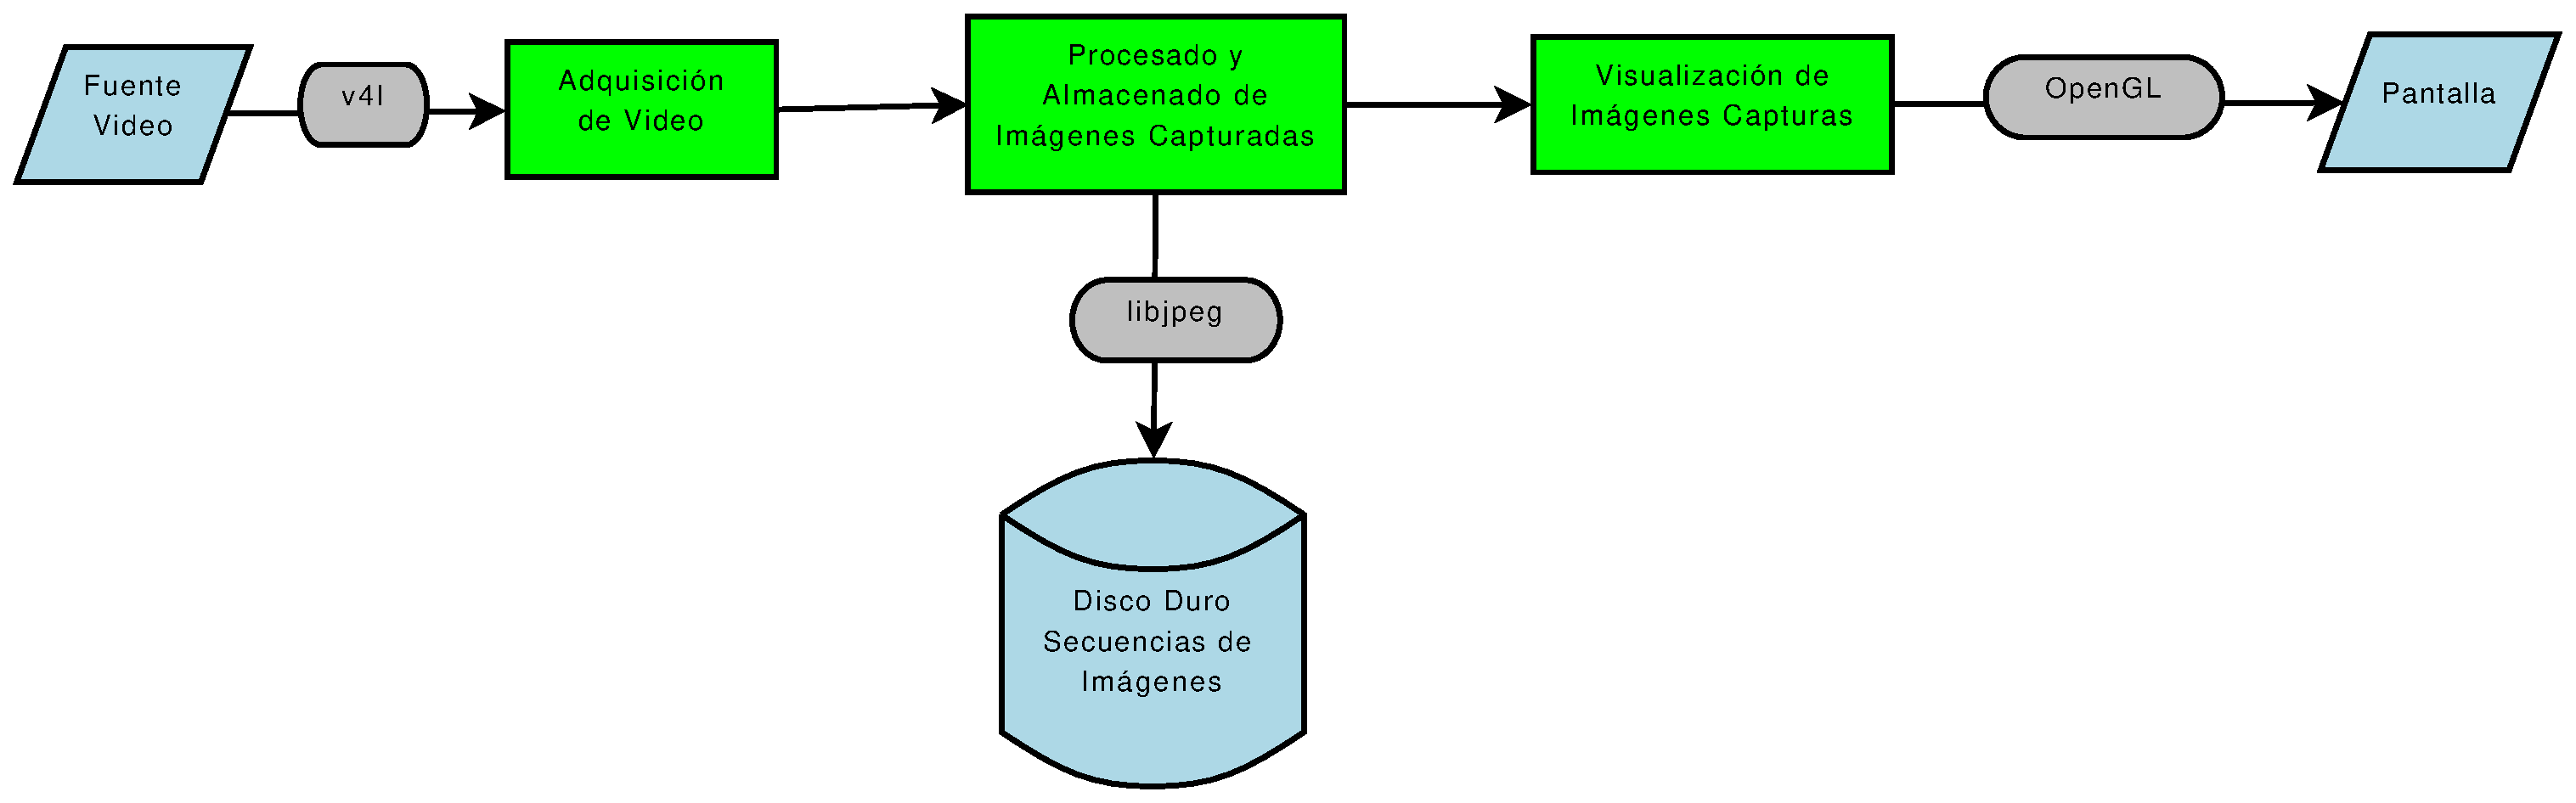
\includegraphics[width=13.0cm,angle=0]{images/murapido/arquitectura.eps}

{\footnotesize\bf Arquitectura de nuestro sistema. Hardware, Software y APIs}
\end{figure}

\clearpage
\pagebreak

\bOpage{introcolor}{0.25}{M� R�PIDO}

Si dispon�is de una tarjeta capturadora de TV BT848, necesitar�is una
fuente de v�deo adicional, una c�mara externa o, en su defecto, un DVD
o magnetoscopio. Si utiliz�is la salida de v�deo 
compuesto, el c�digo que vamos a comentar en el art�culo deber�a funcionar
casi sin modificaciones. Si, lo que quer�is es utilizar la entrada de
RF (la de la antena), ser�n necesarias algunas modificaciones. Os
daremos algunas indicaciones de como hacerlas pero, por cuestiones de
espacio, no las vamos a incluir aqu�.

\begin{entradilla}
{\em Un par de {\color{introcolor} webcams} nos servir�n para nuestro prototipo.}
\end{entradilla}

En nuestro caso concreto, el de las webcams Logitech Messenger,
tenemos que hacer un par de comentarios. El primero es que parece que
las c�maras (o m�s bien el driver) no funciona correctamente si se
conectan a trav�s de un HUB USB externo. Para poder utilizarlas deben
estar conectadas directamente a los puertos USB del ordenador.

El segundo problema que nos encontramos con estas c�maras, fue que el
driver no soporta m�s de un dispositivos del mismo tipo. Mardita sea!.

\sectiontext{white}{black}{ARREGLANDO EL DRIVER}

Aunque para lo que os vamos a contar en este art�culo, podr�amos
utilizar una �nica c�mara, a nosotros nos interesaba poder utilizar
dos o m�s para poder hacer cosas m�s g�ays.... os suenan esas gafas rojas y
azules?.

As� que nos bajamos el driver y le echamos un ojo, con la esperanza de
poder modificarlo f�cilmente para que nuestras dos c�maras
funcionaran. Bendito software libre!. 

Con la informaci�n de depuraci�n del driver y mucha suerte, encontramos que el ``problema''
estaba en la funci�n \verb!gspca_init_transfert!. 

Por cada dispositivo, esta funci�n ``reparte'' lo que en los logs
aparece como un ``AlternateSet''. Cuando la primera c�mara es
inicializada, la funci�n le asigna todos los ``recursos'' (por llamarlos
de alguna forma) y al intentar inicializar la segunda, se produce un
error, ya que, aparentemente no hay ``recursos'' que asignarle (los
tiene todos la primera c�mara). 

Los recursos no son otra cosa que el
ancho de banda USB que se asigna a ese dispositivo. En la FAQ de
motion, podr�is encontrar algunos detalles m�s sobre como utilizar
varias c�maras USB. B�sicamente necesitar�ais una segunda tarjeta
USB. Como nosotros no la tenemos, hemos optado por este parche, como
soluci�n de compromiso.

Para ello, a�adimos un nuevo par�metro al driver que
llamamos \verb!ndevices!. Las modificaciones en el fichero \verb!gspca_core.c!
fueron las siguientes:

\columnbreak

\lstset{language=C,frame=tb,framesep=5pt,basicstyle=\scriptsize}   
\begin{lstlisting}
static int ndevices = 1;

module_param(ndevices, int, 0644);
MODULE_PARM_DESC(ndevices, "Number of devices to"
                           " use simultaneously.");
\end{lstlisting}

Esta nueva variable la utilizamos en la
funci�n \verb!gspca_init_transfert! para modificar el valor de la
variable \verb!nbalt!, de la siguiente forma: 

\lstset{language=C,frame=tb,framesep=5pt,basicstyle=\scriptsize}   
\begin{lstlisting}
intf = usb_ifnum_to_if(dev, spca50x->iface);
nbalt = intf->num_altsetting - 1;

/* Nuestra nueva l�nea */
nbalt = nbalt / ndevices;
\end{lstlisting}

Por supuesto esto es un hack ``m� r�pido'' y probablemente haya mejores
formas de hacerlo, pero para las pruebas que nosotros vamos a hacer es
m�s que suficiente.

Ahora podemos cargar nuestra nueva versi�n del driver, de la siguiente
forma:

{\small
\begin{verbatim}
# rmmod gspca
# insmod ./gspca.ko ndevices=2
\end{verbatim}
}

Et voil�!.... tenemos nuestras dos webcams disponibles.

Para comprobar que todo funciona correctamente, pod�is utilizar la
aplicaci�n spcaview descargable desde la p�gina del driver gspca. Este
programa es especialmente interesante ya que se trata de un ejemplo
completo de como manejar un dispositivo soportado por este driver. 

Como esta es la secci�n "m� r�pido", nuestro interfaz V4L va a ser muy
simpl�n, y estudiar esta aplicaci�n os permitir� extenderlo si quer�is
hacer que vuestros programas funcionen en el caso general.

\begin{entradilla}
{\em Para la captura de im�genes utilizaremos el {\color{introcolor} API V4L}}
\end{entradilla}

Si vuestro hardware utiliza otro driver, probad con alguna aplicaci�n
est�ndar como {\em camorama} o {\em cheese}.

\sectiontext{white}{black}{CAPTURANDO VIDEO}

Despu�s de todos estos preparativos vamos al ajo :). Lo primero que
vamos a hacer es nuestro m�dulo de captura de v�deo. En esta versi�n
supersimplificada, nuestro m�dulo tendr� tres funciones. Aqu� ten�is los prototipos.

\lstset{language=C,frame=tb,framesep=5pt,basicstyle=\scriptsize}   
\begin{lstlisting}
int open_v4l (DISP d, char *d, int *w, int *h);
void start_v4l (DISP d);
char *capture_v4l_full (DISP d);
\end{lstlisting}

La primera de las funciones abre e inicializa el dispositivo de
captura. La segunda le dice al dispositivo que comience a capturar
video. Por �ltimo, la tercera, nos permite obtener la �ltima imagen
capturada por el dispositivo.

\ebOpage{introcolor}{0.25}{M� R�PIDO}

Para poder utilizar el API V4L, necesitamos los siguientes includes en
nuestro c�digo:



\lstset{language=C,frame=tb,framesep=5pt,basicstyle=\scriptsize}   
\begin{lstlisting}
#include <sys/ioctl.h>
#include <fcntl.h>

#include <sys/mman.h>
#include <linux/videodev.h>
\end{lstlisting}

El primero es necesario para utilizar la llamada al sistema \verb!ioctl!, con
la que poder enviar mensajes al driver. El segundo solo es
necesario para la llamada al sistema \verb!open!, con la que acceder al
dispositivo de captura. En seguida veremos como utilizarla.

El tercero lo necesitamos para el proceso de captura. Nosotros vamos a
utilizar un mapeado de memoria en lugar del m�todo \verb!read!. 

Finalmente, el �ltimo de los includes es el que define todas las
estructuras de datos espec�ficas de los dispositivos de video. La
mayor�a de las estructuras de datos que utiliza la funci�n \verb!open_v4l!
est�n definidas aqu�.

Para poder utilizar m�s de un dispositivo de captura de video, hemos
definido una estructura muy sencilla en la que almacenar los datos
espec�ficos de cada uno de ellos. Esta es:

\lstset{language=C,frame=tb,framesep=5pt,basicstyle=\scriptsize}   
\begin{lstlisting}
typedef struct disp_t {
  int                fd;
  struct video_mbuf  mbuf_info;
  struct video_mmap  mmap_info;
  /* Mapa de memorua de datos de video */
  char               *mm;
  char               *buffer;
  /* Informaci�n sobre la imagen */
  int                w, h, canal, bpp;
  double             brillo, contraste, color;
} *DISP;
\end{lstlisting}

El uso de cada uno de estos campos quedar� claro en cuanto describamos
las funciones de nuestro interfaz... esto es, ya mismo :)


\sectiontext{white}{black}{ABRIENDO EL DISPOSITIVO}

La funci�n \verb!open_v4l! es la que se encarga de la inicializaci�n del
dispositivo de captura de v�deo, y es la m�s larga de todas, por esa
raz�n la iremos comentando por partes, para que sea m�s f�cil seguirla.

Lo primero que nos encontramos es esto:

\lstset{language=C,frame=tb,framesep=5pt,basicstyle=\scriptsize}   
\begin{lstlisting}
  struct video_capability dev_info;
  struct video_channel    channel_info;
  struct video_picture    picture_info;

  /* Abrimos el dispositivo de video */
  if ((d->fd = open (device, O_RDWR)) < 0)
    {    
      fprintf (stderr, "No puedo abrir "
                       "dispositivo %s\n", 
                       device);
      return (-1);
    }
\end{lstlisting}

La funci�n comienza declarando tres variables locales que utilizaremos
durante la inicializaci�n del dispositivo, para, a continuaci�n, abrir
el dispositivo. 

Dos comentarios aqu�. El primero es que hemos eliminado todas las
comprobaciones de error con la excepci�n de esta primera. Si el
dispositivo se abre, muy probablemente todo vaya como la seda, pero si
esto falla, nada funcionar�.

El segundo es que los dispositivos de v�deo, tienen nombres como \verb!/dev/video1! o
\verb!/dev/video2!. Tendremos tantos como dispositivos de captura hayamos instalado
en el sistema. Si vuestro hardware de captura est� correctamente
instalado los dispositivos deber�an estar ah�.

\sectiontext{white}{black}{CONFIGURANDO CANALES}

El siguiente paso consiste en configurar el canal del dispositivo que
vamos a utilizar. Si est�is utilizando una webcam como nosotros,
probablemente solo teng�is un canal. Pero si est�is utilizando
una tarjeta de captura de televisi�n, normalmente tendr�is al menos 2
canales. Uno para la entrada de video compuesto (o banda base) y otro para el
sintonizador de televisi�n. 

\begin{entradilla}
{\em Video 4 Linux nos permite {\color{introcolor} configurar los par�metros} de captura de
nuestra webcam}
\end{entradilla}

Si os
veis obligados a utilizar la entrada del sintonizador de televisi�n,
tendr�is que configurar el canal correcto, y programar el sintonizador
para seleccionar el canal (de la TV) que quer�is capturar.

No vamos a explicar como hacer todo esto, pero si alguien est�
utilizando una tarjeta de captura TV, le recomendamos que utilice la
librer�a libbgrab.

Volviendo al c�digo...

\lstset{language=C,frame=tb,framesep=5pt,basicstyle=\scriptsize}   
\begin{lstlisting}
  /* Conseguimos las caracteristicas */
  ioctl (d->fd, VIDIOCGCAP, &dev_info);
 
  /* Nos quedamos con el ancho y alto m�ximos */
  d->w = dev_info.maxwidth;
  d->h = dev_info.maxheight;

  *w = d->w;
  *h = d->h;
  
  /*Usamos canal 0. Entrada de video compuesto*/
  channel_info.channel = d->canal;

  /*Obtenemos informaci�n del canal seleccionado*/
  ioctl (d->fd, VIDIOCGCHAN, &channel_info);

  /*Activamos modo PAL*/
  channel_info.norm = 0;

  /*Actualizamos la informaci�n del canal*/
  ioctl (d->fd, VIDIOCSCHAN, &channel_info);
\end{lstlisting}

Como adelantamos m�s arriba, la forma de ``hablar'' con el driver es a trav�s de
la llamada al sistema \verb!ioctl!. Para la configuraci�n del canal,
utilizamos tres mensajes. \verb!VIDIOCGCAP!, algo as� como "VIDeo Input Output
Chanel Get Capabilities"... vamos digo yo :), con lo que obtenemos las
caracter�sticas del dispositivo, la informaci�n sobre sus canales. En
nuestro ejemplo, estamos utilizando este 
mensaje para obtener el ancho y alto m�ximo de las im�genes que pueden
ser capturadas utilizando este canal y almacen�ndolas en nuestra
estructura para su uso posterior.

\ebOpage{introcolor}{0.25}{M� R�PIDO}

Estos valores los retornamos a la aplicaci�n principal, ya que los
necesitaremos para la visualizaci�n de las im�genes.

El siguiente mensaje es \verb!VIDIOCGCHAN!, con el que obtenemos informaci�n
sobre el canal de inter�s. El canal de inter�s se indica utilizando el
campo \verb!channel! de la estructura de datos \verb!video_channel! (variable
\verb!channel_info!). La informaci�n sobre el canal se retorna sobre esa
misma estructura de datos.

\begin{entradilla}
{\em Los dispositivos de {\color{introcolor} captura de im�genes}
pueden proporcionar varios {\color{introcolor}canales}}
\end{entradilla}

Finalmente, utilizamos el mensaje \verb!VIDIOCSCHAN! (la s es de SET), para
configurar el canal. Lo que estamos haciendo es coger la configuraci�n
del canal (\verb!VIDIOCGCHAN!), modificando solamente la norma de video a PAL y
reconfigurando el canal de nuevo (\verb!VIDICSCHAN!).

Puede que dependiendo de vuestro hardware teng�is que modificar alg�n
campo m�s para configurar apropiadamente el canal, o que no necesit�is
modificar la norma de v�deo para vuestro dispositivo. Ah� tendr�is que
investigar un poco por vuestra cuenta.

Hemos intentado reducir al m�nimo el c�digo de
inicializaci�n salt�ndonos varias comprobaciones que ser�an necesarias
en una aplicaci�n ``profesional''. Si algo falla, coged el c�digo de
alguno de los programas incluido en vuestra distribuci�n que funcione
correctamente, y empezad a a�adir las partes que faltan... eso es lo que nosotros hemos hecho :).

\sectiontext{white}{black}{PAR�METROS DE IMAGEN}

Ahora que hemos seleccionado y configurado nuestro canal, tenemos que
proporcionar al driver una serie de par�metros, para decirle como
queremos las im�genes.

Aqu� pod�is ver como hacerlo.

\lstset{language=C,frame=tb,framesep=5pt,basicstyle=\scriptsize}   
\begin{lstlisting}
/* Ahora los par�metros de imagen */
picture_info.brightness = (int)(65535*d->brillo);
picture_info.hue        = 0;
picture_info.colour     = (int)(65535*d->color);
picture_info.contrast   = (int)(65535*d->contraste);
picture_info.whiteness  = 0;
picture_info.depth      = 24;
picture_info.palette    = VIDEO_PALETTE_RGB24;

ioctl (d->fd, VIDIOCSPICT, &picture_info);
\end{lstlisting}

La estructura \verb!video_picture! (variable \verb!picture_info!), nos permite
configurar el brillo, contraste y color de la imagen, entre otros
par�metros. Dependiendo si la captura es en color o escala de grises
ciertos par�metros no tienen efecto. 

Todos estos valores se codifican como un entero entre 0 y 65535, y
nosotros los proporcionamos como valores reales entre 0 y 1
representando un porcentaje. 

Pero los datos importantes son los dos �ltimos (\verb!depth! y
\verb!palette!). Estos campos nos permiten configurar la profundidad de color
y el formato de la imagen que vamos a obtener. Nosotros estamos
utilizando 24 bits por pixel (True Color) y un formato RGB de 24 bits,
ya que esto va ha hacer nuestro c�digo de visualizaci�n mucho m�s
sencillo.

Estos par�metros dependen del hardware de captura e idealmente, el
programa, debe utilizar las \verb!ioctl! apropiadas para preguntar al driver
que formatos soporta y configurarlo apropiadamente. La
configuraci�n que estamos utilizando es bastante est�ndar y deber�a
funcionar en la mayor�a de los casos, pero quiz�s teng�is que
modificar estos valores para que funcionen en vuestro hardware.

Obviamente el mensaje \verb!VIDIOCSPICT! es el que nos permite pasar estos
datos al driver (ya sab�is Set PICTure).

\sectiontext{white}{black}{CONFIGURANDO LA TRANSFERENCIA DE DATOS}

El �ltimo paso que nos falta para completar el proceso de
inicializaci�n es la configuraci�n de transferencia de datos. Como
adelant�bamos un poco m�s arriba, hay dos formas de transferir las
im�genes a nuestro programa. Una es utilizando la llamada al sistema
\verb!read! y otra es utilizando mapeado de memoria con la llamada al sistema
\verb!mmap!.

Nosotros utilizamos el mapeado de memoria, porque mola m�s y adem�s
podemos utilizar doble buffer para la captura. El c�digo es el
siguiente:

\lstset{language=C,frame=tb,framesep=5pt,basicstyle=\scriptsize}   
\begin{lstlisting}
  /* Obtenemos mapa  de meoria */
  ioctl (d->fd, VIDIOCGMBUF, &d->mbuf_info);

  /* Vamos a trabajar con doble buffer */
  if (d->mbuf_info.frames < 2)
    exit (1);
\end{lstlisting}

Lo primero que hacemos es preguntarle al driver los detalles para el
mapeado de memoria, utilizando , una vez m�s, la llamada al sistema
\verb!ioctl!. En la estructura \verb!video_mbuf! (uno de los campos de nuestra
estructura \verb!DISP!), obtendremos el resultado.

\begin{entradilla}
{\em Nuestra aplicaci�n captura las im�genes utilizando
{\color{introcolor} mapeado de memoria}}
\end{entradilla}

�Y cuales son los detalles para el mapeado de memoria? Os
preguntar�is. B�sicamente son los siguiente: El n�mero de cuadros que
el dispositivo es capaz de capturar, el tama�o de la zona de memoria
en la que el driver va a poder los datos de la imagen y los
desplazamientos, dentro de ese bloque de memoria, donde se almacenar�n
los distintos cuadros. 

Todo esto tomar� sentido muy pronto, en cuanto os mostremos una
sencilla figura :).

\end{multicols}

\clearpage
\pagebreak

\msection{introcolor}{black}{0.25}{M� R�PIDO}

\begin{figure}[ht]
\centering
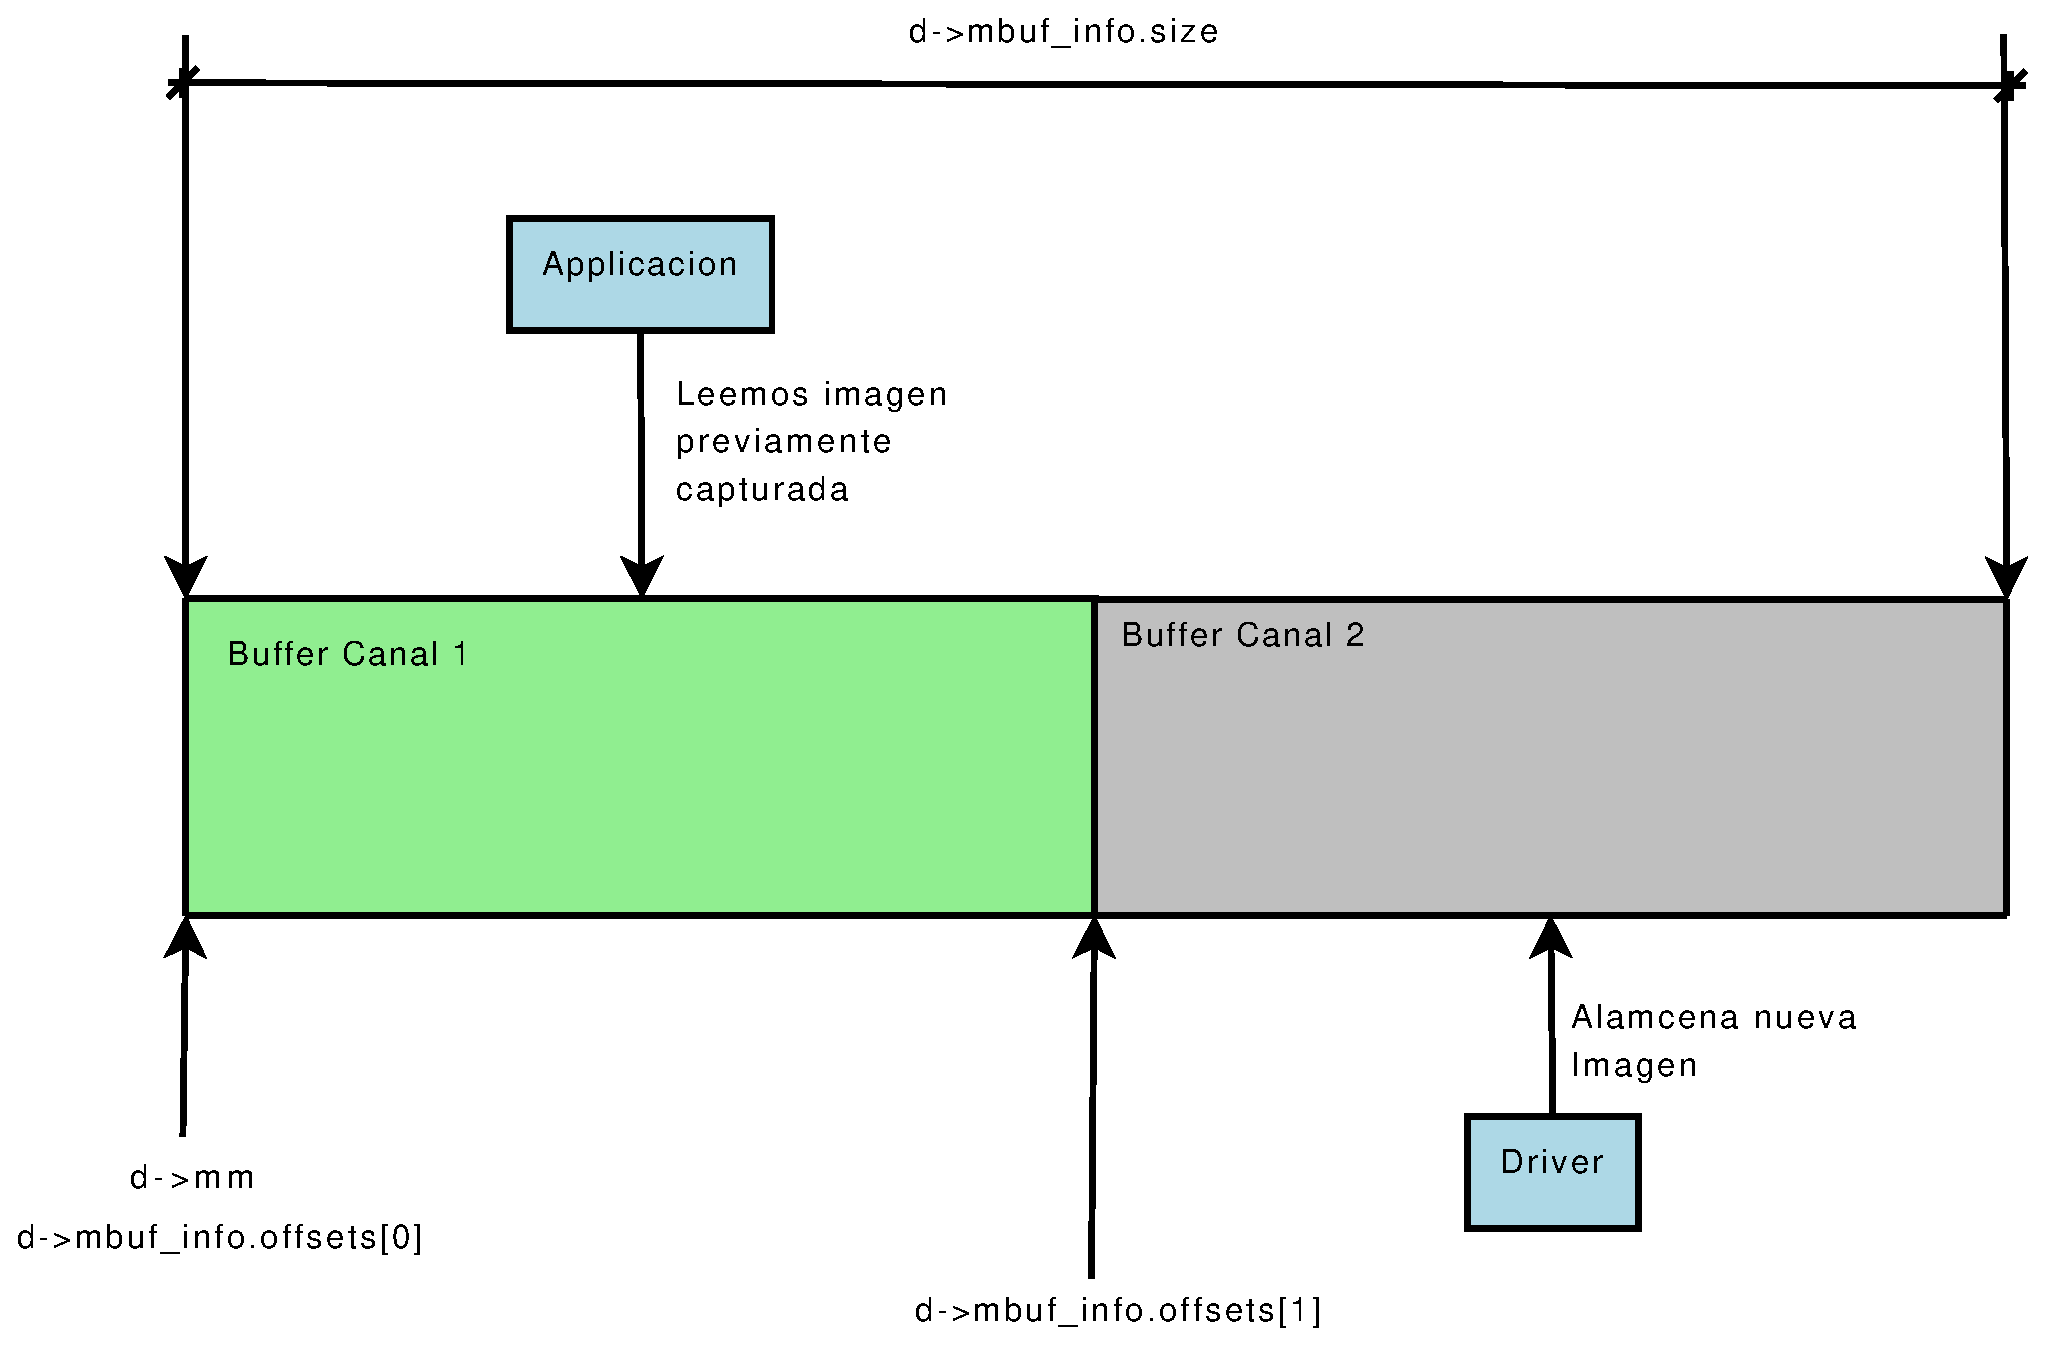
\includegraphics[height=8.0cm,angle=0]{images/murapido/v4l_doble_buffer.eps}
\end{figure}

\bigskip

\begin{multicols}{2}

En nuestro ejemplo, utilizamos doble buffer. Esta
t�cnica consiste en utilizar dos bloques de memoria para adquirir los
datos, de tal forma que cuando el driver est� capturando un cuadro, lo
est� almacenando en uno de esos buffers y as�, nosotros podemos acceder
al otro (el cuadro anterior) sin que nadie nos moleste.

\begin{entradilla}
{\em Utilizando {\color{introcolor} doble buffer} podemos capturar una imagen, mientras
procesamos otra}
\end{entradilla}

Cuando el cuadro actual haya sido capturado, los buffers se
intercambian y nuestra aplicaci�n puede acceder al nuevo cuadro a la
vez que el driver captura los datos del siguiente cuadro y los
almacena en el otro buffer. 

Por esa raz�n terminamos nuestra aplicaci�n si el driver no es capaz
de proporcionarnos al menos dos buffers. Si por alguna raz�n vuestro
hardware/driver no soporta m�s que un buffer, pod�is eliminar esa
comprobaci�n, pero tendr�is que hacer unos peque�os cambios al resto
de las funciones de este m�dulo. 

Una vez obtenida esta informaci�n, utilizamos la llamada al sistema
\verb!mmap! para mapear la memoria, es decir, para permitir a nuestra
aplicaci�n acceder a los buffers que el driver est� utilizando y, por
tanto, acceder a los datos de las im�genes capturadas.

\lstset{language=C,frame=tb,framesep=5pt,basicstyle=\scriptsize}   
\begin{lstlisting}
  /* Mapeamos memoria para acceder a las imagenes*/
  d->mm = (char *)mmap (0, d->mbuf_info.size, 
			PROT_READ | PROT_WRITE, 
                        MAP_SHARED, 
			d->fd, 0);
\end{lstlisting}

Finalmente, reservamos un buffer adicional en el que almacenaremos una
copia de la imagen capturada, e inicializamos el campo \verb!mmap_info! con
los datos que necesitaremos durante la captura real de las im�genes.

\lstset{language=C,frame=tb,framesep=5pt,basicstyle=\scriptsize}   
\begin{lstlisting}
  d->buffer = malloc (d->mbuf_info.size);
  
  /* Estructura para el mapeo de memoria */
  d->mmap_info.frame  = 0;
  d->mmap_info.width  = d->w;
  d->mmap_info.height = d->h;
  d->mmap_info.format = picture_info.palette;
\end{lstlisting}

En este punto, nuestro hardware de captura est� listo para empezar a
``escupir'' im�genes... pero, �c�mo las obtenemos?... enseguida lo
veremos.

\sectiontext{white}{black}{INICIANDO LA CAPTURA}

El proceso de captura lo hemos dividido en dos funciones, una que
inicia el proceso y otra que obtiene los datos de la imagen.

La primera pinta tal que as�:

\lstset{language=C,frame=tb,framesep=5pt,basicstyle=\scriptsize}   
\begin{lstlisting}
void start_v4l (DISP d)
{
  d->mmap_info.frame = 0;
  ioctl (d->fd, VIDIOCMCAPTURE, &d->mmap_info);
  d->mmap_info.frame = 1;
  ioctl (d->fd, VIDIOCMCAPTURE, &d->mmap_info);
  d->mmap_info.frame = 0;
}
\end{lstlisting}

Esta funci�n utiliza el mensaje \verb!VIDIOCMCAPTURE! y espera como par�metro
una estructura del tipo \verb!video_mmap!. El campo \verb!frame!, le dice al driver
que cuadro capturar, o dicho de otra forma, que parte del buffer
utilizar.

Con lo que acabamos de comentar, deber�a estar claro lo que hace la
funci�n. Inicia la captura de los dos frames y nos devuelve el
control mientras el hardware hace su trabajo.

A partir de ese momento, nuestra aplicaci�n principal entrar� en un
bucle infinito, en que llamar� continuamente a la funci�n \verb!capture_v4l!
que os mostramos a continuaci�n: 

%%%%%%%%%%%%%%%%%%%%%%%%%%%%%%%%%%%%%%%%%%%%%%%%%%%%%%%%%%%%%%%%%%%
\ebOpage{introcolor}{0.25}{M� R�PIDO}

\lstset{language=C,frame=tb,framesep=5pt,basicstyle=\scriptsize}   
\begin{lstlisting}
char *capture_v4l (DISP d)
{
  ioctl (d->fd, VIDIOCSYNC, &d->mmap_info.frame);

  memcpy (d->buffer, d->mm + 
          d->mbuf_info.offsets[d->mmap_info.frame], 
	  d->mbuf_info.size / 2);

  ioctl (d->fd, VIDIOCMCAPTURE, &d->mmap_info);
  d->mmap_info.frame = 1 - d->mmap_info.frame;

  return d->buffer;
}
\end{lstlisting}

Lo primero que hace la funci�n es enviar el mensaje \verb!VIDIOCSYNC!. Este
mensaje hace que nuestro programa espere hasta que el cuadro
que se pasa como par�metro est� listo. Que significa que est�
listo?. Pues que la parte del buffer asociada a ese cuadro, contenga
una imagen completa.

\begin{entradilla}
{\em Nuestro {\color{introcolor} sencillo interfaz con V4L}, nos permite capturar im�genes
de forma sencilla}
\end{entradilla}

Una vez que tenemos una imagen disponible (cuando \verb!ioctl! retorna),
copiamos inmediatamente la imagen a nuestro buffer temporal. En
principio, esto no ser�a necesario, pero en las distintas pruebas que
hemos hecho, cuando utilizamos m�s de un dispositivo los buffers se
corrompen, si bien, esto puede ser debido a que el programa es muy
tonto, o simplemente que nuestro USB no da para m�s :(. Aqu� ten�is
algo interesante para investigar ;).

Si solo est�is utilizando un dispositivo, pod�is utilizar directamente
el puntero de la zona de memoria mapeada. Esto ser�a:

\lstset{language=C,frame=tb,framesep=5pt,basicstyle=\scriptsize}   
\begin{lstlisting}
d->mm + d->mbuf_info.offsets [d->mmap_info.frame]
\end{lstlisting}

Con lo que os ahorr�is la copia de los datos, pero es necesaria una
peque�a modificaci�n del resto del c�digo.

Finalmente, se inicia de nuevo la captura del frame que acabamos de
copiar con el mensaje \verb!VIDIOCMCAPTURE! y se actualiza el campo, para que
en la pr�xima llamada a la funci�n trabajemos sobre el otro buffer,
que deber�a contener ya la siguiente imagen.

\sectiontext{white}{black}{EL PROGRAMA PRINCIPAL}

Ahora que ya tenemos nuestro interfaz de captura de im�genes, estamos
en condiciones de escribir nuestra aplicaci�n de captura de im�genes :).

El programa principal, adem�s de utilizar nuestro flamante interface
para V4L, mostrar� en una ventana las im�genes capturadas. Para ello
vamos a utilizar OpenGL, pero para el interfaz entre OpenGL y el
sistema de ventanas vamos a utilizar GLUT (GL Utility Toolkit), que va
a hacer nuestra vida mucho m�s f�cil.... GLX y Xlib son un poco m�s
engorrosos. 

Aqu� ten�is el programa principal.

\lstset{language=C,frame=tb,framesep=5pt,basicstyle=\scriptsize}   
\begin{lstlisting}
DISP d[2];

int main (int argc, char *argv[])
{
  /* Creamos dispositivos */
  d[0] = create_dev();
  d[1] = create_dev();

  /* Inicializa GLUT */
  glutInit (&argc, argv);
  glutInitDisplayMode (GLUT_RGBA | GLUT_DOUBLE 
                                 | GLUT_DEPTH);
  glutInitWindowSize (WIN_WIDTH, WIN_HEIGHT);
  glutCreateWindow ("Sistema Video Vigilancia "
                    "- Occam's Razor");
 
  /* Inicializa OpenGL */
  gfx_init ();
  
  /* Inicializa dispositivos de captura. 
     Terminamos ante cualquier error */
  open_v4l (d[0], "/dev/video1", &img_w, &img_h);
  start_v4l (d[0]);

  open_v4l (d[1], "/dev/video2", &img_w, &img_h);
  start_v4l (d[1]);
  
  /* Creamos las Texturas */
  init_texture (img_w, img_h);
  img_size = img_w * img_h * img_bpp;

  /* Configure GLUT callback handlers for events */
  glutDisplayFunc (gfx_pinta);
  glutKeyboardFunc (handle_keyboard);
  glutIdleFunc (handle_idle);
  
  /*Now we enter the main loop and process GLUT events*/
  glutMainLoop ();
  exit (0);
}
\end{lstlisting}

Si obviamos por un momento las llamadas a GLUT, el programa es muy
sencillo. Hemos utilizado una funci�n adicional (\verb!create_dev!) que
simplemente crea din�micamente un objeto del tipo \verb!DISP! (vamos, hace un
\verb!malloc!), y a continuaci�n llamamos a las funciones para inicializar
los dispositivos y comenzar la captura.


Lo que no vemos por ning�n lado es la llamada a \verb!capture_v4l!. Vale,
para encontrar esa llamada tenemos que explicaros un poco como
funciona GLUT.

\sectiontext{white}{black}{LA APLICACI�N GLUT}

Como ya habr�is intuido, todas las funciones de GLUT, empiezan
precisamente por glut :). Las primeras cuatro llamadas que nos
encontramos son las encargadas de crear la ventana en la que
mostraremos nuestro video.

\begin{entradilla}
{\em GLUT nos va a permitir utilizar OpenGL {\color{introcolor}m� r�pido}}
\end{entradilla}


Una explicaci�n detallada de GLUT se sale un poco de nuestro objetivo,
as� que no vamos a dar muchos detalles. Simplemente, las dos primeras
llamadas inicializan la librer�a, y normalmente van a ser siempre
as�. Las dos siguientes, como os pod�is imaginar, permiten definir el
tama�o de la ventana, y crearla especificando un t�tulo.

%%%%%%%%%%%%%%%%%%%%%%%%%%%%%%%%%%%%%%%%%%%%%%%%%%%%%%%%%%%%%%%%%%%
\ebOpage{introcolor}{0.25}{M� R�PIDO}

El siguiente bloque de llamadas a GLUT lo encontramos hacia el final,
y lo reproducimos de nuevo aqu� por comodidad:

\lstset{language=C,frame=tb,framesep=5pt,basicstyle=\scriptsize}   
\begin{lstlisting}
  glutDisplayFunc (gfx_pinta);
  glutKeyboardFunc (handle_keyboard);
  glutIdleFunc (handle_idle);
\end{lstlisting}

Estas tres funciones nos permiten definir ``call-backs''. Concretamente,
nos permiten decirle a GLUT que funci�n tiene que ejecutar cuando
tenga que actualizar la ventana, cuando se pulse una tecla y cuando no
tenga nada que hacer... s�, en esta �ltima es en la que vamos a capturar
nuestras im�genes.

Finalmente, la funci�n \verb!glutMainLoop! ejecuta un bucle infinito en el
que va llamando, seg�n convenga a cada una de los ``call-backs'' que
hemos definido.

\sectiontext{white}{black}{MANEJANDO EL TECLADO}

Vamos a empezar por esta funci�n, ya que es la m�s sencilla. El c�digo
es este:

\lstset{language=C,frame=tb,framesep=5pt,basicstyle=\scriptsize}   
\begin{lstlisting}
void 
handle_keyboard (unsigned char key, int x, int y)
{
  /* Process the input */
  switch (key)
    {
    case 'Q':
    case 27:
      exit (0);
      break;
      /* Control de la rotaci�n */
    case 'W':
      xangle += 5;
      break;
    case 'S':
      xangle -= 5;
      break;
    case 'A':
      zangle += 5;
      break;
    case 'D':
      zangle -= 5;
      break;      
    default:
      break;
    }
  
  /* Now refresh the display */
  gfx_pinta ();
}
\end{lstlisting}

Cada vez que el usuario pulsa una tecla, esta funci�n se ejecuta,
recibiendo como par�metro la tecla pulsada. Nuestro manejador, utiliza
la tecla Q o ESC (ASCII 27) para terminar la aplicaci�n. Las teclas A,
S, D y W se utilizan para actualizar las variables globales xangle e
yangle, que utilizaremos para rotar nuestros v�deos en 3D.

\sectiontext{white}{black}{CAPTURANDO}

La captura se realiza en la funci�n \verb!handle_idle!. Esta funci�n se
ejecuta en cada ciclo del bucle principal cuando no hay otra cosa que
hacer, es decir, no hay que actualizar el contenido de la ventana, no
se ha pulsado ninguna tecla ni se a movido el rat�n.

Esta funci�n ser�a algo tal que as�:

\columnbreak

\lstset{language=C,frame=tb,framesep=5pt,basicstyle=\scriptsize}   
\begin{lstlisting}
void handle_idle (void)
{
  char fname[1024];
  char *im, *im1;
  int  w, h, size, i, temp;

  im = capture_v4l_full (d[0]);
  im1 = capture_v4l_full (d[1]);

  /* Reordena componentes de color */
  for (i = 0; i < img_size; i+= img_bpp)
    {
      temp = *(im + i + 2);
      *(im + i + 2) = *(im + i + 0);
      *(im + i + 0) = temp;
    }

  for (i = 0; i < img_size; i+= img_bpp)
    {
      temp = *(im1 + i + 2);
      *(im1 + i + 2) = *(im1 + i + 0);
      *(im1 + i + 0) = temp;
    }

  /* Actualizamos nuestras texturas */
  change_texture (0, im);
  change_texture (1, im1);

  snprintf (fname, 1024, "video0-%05d.jpg", cnt);
  write_jpeg_file (fname, img);

  /* Redibujamos las nuevas imagenes */
  gfx_pinta ();
}
\end{lstlisting}

Lo primero que hacemos es obtener las �ltimas im�genes capturadas por
nuestros dispositivos. A continuaci�n tenemos que hacer un peque�o
procesado. En nuestro caso, las componentes azul y roja (2 y 0) de
cada pixel de la imagen est�n intercambiadas. Por alguna raz�n nuestra
c�mara nos devuelve la imagen en formato BGR en lugar de RGB.

Aunque podr�amos dejar que OpenGL se encargara de esto, hemos
preferido hacerlo a mano a modo de un sencillo procesado de
imagen. Pensad que en un sistema de v�deo vigilancia real, una de las
funcionalidades que se suelen requerir es la detecci�n de movimiento,
de forma que el sistema solo graba la secuencia de video cuando est�
pasando algo. Un mont�n de gigas de v�deo de una imagen est�tica no
valen para nada :).

\begin{entradilla}
{\em La captura de im�genes se realiza en el {\color{introcolor} callback IDLE} de GLUT}
\end{entradilla}

Ese tipo de procesado, o cualquier otra cosa que queramos hacer con
las im�genes, implica manipular sus pixels... y eso es lo que
hacen esos dos bucles tras las funciones de captura. 

Una vez que tenemos nuestras im�genes en el formato que queremos,
utilizamos la funci�n \verb!change_texture!, con la que modificaremos las
texturas OpenGL que utilizamos para visualizar el video. Muy pronto
veremos que hace esta funci�n exactamente.

Finalmente, llamamos a una funci�n \verb!write_jpeg_file! que grabar� las im�genes
en el disco en formato JPEG.

La funci�n termina ejecutando \verb!gfx_pinta! que es la encargada
de mostrar las im�genes en la ventana. Esta es nuestra siguiente v�ctima!

%%%%%%%%%%%%%%%%%%%%%%%%%%%%%%%%%%%%%%%%%%%%%%%%%%%%%%%%%%%%%%%%%%%
\ebOpage{introcolor}{0.25}{M� R�PIDO}

\sectiontext{white}{black}{VISUALIZANDO LA ESCENA}

La funci�n \verb!gfx_pinta! utiliza OpenGL para mostrar el v�deo en tiempo
real en un espacio 3D (echadle un ojo a la figura). Si sab�is algo de
OpenGL, ver�is que la funci�n es muy sencilla, sino, os comentaremos
solamente un par de cosas para que pod�is hacer algunos cambios.

\lstset{language=C,frame=tb,framesep=5pt,basicstyle=\scriptsize}   
\begin{lstlisting}
void gfx_pinta (void)
{
  glClear (GL_COLOR_BUFFER_BIT | 
           GL_DEPTH_BUFFER_BIT);
  
  /* Ponemos la prespectiva */
  glMatrixMode (GL_PROJECTION);
  glLoadIdentity ();
  gluPerspective (45.0, 
                 (double)WIN_WIDTH /
                 (double)WIN_HEIGHT, 
                 0.2, 20); 
  
  /* Pasamos a la matriz View Model */
  glMatrixMode (GL_MODELVIEW);  
  glLoadIdentity();
  
  /* Posicionamos la c�mara */
  gluLookAt (0, 4, 0,  /* Posici�n del Ojo */
	     0, 1, 0,  /* Punto al que miramos*/
	     0, 0, 1); /* Arriba */
  
  /* Rotamos la camara para efecto guay */
  glRotatef (zangle, 0, 0, 1);
  glRotatef (xangle, 1, 0, 0);

  glPushMatrix ();
  glTranslatef (-2.1, 0.0, 0.0);
  glScalef (scale, scale * ASPECT, scale);
  square_texture (0);

  glPopMatrix ();
  glTranslatef (0.1, 0.0, 0.0);
  glScalef (scale, scale * ASPECT, scale);
  square_texture (1);
   
  glutSwapBuffers ();
}
\end{lstlisting}

Lo primero que hace la funci�n es limpiar la pantalla (bueno, y el
z-buffer, pero eso ahora no nos interesa). A continuaci�n define la
matriz de proyecci�n o, en lenguaje llano, la perspectiva de la escena, esto es, el
campo de visi�n (que son 45 grados en nuestro ejemplo), el aspecto de
la ventana, el resto de par�metros no nos interesan en este ejemplo.

A continuaci�n se cambia a la matriz de modelo, que es la que tenemos
que utilizar para pintar cosas en 3D, y la inicializamos
(\verb!glLoadIdentity!), para luego posicionar la c�mara con \verb!gluLookAt!. Los
comentarios en el c�digo son suficientemente claros no?.

En este punto est� todo listo para que nuestros v�deos aparezcan en
pantalla. Como queremos ese interfaz 3D s�per g�ay de la muerte, lo
primero que hacemos es rotar la escena tanto en el eje Z como en el
X. Estos valores los podemos controlar con el teclado como ya hemos
visto. 

Esta transformaci�n (la rotaci�n definida con el teclado) la
vamos a aplicar a los dos v�deos que mostraremos en pantalla, as� que,
una vez calculada, nos la guardamos para usarla con la segunda
imagen. Esto es lo que hace la funci�n \verb!glPushMatrix!, almacena en una
pila la transformaci�n actual.

Movemos el primer v�deo un poco hacia la izquierda y los escalamos
seg�n el valor de la variable \verb!scale!. Pod�is ampliar la funci�n de
control de teclado para modificar este valor y hacer vuestros v�deos
m�s grandes o peque�os en pantalla. Como pod�is ver, la componente Y
se escala de forma diferente para mantener el aspecto de la imagen,
esto es, la relaci�n entre el ancho y el alto, en funci�n de las
dimensiones de nuestra ventana. Esto es necesario debido a la forma en
la que dibujamos los cuadros de nuestro v�deo. Lo veremos un poco
m�s adelante.

Finalmente dibujamos la imagen utilizando la funci�n
\verb!square_texture!. Observad que antes de dibujar la segunda imagen, hemos
recuperado nuestra transformaci�n inicial (\verb!glPopMatrix!), para, a
continuaci�n, posicionar la segunda imagen un poco a la izquierda.

Nosotros hemos colocado una imagen junto a la otra. Aunque visualmente
no parece tan g�ay, es m�s pr�ctico. Si quer�is el estilo ``Aero'',
tendr�is que modificar la componente Z de las traslaciones y hacer que
las im�genes se solapen modificando la componente X. 

La funci�n termina con una llamada a \verb!glutSwapBuffers! que env�a los
datos a la tarjeta. S�, OpenGL tambi�n utiliza doble buffer para la
visualizaci�n. Realmente pod�is activarlo o desactivarlo al
inicializar la librer�a (hab�is averiguado cual es el flag que hay que
eliminar?).

\end{multicols}

\begin{figure}[ht]
\centering
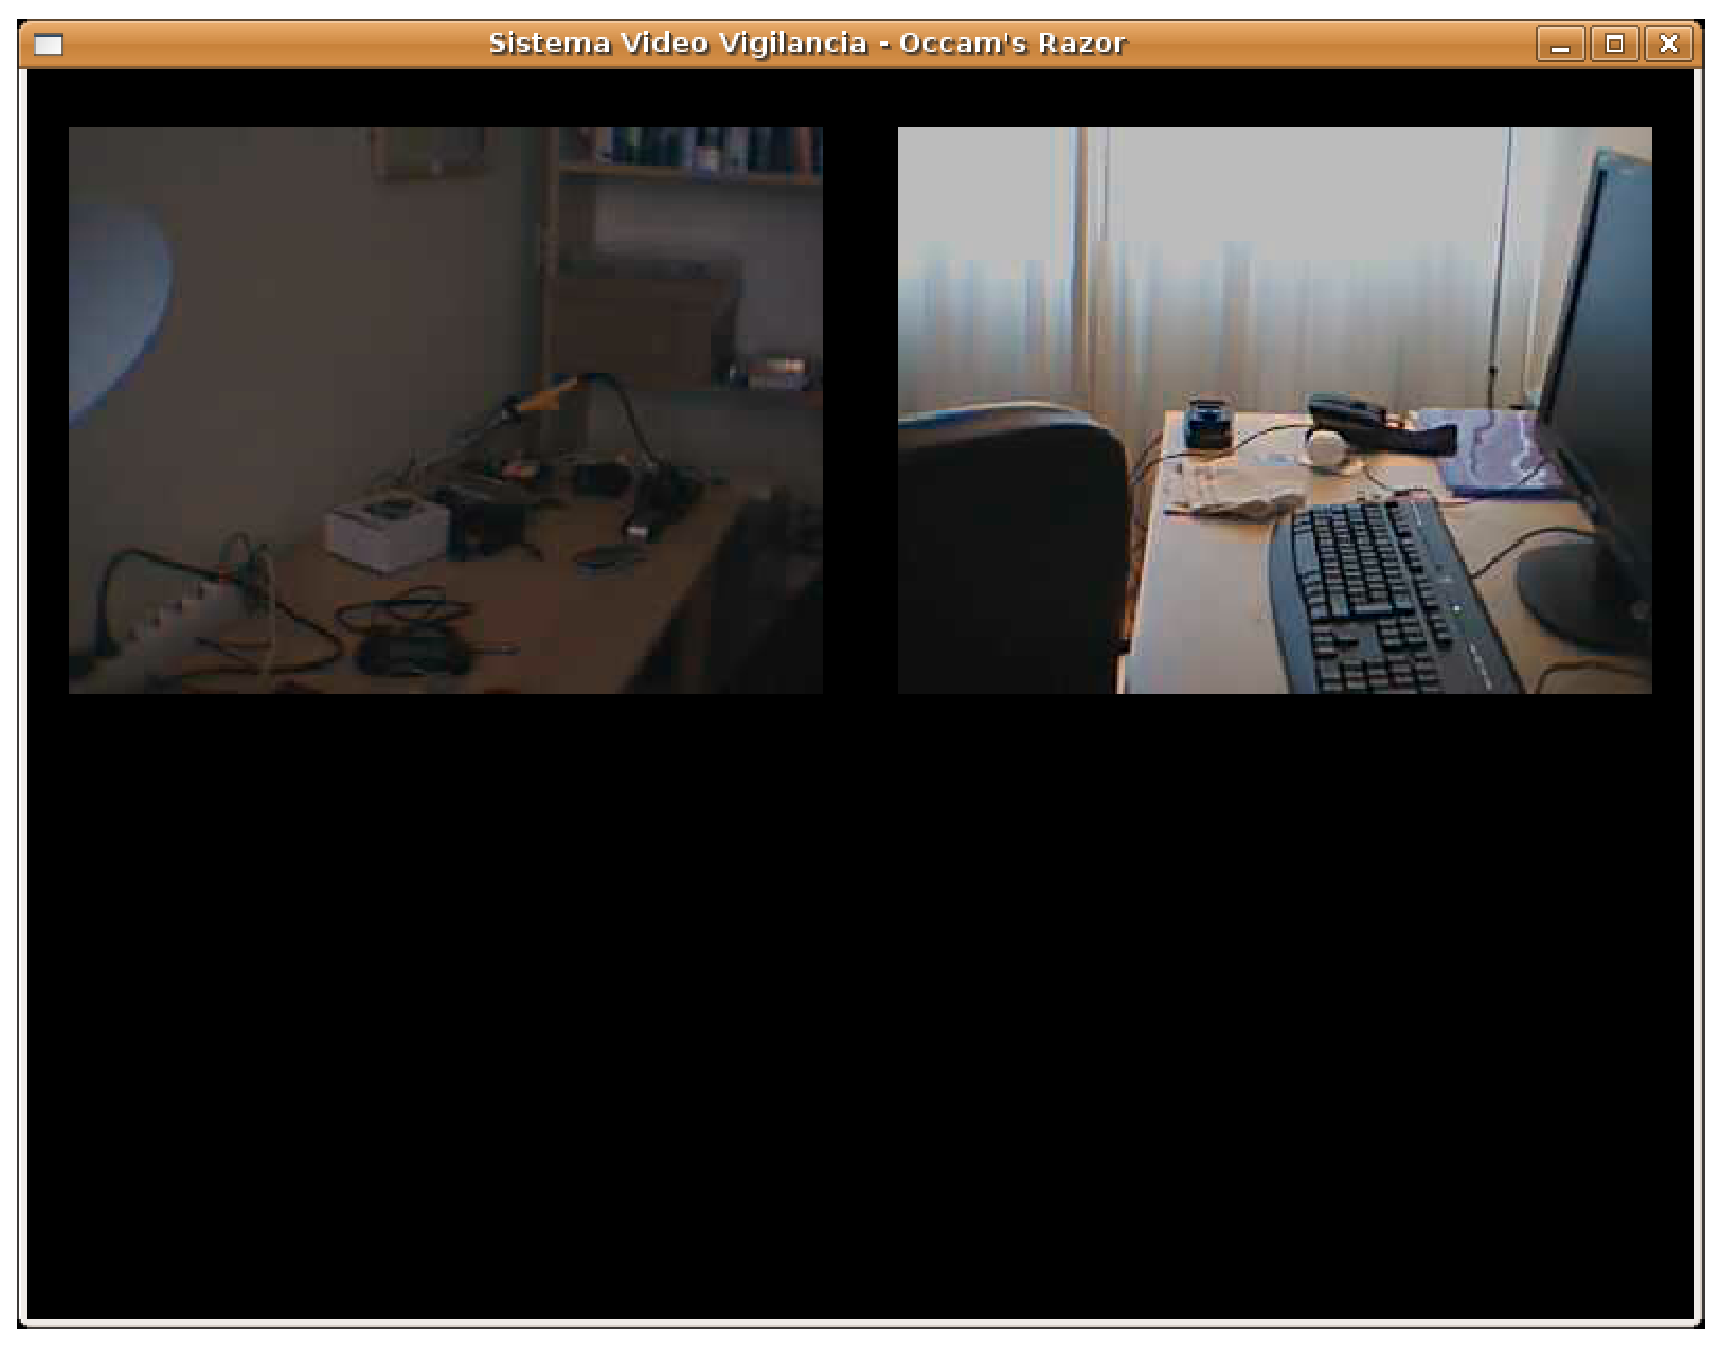
\includegraphics[height=5.5cm,angle=0]{images/murapido/shot00.eps}
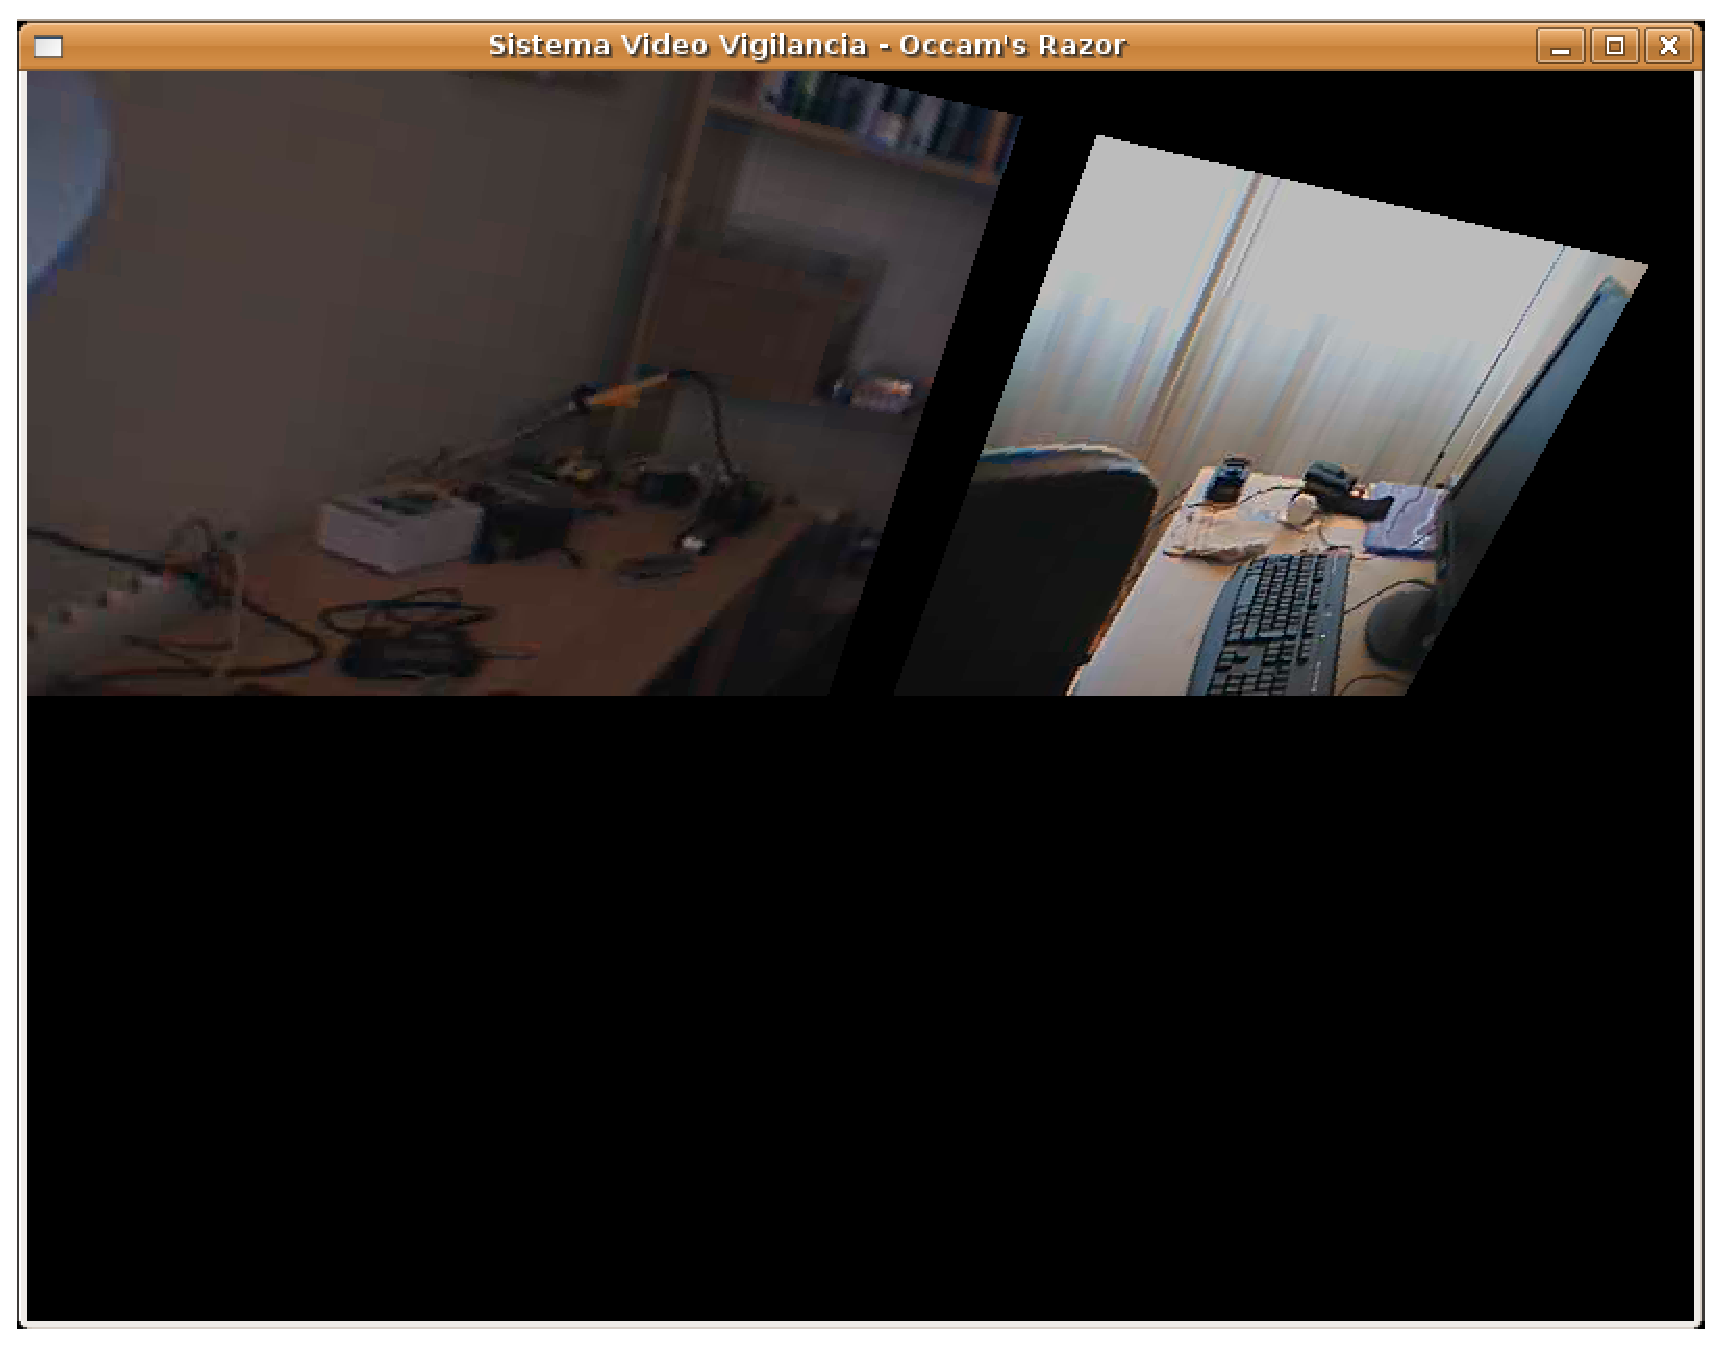
\includegraphics[height=5.5cm,angle=0]{images/murapido/shot01.eps}

{\footnotesize\bf Nuestra aplicaci�n. Izquierda: GUI normal. Derecha
GUI 3D}
\end{figure}


\clearpage
\pagebreak

%%%%%%%%%%%%%%%%%%%%%%%%%%%%%%%%%%%%%%%%%%%%%%%%%%%%%%%%%%%%%%%%%%%

\msection{introcolor}{black}{0.25}{M� R�PIDO}

\begin{figure}[ht]
\centering

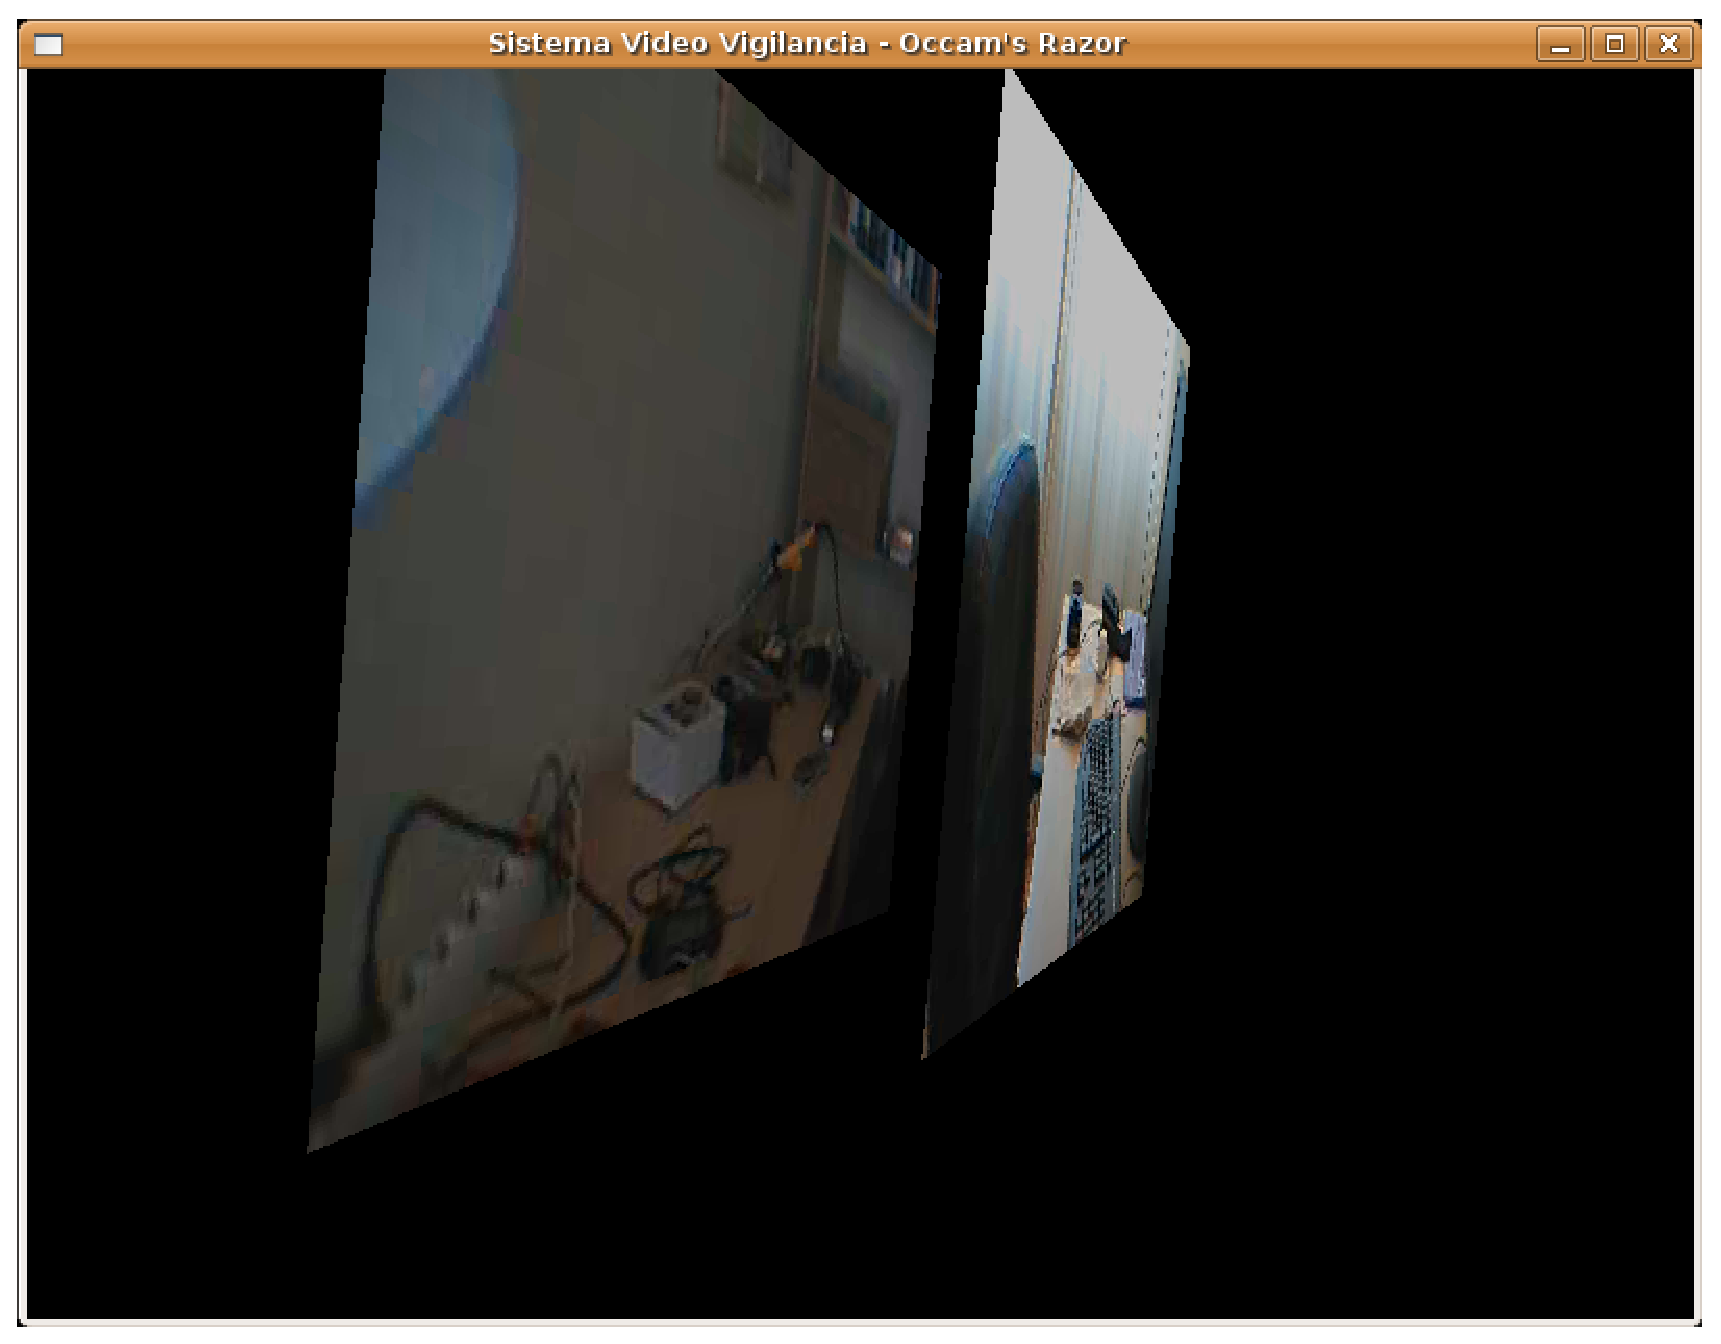
\includegraphics[height=5.5cm,angle=0]{images/murapido/shot05.eps}
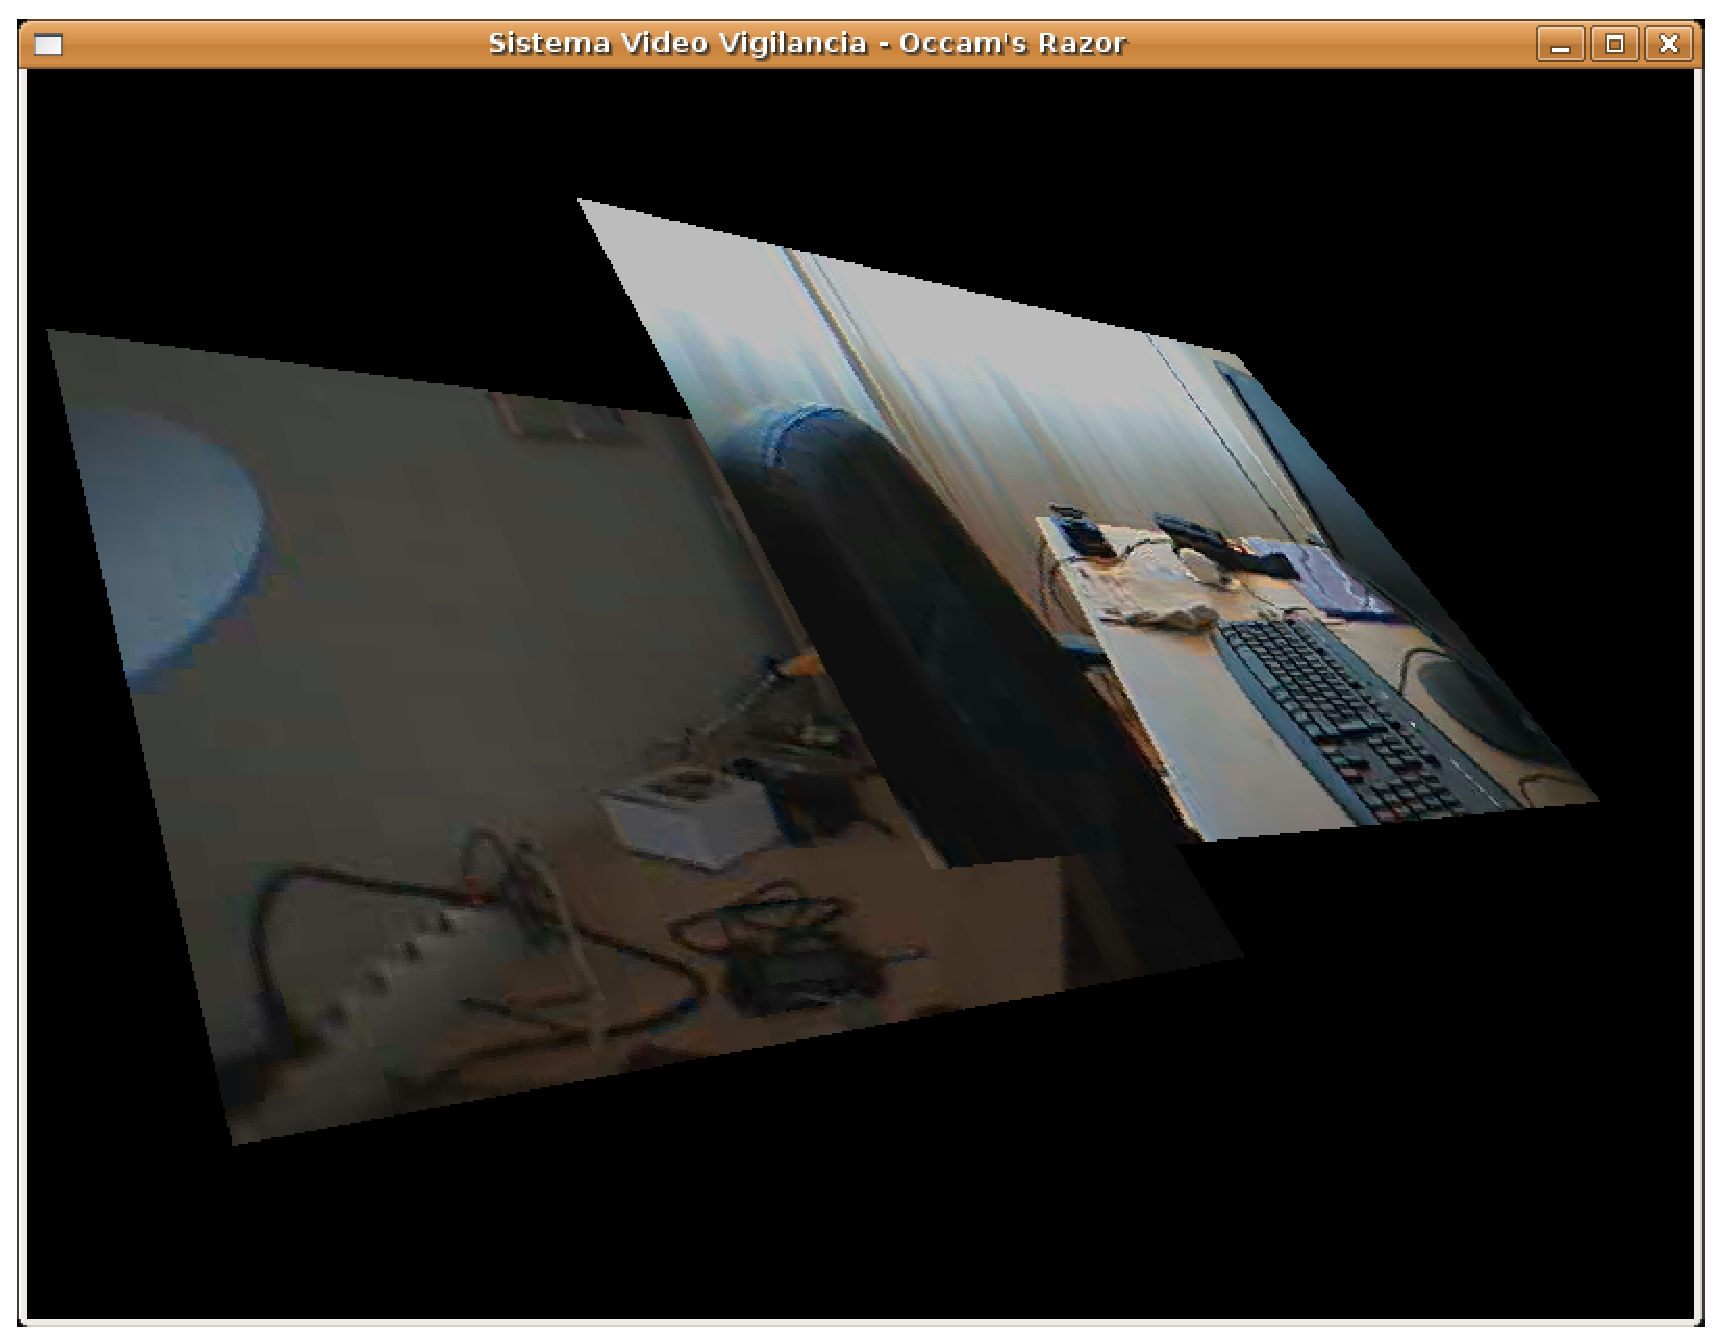
\includegraphics[height=5.5cm,angle=0]{images/murapido/shot06.eps}

{\footnotesize\bf Jugando un poco podemos conseguir efectos m�s interesantes}

\end{figure}

\bigskip

\begin{multicols}{2}

\sectiontext{white}{black}{GENERANDO LAS IM�GENES}

En la secci�n anterior hemos visto como componer la escena OpenGL,
pero todav�a no os hemos contado como visualizar realmente las
im�genes.

Esto se puede hacer manipulando el frame buffer directamente, pero
nosotros hemos elegido hacerlo utilizando texturas. El uso de texturas
proporciona dos ventajas frente a escribir los datos directamente en
el frame buffer: La primera es que la t�cnica es m�s r�pida, y la
segunda es que si queremos cambiar el tama�o de la imagen, OpenGL
realizar� la interpolaci�n por nosotros.

\begin{entradilla}
{\em {\color{introcolor} Utilizaremos texturas} para la visualizaci�n
del video en directo}
\end{entradilla}

As�, el m�todo consiste en lo siguiente. Primero generamos e
inicializamos una textura por cada imagen que queremos
mostrar. Utilizamos las im�genes capturadas para inicializar los datos
de la textura y finalmente, dibujamos un cuadro sobre el que mapeamos
esta textura. 

Si hab�is seguido los comentarios del programa principal, recordar�is
que se nos han quedado tres funciones en el tintero. La primera se
utiliza en la funci�n main y se llama \verb!init_texture!. La segunda se
utiliza cuando capturamos nuestras im�genes y se llama,
\verb!change_texture!. Y finalmente, la �ltima la acabamos de ver en la
secci�n anterior y se llama \verb!square_texture!. 

\sectiontext{white}{black}{INICIALIZANDO LAS TEXTURAS}

La funci�n \verb!init_texture! se encarga de la inicializaci�n de las
texturas. La inicializaci�n consiste en decirle a OpenGL que le de
``nombre'' a las texturas que vamos a utilizar y que inicialice sus
atributos. Recordad que aunque nosotros vamos a utilizar la textura
para visualizar una imagen, las texturas se utilizan sobre modelos 3D
para darles mayor realismo. Cuando hacemos esto �ltimo todos estos
par�metros toman mucho m�s sentido.

La funci�n \verb!init_texture! es la encargada de hacer esto. La hemos
intentado reducir a la m�nima expresi�n, y el resultado es este:

\lstset{language=C,frame=tb,framesep=5pt,basicstyle=\scriptsize}   
\begin{lstlisting}
#define MAX_TEXTURE 4

static GLuint texid[MAX_TEXTURE];

void init_texture (int w, int h)
{
  int     i;

  /* Almacenamos las dimensiones para m�s tarde*/    
  tex_w = w;
  tex_h = h;

  /* Genera "Nombres" OpenGL para las texturas */
  glGenTextures (MAX_TEXTURE, &texid);

  for (i = 0; i < MAX_TEXTURE; i++)
    {
      glBindTexture (GL_TEXTURE_2D, texid[i]);
  
      /* Define el tipo de interpolaci�n */
      /* Para ampliar la textura*/
      glTexParameteri (GL_TEXTURE_2D, 
                       GL_TEXTURE_MAG_FILTER, 
                       GL_NEAREST);

      /* Para disminuir la textura*/
      glTexParameteri (GL_TEXTURE_2D, 
                       GL_TEXTURE_MIN_FILTER, 
                       GL_NEAREST);
      
      /* Inicializa los datos de la textura */
      glTexImage2D (GL_TEXTURE_2D, 0, GL_RGBA8, 
                    w, h, 0, GL_RGB, 
                    GL_UNSIGNED_BYTE, NULL);
    }    
    
}
\end{lstlisting}

Nuestro m�s-que-b�sico gestor de texturas es capaz de manejar un
m�ximo de cuatro de ellas y almacena sus identificadores en una variable
global del m�dulo llamada \verb!texid!. 

Lo primero que hacemos es decirle a OpenGL que necesitamos 
cuatro texturas y que nos almacene los identificadores en la matriz
\verb!texid!. A continuaci�n, tenemos que inicializar cada una de ellas. 

Aqu� podemos configurar un mont�n de par�metros de la textura, pero
nosotros solo hemos dejado uno de ellos. Obviamente la forma de
configurar los par�metros de las texturas es utilizando la funci�n
\verb!glTexParameteri!... est� claro no? :).


%%%%%%%%%%%%%%%%%%%%%%%%%%%%%%%%%%%%%%%%%%%%%%%%%%%%%%%%%%%%%%%%%%%
\ebOpage{introcolor}{0.25}{M� R�PIDO}

Los dos par�metros que hemos usado le dicen a OpenGL que filtro
utilizar cuando tiene que ampliar la textura o hacerla m�s
peque�a. Nosotros hemos utilizado el filtro "del vecino m�s cercano",
que en principio es el m�s r�pido, pero pod�is utilizar interpolaci�n
lineal, mejorando la calidad del zoom de vuestras aplicaciones,
simplemente cambiando este par�metro de \verb!GL_NEAREST! a \verb!GL_LINEAR!.

Finalmente, la funci�n \verb!glTexImage2D! es la que nos permite definir el
formato de los datos de imagen que vamos a pasar a OpenGL. Como pod�is
ver los datos se corresponden con los que hemos utilizado todo el
tiempo, ancho, alto y formato (RGB 24bits). El �ltimo par�metro es un
puntero a los datos de imagen 
a almacenar en la textura. Nosotros haremos esto en otra funci�n y por
eso pasamos el valor NULL.

\begin{entradilla}
{\em OpenGL nos permite {\color{introcolor} suavizar las im�genes por
Hardware} con un simple par�metro}
\end{entradilla}

Algunos comentarios dependientes de la implementaci�n concreta de
OpenGL que est�is usando: El primero es que muchas implementaciones
viejas necesitan que los dimensiones de las texturas (ancho y alto)
sean potencias de dos. Si este es vuestro caso (obtendr�ais una imagen
blanca en lugar de la imagen de la c�mara), en la funci�n de
inicializaci�n tendr�is que aproximar las dimensiones de vuestras
im�genes a los valores correctos.

El otro comentario, es que algunas implementaciones de OpenGL,
soportan el formato de texturas GL\_BGR. Si record�is, nuestro
dispositivo V4L, nos devolv�a los valores en este formato, y tuvimos
que a�adir un peque�o bucle para ordenarlos antes de envi�rselos a
OpenGL.... Pues quiz�s os lo pod�is ahorrar.

\sectiontext{white}{black}{CAMBIANDO LOS DATOS DE LA TEXTURA}

Cada vez que capturamos una imagen, tenemos que actualizar nuestra
textura. Esto lo hacemos con la funci�n \verb!change_texture! que pod�is ver
a continuaci�n.

\columnbreak

\lstset{language=C,frame=tb,framesep=5pt,basicstyle=\scriptsize}   
\begin{lstlisting}
void change_texture (int id, char *in_data)
{
  glBindTexture (GL_TEXTURE_2D, texid[id]);
  
  glTexSubImage2D (GL_TEXTURE_2D, 0, 0, 0, 
  tex_w, tex_h, GL_RGB, GL_UNSIGNED_BYTE, in_data);
  
}
\end{lstlisting}

Esta es sencilla no?. La funci�n \verb!glBindTexture! le dice a OpenGL que
textura queremos utilizar. S�, es la misma que utilizamos para
configurar la textura tras su creaci�n. El �ndice que pasamos como primer par�metro
nos permite obtener el identificador OpenGL de la textura que nos
interesa.

Una vez seleccionada la textura, utilizamos la funci�n
\verb!glTexSubImage2D!, que es exactamente igual a la funci�n \verb!glTexImage2D!
que utilizamos en la inicializaci�n, pero �sta nos permite actualizar solo
una parte de la textura. 

Esta funci�n es en principio m�s r�pida, y adem�s funcionar� si
nuestra implementaci�n OpenGL tiene la limitaci�n de las potencias de
2, ya que nos permitir� actualizar la parte de la textura que realmente
utilizamos.

\sectiontext{white}{black}{PINTANDO LAS IM�GENES}

Ya estamos en condiciones de pintar la imagen. Como comentamos, lo que
vamos a hacer es pintar un cuadro sobre el que mapearemos una
textura. Esta es la forma de hacerlo.

\lstset{language=C,frame=tb,framesep=5pt,basicstyle=\scriptsize}   
\begin{lstlisting}
void square_texture (int id)
{
 
  glBindTexture (GL_TEXTURE_2D, texid[id]);
  
  glBegin (GL_QUADS);
  glTexCoord2f (0.0, 0.0); glVertex2f (0.0, 1.0);
  glTexCoord2f (0.0, 1.0); glVertex2f (0.0, 0.0);
  glTexCoord2f (1.0, 1.0); glVertex2f (1.0, 0.0);
  glTexCoord2f (1.0, 0.0); glVertex2f (1.0, 1.0);
  glEnd ();

}
\end{lstlisting}

Lo primero que hace la funci�n, es seleccionar la textura que vamos a
mapear, con la habitual llamada a \verb!glBindTexture!. A continuaci�n,
dibujaremos el cuadrado, para lo que tendremos que decirle a OpenGL
cuales ser�n las coordenadas de sus v�rtices, y que ``punto'' de la
textura queremos asociar a cada uno de ellos.


\end{multicols}

\begin{figure}[ht]
\centering
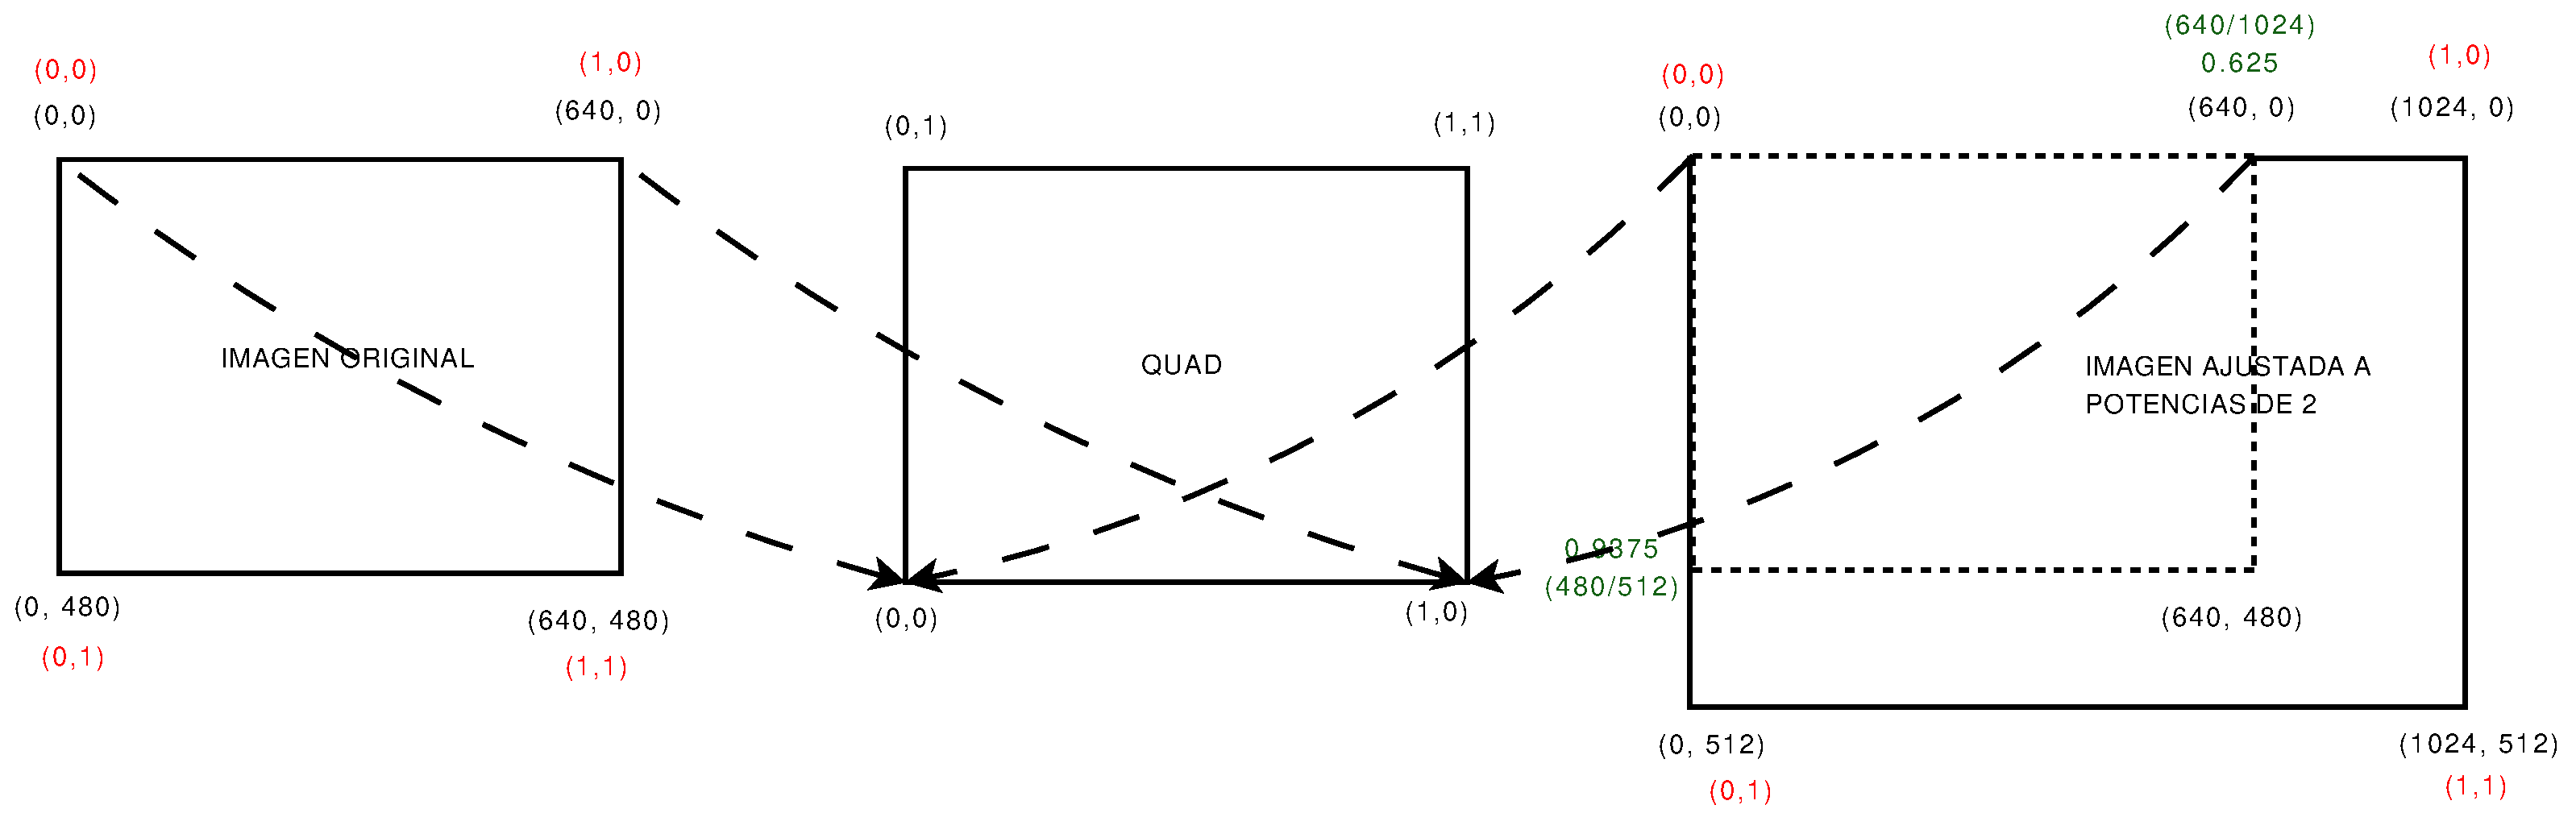
\includegraphics[height=4.0cm,angle=0]{images/murapido/mapeado_textura.eps}

{\footnotesize\bf Transformaciones de coordenadas para mapeado de texturas}
\end{figure}


\clearpage
\pagebreak


%%%%%%%%%%%%%%%%%%%%%%%%%%%%%%%%%%%%%%%%%%%%%%%%%%%%%%%%%%%%%%%%%%%
\bOpage{introcolor}{0.25}{M� R�PIDO}

La funci�n \verb!glTexCoord2f!, nos permite seleccionar un punto dentro de la
textura. El 0,0 ser� el punto inicial de nuestra imagen, y el 1,1 se
corresponder� con la esquina inferior derecha. Si os fij�is, las
coordenadas de la textura y del v�rtice del cuadro no se
corresponden. Esto sucede porque el sistema de coordenadas OpenGL
asigna el origen a la esquina inferior izquierda y la imagen que nos
devuelve nuestro dispositivo de captura, est� definida respecto a la
esquina superior izquierda. 

\begin{entradilla}
{\em Para utilizar {\color{introcolor} nuestra imagen como textura} es necesario realizar
algunas transformaciones}
\end{entradilla}

Observad que si hab�is modificado el programa para utilizar texturas
con dimensiones m�ltiplos de potencias de 2, la parte de la textura
que contiene la imagen no se corresponde con el tama�o de la textura
(hay una parte negra a la derecha). En ese caso, tendr�is que
sustituir el valor 1.0 en \verb!glTexCoord2f!, por el valor apropiado, que
depender� del tama�o de vuestra imagen.

Finalmente, �record�is el escalado especial de la coordenada Y en la
funci�n que dibuja la escena?. Como pod�is ver aqu�, lo que estamos
dibujando es un cuadrado. Si en lugar de un cuadrado, dibuj�ramos el
rect�ngulo con el aspecto correcto, no ser�a necesario escalar la
coordenada Y de forma especial... La mejor opci�n depender� de cada
aplicaci�n. 

\sectiontext{white}{black}{INICIALIZACI�N DE OPENGL}

Para terminar con todo lo relacionado con la visualizaci�n, tenemos
que comentar una �ltima funci�n, \verb!gfx_init!. Esta funci�n se encarga de
inicializar OpenGL, y en general contiene comandos OpenGL que
solamente es necesario ejecutar una vez.

En nuestro caso la funci�n es muy sencilla.

\lstset{language=C,frame=tb,framesep=5pt,basicstyle=\scriptsize}   
\begin{lstlisting}
void gfx_init (void)
{
  glClearColor (0, 0, 0, 0);
  glEnable (GL_DEPTH_TEST);
  glEnable (GL_TEXTURE_2D);
}
\end{lstlisting}

El primer comando define el color de fondo a utilizar cuando borremos
los buffers de color (la imagen en la ventana), utilizando la funci�n
\verb!glClear! (la primera llamada en \verb!gfx_pinta!).

Las otras dos funciones permiten activar, respectivamente, el uso del
z-buffer y el de las texturas 2D. Tened en cuenta que antes de
ejecutar ninguna de las funciones relacionadas con la manipulaci�n de
las texturas que acabamos de ver, necesitamos ejecutar esta funci�n
para activar el uso de texturas 2D. Si no lo hacemos obtendremos una
imagen vac�a.

El uso de z-buffer es necesario si las im�genes se van a solapar de
alguna manera en la escena. Si no activamos el z-buffer, las im�genes
se visualizar�n en el orden en el que las pintemos en nuestro
programa, independientemente de su posici�n real en el espacio 3D. 

Si no quer�is hacer filigranas con las texturas y vuestras im�genes
van a aparecer en una posici�n fija en la pantalla (lo usual en un
sistema de v�deo vigilancia), pod�is desactivar el z-buffer, ahorrando
memoria y trabajo a vuestra tarjeta gr�fica. En este mismo caso,
probablemente os interese m�s utilizar una proyecci�n ortogr�fica que
la perspectiva que estamos utilizando... solo estamos dando pistas...

\sectiontext{white}{black}{VOLCANDO IM�GENES}

El �ltimo elemento que nos queda es la funci�n para volcar las
im�genes capturadas al disco. Desde el punto de vista del almacenaje
nos interesa utilizar un formato comprimido, pero antes os vamos a
comentar como utilizar el formato Netpbm, que es tremendamente
sencillo y si lo utilizamos junto con zlib, nos puede solucionar el
problema m� r�pido.

Aqu� ten�is la funci�n para grabar vuestras im�genes:

\lstset{language=C,frame=tb,framesep=5pt,basicstyle=\scriptsize}   
\begin{lstlisting}
int write_image (char *fname, char*data)
{
  FILE *f;

  f = fopen (fname, "wb");
  fprintf (f, "P6\n#Occam's Razor "
              "Video Vigilancia\n"
              "%d %d\n%d\n",
	   img_w, img_h, 255);
  fwrite (data, img_size, 1, f);
  fclose (f);
}
\end{lstlisting}

M�s r�pido no se puede XD. El formato ppm, utiliza una sencilla
cabecera ASCII, en la que se indican las dimensiones de la imagen y su
profundidad de color (el valor 255 indica 8 bits por componente). A
continuaci�n escribimos los datos y listo.

\begin{entradilla}
{\em El {\color{introcolor} formato PPM} es muy conveniente para volcar im�genes de forma sencilla}
\end{entradilla}

El problema de PPM es que los datos no se comprimen en absoluto. Cada
imagen captura por nuestra aplicaci�n ocupa unos 900Kb. La misma
imagen en formato jpg ocupa unos 19Kb, y por eso os vamos a contar
como usar este formato.

En la secci�n Ratas de Biblioteca de el n�mero 1 de Occam's Razor, os
cont�bamos como utilizar zlib para almacenar ficheros. Alguien quiere
modificar la funci�n de arriba y ver cuanto puede comprimir nuestras
im�genes zlib?. Esperamos vuestros resultados ;)


%%%%%%%%%%%%%%%%%%%%%%%%%%%%%%%%%%%%%%%%%%%%%%%%%%%%%%%%%%%%%%%%%%%
\ebOpage{introcolor}{0.25}{M� R�PIDO}

\sectiontext{white}{black}{USANDO JPEG}

Al principio del art�culo os dec�amos que �bamos a utilizar libjpeg
para almacenar las imagenes, y como lo prometido es deuda, aqu� ten�is
la funci�n para almacenar una imagen en formato JPEG en el disco:

\lstset{language=C,frame=tb,framesep=5pt,basicstyle=\scriptsize}   
\begin{lstlisting}
#include <jpeglib.h>

int color_space = JCS_RGB; 
/* JCS_GRAYSCALE para nivels de gris */

int 
write_jpeg_file(char *filename, char *buffer, 
                int w, int h, int bpp )
{
  struct jpeg_compress_struct cinfo;
  struct jpeg_error_mgr jerr;
  
  JSAMPROW row_pointer[1];
  FILE *outfile = fopen( filename, "wb" );
  
  if ( !outfile )
    {
      printf("Error opening output jpeg " 
             "file %s\n!", filename );
      return -1;
    }

  cinfo.err = jpeg_std_error( &jerr );
  jpeg_create_compress(&cinfo);
  jpeg_stdio_dest(&cinfo, outfile);
  
  cinfo.image_width = w;
  cinfo.image_height = h;
  cinfo.input_components = bpp;
  cinfo.in_color_space = color_space;

  jpeg_set_defaults( &cinfo );

  jpeg_start_compress( &cinfo, TRUE );

  while(cinfo.next_scanline<cinfo.image_height)
    {
      row_pointer[0]=&buffer[cinfo.next_scanline* 
                           cinfo.image_width*  
                           cinfo.input_components];
      jpeg_write_scanlines( &cinfo, row_pointer, 1);
    }
  /* similar to read file, clean up after 
     we're done compressing */
  jpeg_finish_compress( &cinfo );
  jpeg_destroy_compress( &cinfo );
  fclose( outfile );
  return 1;
}
\end{lstlisting}

Bueno, esta funci�n la pod�is encontrar en los ejemplos que se
distribuyen con el c�digo fuente de libjpeg. En el mismo fichero
pod�is encontrar la funci�n para leer un fichero jpeg del disco.



El c�digo es autoexplicativo, y adem�s, as� es como funciona la
librer�a, no hay mucho que rascar. 

\begin{entradilla}
{\em {\color{introcolor}libjpeg} nos permite grabar {\color{introcolor}im�genes en formato JPEG} de forma sencilla}
\end{entradilla}

Con esta funci�n podremos almacenar
las im�genes capturadas en formato jpeg. Esto es m�s o menos
equivalente a almacenar la secuencia de video en formato MJPEG, lo que
no est� nada mal.

\sectiontext{white}{black}{A JUGAR!}

Bueno, este art�culo ha sido un poco largo, pero hemos tratado un
mont�n de cosas distintas que nos dan mucho juego. Aqu� van algunas
propuestas:

\begin{itemize}
\item A�adir soporte de red a la aplicaci�n. Con lo que os hemos contado
  en los n�meros anteriores de Occam's Razor, en esta misma secci�n,
  eso deber�a estar {\em chupao}!
\item Captura de v�deos panor�micos. Utilizando varias c�maras, podemos
  modificar nuestro programa para poder generar v�deos panor�micos,
  utilizando un par de webcams :).
\item Vigilando en est�reo?. Ten�is unas gafas de esas rojas y
  azules?. Sab�is lo que es un anaglifo? (buscad Anaglifo en la
  wikipedia :)). Sab�is que con el c�digo de este art�culo, pod�is
  generar un anaglifo modificando una sola l�nea del c�digo!!!!
  (bueno, y colocando las c�maras correctamente).
\item Grabar la secuencia de v�deo en formato AVI, MPEG o lo que os
  apetezca (pista... ffmpeg).
\end{itemize}

Y cualquier otra cosa que se os ocurra. No os olvid�is de enviarnos
vuestros experimentos!!. Esta vez hay cosas de sobra para
jugar!. Hasta el pr�ximo n�mero. \EOP


%% Tabla de recursos en internet 

\end{multicols}

{\colorbox{introcolor}{
\begin{minipage}{0.98\linewidth}
{\textsf
{\color{white}{\Large RECURSOS}}

\footnotesize

\medskip

{\textsf{Driver GSPCA y Spcaview}}

{\footnotesize\url{http://mxhaard.free.fr/download.html}}

\medskip

{\textsf{FAQ de motion con mucha informaci�n interesante}}

{\footnotesize\url{http://www.lavrsen.dk/twiki/bin/view/Motion/FrequentlyAskedQuestions}}
\medskip

{\textsf{Tutoriales y ejemplos OpenGL}}

{\footnotesize\url{http://www.opengl.org/code/}}
\medskip

{\textsf{Formato PPM}}

{\footnotesize\url{http://netpbm.sourceforge.net/doc/ppm.html}}

\medskip

{\textsf{Libjpeg a trav�s de la wikipedia}}

{\footnotesize\url{http://en.wikipedia.org/wiki/Libjpeg}}

\medskip


{\textbf{\textsf{Para los que quieran jugar}}}

{\textsf{Anaglifos}}

{\footnotesize\url{http://es.wikipedia.org/wiki/Anaglifo}}


{\textsf{P�gina web de FFMPEG}}

{\footnotesize\url{http://en.wikipedia.org/wiki/Libjpeg}}

\medskip


\normalsize
}
\end{minipage}
}}


\clearpage
\pagebreak

 

% Este fichero es parte del N�mero 4 de la Revista Occam's Razor
% Revista Occam's Razor N�mero 4
%
% (c)  2009, The Occam's Razor Team
%
% Esta obra est� bajo una licencia Reconocimiento 3.0 Espa�a de
% Creative Commons. Para ver una copia de esta licencia, visite
% http://creativecommons.org/licenses/by/3.0/es/ o envie una carta a
% Creative Commons, 171 Second Street, Suite 300, San Francisco,
% California 94105, USA. 

% Seccion Historia
%

\rput(8.5,-4.3){\resizebox{19cm}{!}{{\epsfbox{images/historia/historia.eps}}}}

% -------------------------------------------------
% Cabecera special... solo imagen

\vspace{7.5cm}

% -------------------------------------------------

\begin{multicols}{2}

% Introducci�n
\intro{introcolor}{C}{uando la direcci�n de la revista me propuso
escribir este art�culo, me di cuenta de que sin pretenderlo me he
convertido en una especie de historiador tecnol�gico
aficionado. Aprovecho para recomendaros (si no los hab�is le�do ya)
mis anteriores art�culos ``Mi Historia de las Telecomunicaciones'' y
``El tel�grafo de Gauss'', ya sab�is que nunca puedo resistirme a
hacer un poco de autobombo. En fin, ya que este n�mero va dedicado a
las tecnolog�as de seguridad resulta muy propio un art�culo sobre la
historia de la criptograf�a. La criptograf�a es la ciencia (o la
t�cnica) de ``poner en clave'' mensajes de forma que un esp�a que
logre interceptarlos no pueda entenderlos pero aquellos que conozcan
la clave (o claves) adecuada(s) logren f�cilmente recuperar la
informaci�n inicial. Como veremos, la criptograf�a existe desde
tiempos muy antiguos, aunque ha sido la llegada de los ordenadores la
que ha logrado crear sistemas realmente potentes y seguros. 
}

\vspace{2mm}

% Cuerpo del art�culo

Si me permit�s repetirme un poco volveremos a la definici�n. El
t�rmino {\em criptograf�a} procede de la uni�n de dos palabras griegas:
krypto (ocultar) y graphos (escribir). Se trata por tanto de
``escritura oculta''... es decir: la criptograf�a es un conjunto de
t�cnicas que permiten poner un mensaje cualquiera en un formato
ininteligible para todos, excepto para aquellos que poseen una
informaci�n adicional (clave). Por supuesto, la clave es una
informaci�n necesaria para realizar el proceso de cifrado (encriptado
o puesta en clave) y tambi�n para el proceso de descifrado. Seg�n el
algoritmo empleado, la clave puede ser un n�mero, una letra, un
conjunto de bits o, incluso, cosas m�s raras como una tabla de
s�mbolos. 




Una suposici�n fundamental en todos los estudios criptogr�ficos es que la seguridad se debe basar en el secreto de la clave, nunca en el secreto del algoritmo. Los algoritmos de cifrado deben ser p�blicos. Un sistema que se base en el secreto del algoritmo quedar� comprometido si se descubre �ste. Sin embargo, si se descubre una clave, podremos seguir operando el sistema cambi�ndola.

Para terminar la introducci�n veremos un poco de terminolog�a sobre el cifrado, a saber:

\begin{itemize}
\item {\bf Mensaje llano}: es el mensaje inicial, antes de ser cifrado, por tanto todav�a legible.
\item {\bf Criptograma}: mensaje una vez cifrado.
\item {\bf Criptoan�lisis}: son las operaciones que realiza un esp�a para intentar averiguar el mensaje llano. 

Normalmente, se supone que el esp�a conoce el algoritmo pero no la clave. El criptoan�lisis es diferente si el esp�a s�lo dispone de un criptograma, de varios o dispone de texto seleccionado (criptogramas para los que conoce el texto llano). Esta �ltima es la situaci�n m�s favorable para el ataque. Pensad que hay un criptoan�lisis que nunca falla: probar todas las claves posibles (m�todo de la fuerza bruta). Un buen algoritmo de cifrado debe estar pensado para que el �nico ataque posible sea la fuerza bruta y, adem�s, para que este ataque no sea viable. Para evitar la fuerza bruta, debe haber muchas claves posibles (longitud de clave de muchos bits) de forma que comprobar todas consuma una cantidad de tiempo excesiva (del orden de siglos).

\end{itemize}


\begin{entradilla}
{\em Criptograf�a significa literalmente {\color{introcolor} escritura
oculta}}
\end{entradilla}


{\colorbox{excolor}{
\begin{minipage}{0.98\linewidth}
Como sabr�is (creo que es una de las cosas que ense�a esta revista), la mente humana es infinita y hasta ha habido estudios matem�ticos sobre c�mo crear un algoritmo matem�ticamente seguro ante la fuerza bruta. Como no, se debe al creador de la teor�a de la informaci�n (Claude E. Shannon).
�C�mo es posible esto? -os preguntar�is. Si se puede descifrar sabiendo la clave, cualquiera puede ponerse a probar claves: {\bf CIERTO}.

\end{minipage}
}}

\ebOpage{introcolor}{0.25}{HISTORIA}

{\colorbox{excolor}{
\begin{minipage}{0.98\linewidth}
El problema ``no resuelto'' es: �C�mo hace el criptoanalista para saber qu� clave es la buena, si no conoce el texto en llano? Nuestro malvado esp�a se tiene que basar en tomar una decisi�n binaria ante cada prueba: �El mensaje descifrado tiene sentido o no? Si un algoritmo es atacado por fuerza bruta y obtenemos varios mensajes coherentes probando claves distintas, no sabremos cu�l de ellas es. Realmente, si el esp�a puede reducir la inc�gnita sobre la clave, en el pr�ximo criptograma que analice tendr� menos claves que probar.
Por otra parte, la coherencia del mensaje es algo totalmente dependiente del tipo de mensaje. Si sabemos que son im�genes JPEG deben cumplir un formato y adem�s salir algo con sentido al representarlas. �Algo con sentido? algunas im�genes microsc�picas pueden no parecer con mucho sentido

\end{minipage}
}}

\bigskip

\sectiontext{white}{black}{CIFRADOS DE SUSTITUCI�N}

La t�cnica de cifrado m�s antigua es la de sustituci�n. Como su nombre indica, consiste en sustituir cada s�mbolo (letra) del alfabeto con el que representamos nuestros mensajes por otro s�mbolo de otro alfabeto (o del mismo).

El primer m�todo sistem�tico de cifrado del que se tiene noticia fue
utilizado por los militares romanos y se conoce todav�a hoy como
``Cifrado de C�sar''. Se le llama as� porque se encontraron documentos
cifrados con esta t�cnica por Julio C�sar y por su heredero Augusto;
sin embargo, no est� demostrado que C�sar fuera el primero en
emplearlo.


\begin{entradilla}
{\em El {\color{introcolor} cifrado de C�sar} fu� el primer sistema de
cifrado sistem�tico que se conoce.}
\end{entradilla}

El cifrado de C�sar se basa en una sustituci�n de las letras del alfabeto latino (el nuestro) por ellas mismas seg�n una clave que no es m�s que un desplazamiento. Esto es: si la clave es +1 cada letra se sustituye por la siguiente del alfabeto, en vez de C�SAR (ignorando el acento) escribir�amos DFTBS. N�tese que en aquella �poca el cifrado se realizaba de ``memoria''. L�gicamente, el desplazamiento es circular: despu�s de la Z viene la A. Tambi�n son posibles los desplazamientos negativos aunque -1 ser�a equivalente a 25 (si hay 26 letras). N�tese que para N letras en el alfabeto hay N-1 posibles claves y un desplazamiento d es equivalente al d+N. El n�mero tan reducido de claves se debe a que estamos conservando el orden de las letras. Si consideramos sustituir el alfabeto latino por �l mismo sin ninguna restricci�n el n�mero de claves posibles ser� N!

\begin{entradilla}
{\em El {\color{introcolor}cryptoan�lisis de la sustituci�n} es muy simple.}
\end{entradilla}

Ya es un t�pico pero es este momento es inevitable recordar que en el nombre de la computadora de la pel�cula 2001: ``HAL'' hab�a un mensaje cifrado. �Alguien no lo sab�a? Pistas: el m�todo empleado ya lo hemos comentado en este art�culo y el mensaje llano tiene algo que ver con la inform�tica.

Otro tipo de cifrados de sustituci�n son los que inventan nuevos alfabetos donde cada s�mbolo representa una letra. La clave pasa por conocer la correspondencia entre letras y s�mbolos. Realmente estos m�todos no son m�s seguros que una sustituci�n de las letras est�ndar por ellas mismas. Sigue habiendo N! ordenaciones.

El criptoan�lisis de la sustituci�n es muy simple y la manera m�s gratificante de aprenderlo ser�a leer ``El Escarabajo de Oro''. En este relato (nunca he sabido si es un cuento largo o una novela corta) los protagonistas descifran un mensaje pirata (con alfabeto de s�mbolos inventados mezclados con n�meros y signos de puntuaci�n). La t�cnica que usan es probabil�stica: ya que la E es la letra m�s usada del ingl�s debe ser la que corresponde con el s�mbolo m�s repetido. Conociendo la frecuencia de las letras en el idioma podemos hacer suposiciones de este tipo sobre dos o tres caracteres e intentar descubrir alguno m�s. Para eso ayudan mucho las part�culas de cada idioma, en el ejemplo del escarabajo de oro logran descifrar la T y la E y ven muchas veces la palabra T4E, con lo que ``4'' debe ser la H (recu�rdese que era un mensaje en ingl�s). �Qui�n es el autor de este relato? Se trata de un novelista norteamericano genial aunque de vida algo atormentada: Edgar Allan Poe.

Por supuesto que si sabemos que es un cifrado C�sar la fuerza bruta nos puede ayudar (el n�mero de claves es rid�culamente bajo). Ojo... no hay constancia de que ning�n enemigo lograra, en su �poca, descifrar los mensajes cifrados por C�sar por lo que confirmamos (por si no lo sab�amos) que el valor de una tecnolog�a es siempre relativo a su �poca (tambi�n hay que decir que la mayor�a de esos enemigos no sab�an leer).

\end{multicols}

{\colorbox{introcolor}{
\begin{minipage}{0.98\linewidth}
{\large\textbf{La criptograf�a como disciplina matem�tica}}

\medskip

Realmente la criptograf�a puede verse como una parte de las matem�ticas dedicada a crear funciones inestables. Un algoritmo criptogr�fico es una funci�n que opera con dos variables: el mensaje llano y la clave para obtener un resultado: el criptograma. Esa funci�n debe ser biyectiva, esto es inversible ya que debe existir una funci�n inversa que a partir del criptograma y la clave permita obtener de nuevo el mensaje llano.
Para que una funci�n ``cifre'' debe ser inestable, esto es: al modificar muy poco el mensaje o la clave el criptograma debe variar mucho... eso asegura que es dif�cil de invertir sin conocer la clave ya que no podemos hacer aproximaciones sucesivas.

\end{minipage}
}}

\clearpage
\pagebreak

\msection{introcolor}{black}{0.25}{HISTORIA}

\begin{figure}[ht]
\centering
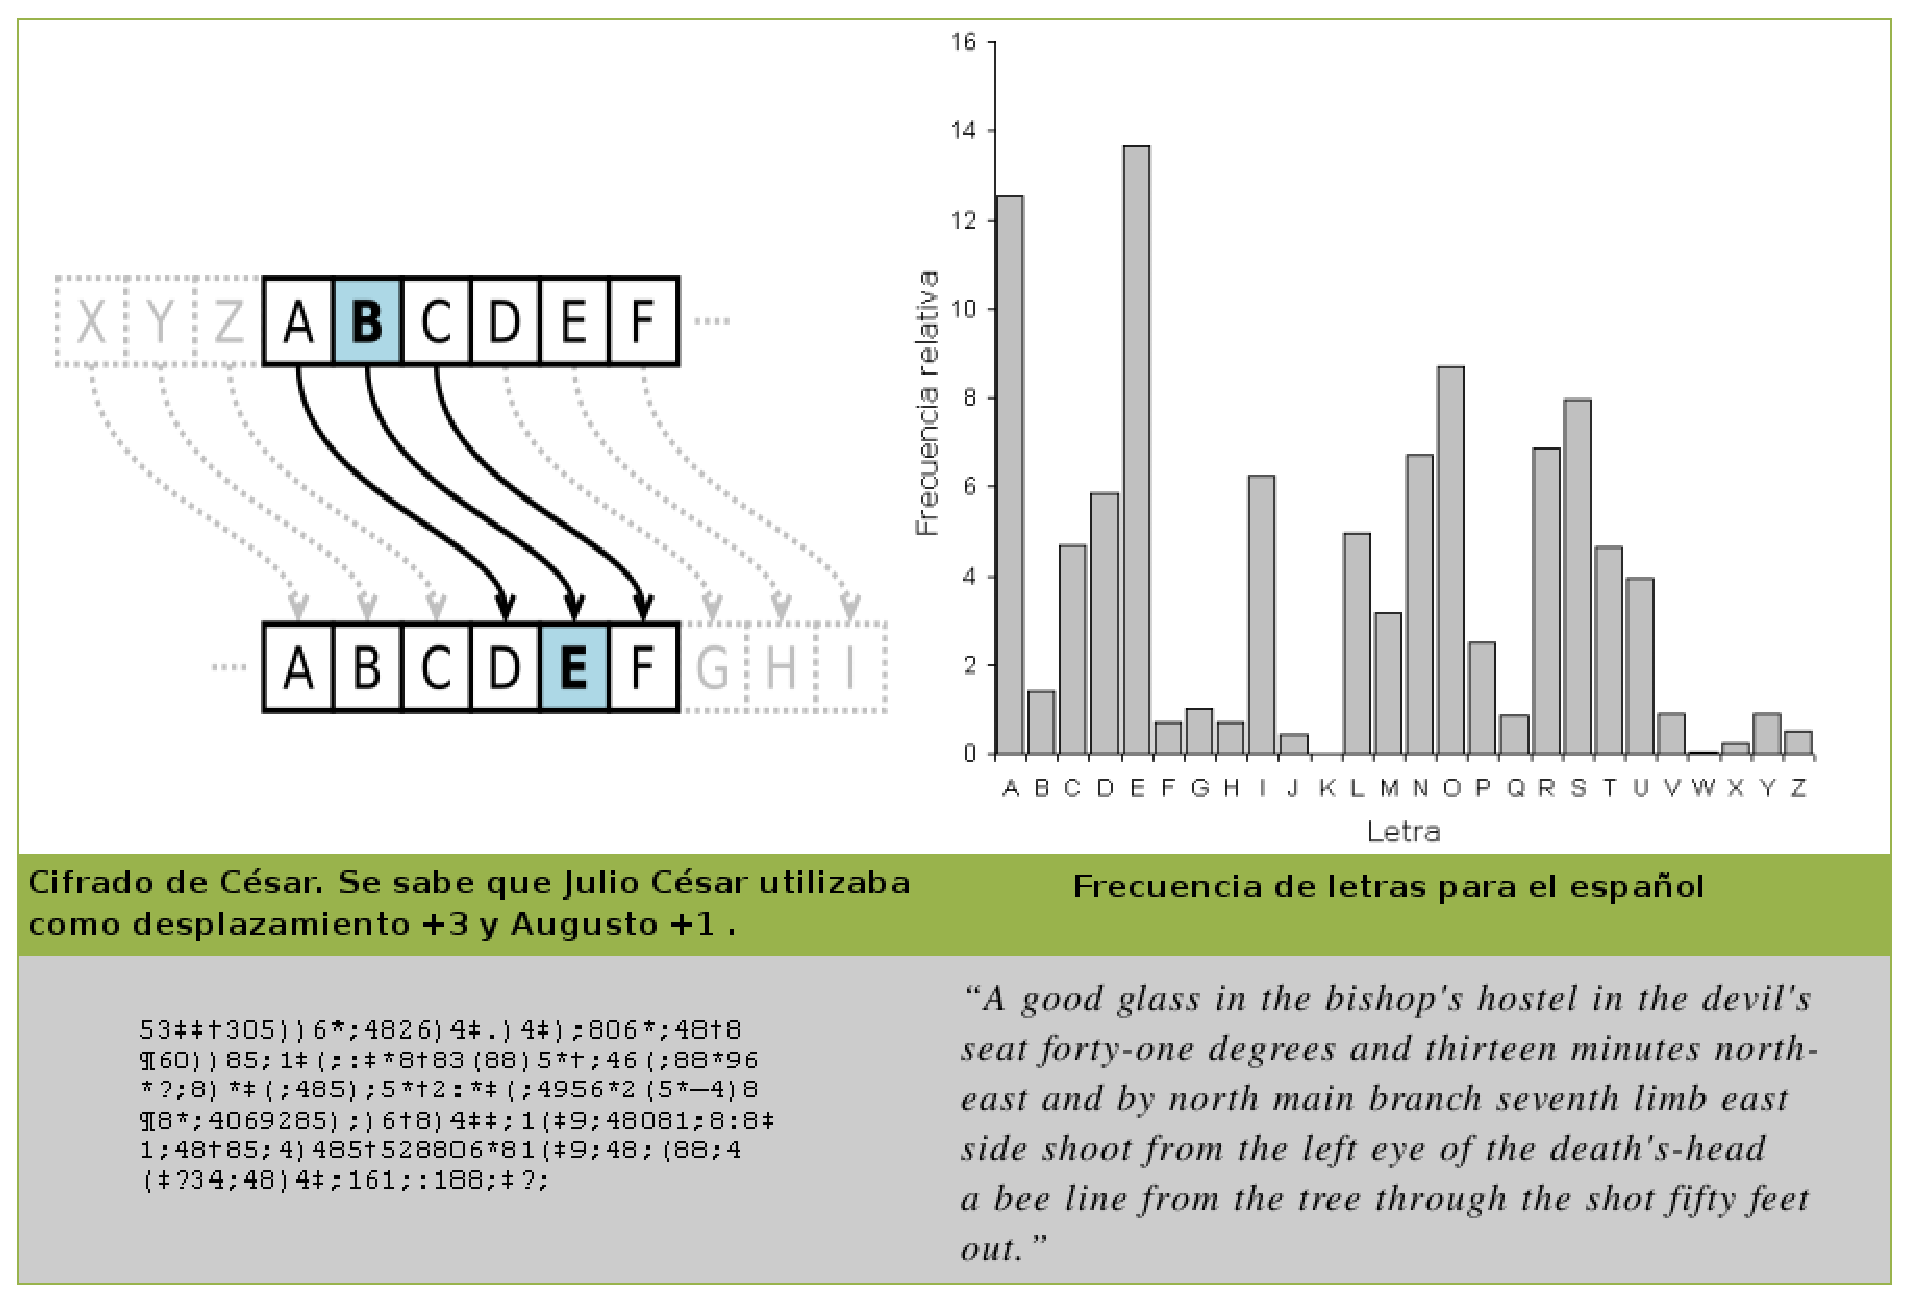
\includegraphics[height=11.0cm,angle=0]{images/historia/criptografia-image2.eps}

{\footnotesize\bf Criptograma de ``El Escarabajo de Oro'' y su texto llano una vez descifrado. N�tese que se eliminan los espacios para lograr una mayor confusi�n del lector.
.}
\end{figure}

\bigskip

\begin{multicols}{2}

Otro m�todo de sustituci�n muy utilizado hasta el siglo XIX (y muy seguro en aquella �poca) es el m�todo de Vigen�re. Realmente, se trata de una mejora del m�todo de C�sar. La idea es muy simple... definamos M claves para el m�todo de C�sar (M n�meros entre 1 y 25 para un alfabeto de 26 letras). Si aplicamos el cifrado de C�sar con la primera clave a la primera letra, el mismo m�todo a la segunda letra con la segunda clave... tendremos un cifrado C�sar con clave variable. A partir de M aplicaciones volvemos a la primera clave.

El acierto de este m�todo es que una misma letra ser� cifrada de forma diferente aunque aparezca muchas veces. Si cada clave C�sar, se representa por una letra (donde la A es el desplazamiento 0 y la Z el 26) la clave completa (M letras) se podr� escribir como una palabra. No hay longitud m�nima ni m�xima. De hecho, la longitud de la clave es el gran secreto del m�todo.

\begin{entradilla}
{\em El {\color{introcolor} cifrado de Vigen�re} realiza una sustituci�n polialfab�tica.}
\end{entradilla}

Este m�todo se consider� invulnerable hasta que el militar prusiano Friedrich Kasiski public� un m�todo de criptoan�lisis v�lido en 1.863. El m�todo de Kasiski se basa en buscar palabras repetidas en el criptograma. Lo m�s probable es que sean debidas a que entre ellas el n�mero de caracteres es m�ltiplo de M. Buscando todas las repeticiones podemos determinar M (como el m�ximo com�n divisor de las distancias entre repeticiones). Hecho eso, hay que descifrar M cifrados C�sar.

El cifrado de Vigen�re es un ejemplo de sustituci�n polialfab�tica. Esto es: se hace sustituci�n con una secuencia de claves diferentes. El problema del criptoan�lisis realmente estriba en predecir la secuencia.

Hacia el 1920 se empezaron a fabricar m�quinas capaces de realizar cifrados polialfab�ticos. Se trataba de m�quinas electro mec�nicas, donde se utilizaba el giro de una serie de discos que conten�an contactos el�ctricos. Esas m�quinas ten�an el aspecto de m�quinas de escribir en las que se tecleaba el texto llano y se obten�a el criptograma. A veces, el resultado se obten�a impreso, y en otras versiones se ten�a una bombilla por cada letra del alfabeto y un operador deb�a copiar ``al dictado''.

La m�quina de cifrado electromec�nico m�s famosa de la historia es la alemana ``Enigma''. Las primeras versiones datan de 1919 y, ya desde entonces, exist�an versiones comerciales que se compraban y vend�an libremente. Algunas de esas primeras m�quinas fueron utilizadas por espa�oles e italianos en la guerra civil espa�ola y sus mensajes fueron descifrados por criptoanalistas del ej�rcito brit�nico.

\ebOpage{introcolor}{0.25}{HISTORIA}

En esa �poca, el ej�rcito alem�n comenz� a utilizar una ``versi�n militar'' de enigma muy superior a la comercial. Los primeros esfuerzos brit�nicos por romper el cifrado fueron in�tiles (en tiempo de paz, pero temiendo ya el inicio de un conflicto). El primer avance en el criptoan�lisis de enigma vino del matem�tico polaco Marian Rejewski que descubri� ciertas regularidades en el comportamiento de enigma debidas a la repetici�n de palabras en el texto llano. Sin embargo, el n�mero de c�lculos a realizar era excesivo para su capacidad de trabajo y no pudieron descifrar el c�digo. El descubrimiento de Rejewski se realiz� antes de que el ej�rcito nazi invadiera Polonia. Cuando la sospecha de invasi�n fue inminente, el gobierno polaco decidi� traspasar a la inteligencia brit�nica todos sus conocimientos.

\begin{entradilla}
{\em La m�quina alemana {\color{introcolor} Enigma}, es el dispositivo {\color{introcolor}
cifrado electromec�nico} m�s famosa de la historia.}
\end{entradilla}


El gobierno brit�nico mont� un centro de criptoan�lisis en Bletchley Park (80 Km al norte de Londres) cuyo principal objetivo era romper enigma. El equipo de Bletchley Park, dirigido por Alan Turing, consigui� romper el c�digo de enigma construyendo la ``bomba'': una m�quina electromec�nica de c�lculo que ya hab�a sido propuesta por el equipo de Rejewski y que se puede considerar uno de los primeros ordenadores de la historia.

\begin{center}
\myfig{0}{images/historia/criptografia-image3.eps}{0.6}

{\footnotesize\bf M�quina Enigma.}
\end{center}

La existencia del centro de criptoan�lisis de Bletchley Park y los trabajos realizados all� fueron estrictamente secretos hasta la d�cada de los 60.

A pesar del gran trabajo de Turing y su equipo quedaron algunos mensajes sin descifrar. Los �ltimos fueron traducidos en ���2006!!! por el llamado ``proyecto-M4''. Como ejemplo, tenemos el siguiente:

\bigskip

{\colorbox{introcolor}{
\begin{minipage}{0.98\linewidth}
``nczwvusxpnyminhzxmqxsfwxwlkjahshnmcoccakuqp
mkcsmhkseinjusblkiosxckubhmllxcsjusrrdvkohulxwc
cbgvliyxeoahxrhkkfvdrewezlxobafgyujqukgrtvukam
eurbveksuhhvoyhabcjwmaklfklmyfvnrizrvvrtkofdan
jmolbgffleoprgtflvrhowopbekvwmuqfmpwparmfhag
kxiibg''

\end{minipage}
}}

\bigskip

{\colorbox{excolor}{
\begin{minipage}{0.98\linewidth}
``Se�al de radio 1132/19. Contenido: Forzados a sumergirnos durante ataque, cargas de profundidad. �ltima localizaci�n enemiga: 8:30h, cuadr�cula AJ 9863, 220 grados, 8 millas n�uticas. [Estoy] siguiendo [al enemigo]. [El bar�metro] cae 14 milibares. NNO 4, visibilidad 10.''

\end{minipage}
}}

\sectiontext{white}{black}{CIFRADOS POR PERMUTACI�N}

Los m�todos de permutaci�n se basan en cambiar el orden de los s�mbolos en vez de sustituir estos. Si agrupamos los s�mbolos de M en M y los trasponemos, habr� M! transposiciones posibles (M! claves).

Fijaos que los m�todos de sustituci�n son ``orientados a s�mbolos'' mientras que �stos son orientados a bloques (hay que agrupar un bloque de s�mbolos que se cifra entero). Tambi�n hay que decidir qu� se hace cuando al final del mensaje tengamos un bloque incompleto (algo que ocurrir� casi siempre). Las soluciones pasan por completar el bloque (con el alfabeto empezando en la A o, mejor, con texto aleatorio). Al descifrarlo (sabiendo la clave) tendremos algunos caracteres extra pero los descartaremos porque ``no tienen sentido''.

{\bf Criptoan�lisis}: si logramos averiguar el tama�o del bloque (tal vez viendo que todos los mensajes tienen longitud m�ltiplo de M... que ser� el m�ximo com�n divisor de las longitudes), podremos dividir el criptograma en bloques permutados... Si para alguno de ellos, vemos una hip�tesis con sentido (una permutaci�n que da lugar a una palabra o frase v�lidas) la podemos probar para el resto.

Las permutaciones nunca o casi nunca se usan como m�todo �nico sino que se combinan con sustituciones u otras operaciones.

\sectiontext{white}{black}{PERMUTACIONES Y SUSTITUCIONES: DES}

A mediados del siglo XX, el conocido investigador Claude Shannon lleg� a afirmar que una combinaci�n de muchas permutaciones alternadas con sustituciones podr�a dar lugar a cifrados muy seguros... Esa idea fue aprovechada algunos a�os despu�s cuando se dispuso de la tecnolog�a necesaria para automatizar ese tipo de procesos.

El algoritmo DES (Data Encryption Standard) fue creado en los a�os 70 y, como su nombre indica, pretend�a ser ``la soluci�n definitiva'' al problema de cifrado. Por supuesto que las soluciones definitivas no existen pero DES fue una soluci�n v�lida durante muchos a�os y fue el primer cifrado que se aplic� masivamente en aplicaciones inform�ticas.

\ebOpage{introcolor}{0.25}{HISTORIA}

DES naci� por iniciativa del NBS (National Bureau of Standards) u
oficina de est�ndares del ministerio de comercio americano (por tanto,
hablamos de est�ndares civiles). Ahora el NBS se llama NIST (National
Institute of Standards and Technology, www.nist.gov). Para decidir un
est�ndar de cifrado se convoc� un concurso en el que fue elegida la
soluci�n presentada por IBM (que proven�a de mejorar un algoritmo
anterior denominado Lucifer). Desde entonces existe una pol�mica no
resuelta porque se dice que el gobierno (concretamente la agencia de
seguridad nacional, NSA) oblig� a modificar el algoritmo para que
fuese menos seguro. De todas formas, hasta el a�o 1992 no se public�
una forma de hacer un ataque m�s eficiente que la fuerza bruta y
requiere tener el criptograma correspondiente a ���247!!! textos
planos determinados... ALGO TOTALMENTE IRREAL. En 1998 se cre� un
ordenador especial (conocido como Deep Crack) para romper el DES. Fue capaz de romper el cifrado por fuerza bruta en 56 horas.


\begin{entradilla}
{\em El {\color{introcolor} DES} es un algoritmo de
 cifrado {\color{introcolor}por bloques}.}
\end{entradilla}


El DES es un cifrado por bloques. Divide el texto llano en bloques de 64 bits a los que aplica una clave de 56 bits y obtiene un criptograma de 64 bits. Para lograrlo, realiza una complicada combinaci�n de permutaciones y sustituciones. En la edici�n antigua del excelente libro de A. S. Tanembaum: ``Redes de Ordenadores'' (o en su edici�n inglesa, ``Computer Networks''), se describ�a detalladamente la operaci�n del algoritmo e incluso se inclu�a el c�digo (en pascal) necesario para programarlo. Hablo de la edici�n antigua porque fue la que le�... imagino que la edici�n actual seguir� teniendo esa informaci�n. Mientras dudaba en ir o no a la biblioteca a comprobarlo, busqu� en la mayor biblioteca de la historia y encontr� esto: {\small{\url{www.thefreecountry.com/sourcecode/encryption.shtml}}}. Si la p�gina no miente, ah� ten�is c�digo libre C++ para DES y para muchos algoritmos m�s (muchos de ellos mencionados en este art�culo).

La debilidad de DES fue siempre la longitud de la clave. Aunque se cre� en un momento en el que era inabordable un ataque por fuerza bruta, los grandes avances en potencia de c�lculo llegaron a hacerlo posible en algunos a�os (aproximadamente 30). Probablemente, ese sea un problema de todos los algoritmos... la viabilidad o no de la fuerza bruta cambia con el tiempo.

Dec�amos que en un buen algoritmo las modificaciones peque�as de la clave o del llano deben afectar mucho al criptograma. DES cumple esa condici�n a la perfecci�n. Se ha comprobado que la modificaci�n de 1 bit en el llano o en la clave provoca que los bits del criptograma cambien con probabilidad $\frac{1}{2}$, esto es: en media cambiar�n la mitad... que es el cambio m�s impredecible que puede haber.

DES ya no se utiliza en la pr�ctica, aunque lo que s� podemos encontrar todav�a es una variante llamada triple DES. Triple DES (TDES o 3DES) consiste en aplicar DES tres veces consecutivas a los 64 bits de entrada, si tenemos tres claves diferentes la longitud de la clave global ser� de 168 bits. Se han publicado ataques que consiguen reducir el n�mero de claves a probar, de forma que se demostr� que triple DES ofrece la seguridad de una clave m�s corta (aunque haya 2.168 claves llega con probar 2.112). Por eso, pod�is o�r o leer que en el triple DES la tercera clave suele ser igual a la primera (2 claves diferentes pero DES se aplica tres veces). TDES es un algoritmo que va desapareciendo porque es lento frente a otros m�s modernos (DES ya era lento y aqu� hay que ejecutarlo 3 veces) pero, en su momento, sirvi� para que DES volviera a ser seguro y se pudieran reutilizar los sistemas software (y hardware) que implementaban DES.

\begin{center}
\myfig{0}{images/historia/criptografia-image4.eps}{0.9}

{\footnotesize\bf Diagrama de bloques de triple DES.}
\end{center}

\begin{entradilla}
{\em DES apenas se utiliza en la actualidad. Sin embargo, su variante
 {\color{introcolor} triple DES} todav�a se puede encontrar por ah�.}
\end{entradilla}

Todos los algoritmos que comentamos hasta ahora son sim�tricos. Esto es: la clave de cifrado es la misma que la de descifrado. Eso crea un problema para la seguridad en redes: �C�mo se distribuyen las claves? Si se hace de forma offline (un se�or con un diskette o algo) ser� poco pr�ctico. Eso era lo que se hac�a hasta los a�os 90 y el boom de Internet. Si se distribuye la clave llana el intruso s�lo tendr� que interceptar ESE mensaje. A partir de ese momento, ya podemos usar el mejor m�todo jam�s inventado que estaremos haciendo el tonto.

Para evitar esos problemas naci� el cifrado asim�trico, tambi�n llamado muchas veces ``cifrado de clave p�blica''.

\ebOpage{introcolor}{0.25}{HISTORIA}

\sectiontext{white}{black}{CRIPTOGRAF�A ASIM�TRICA. RSA}

�En qu� consiste eso? Supongamos que se logra crear un m�todo donde la clave K1 sirve para cifrar y la K2 para descifrar. Por supuesto K1 y K2 estar�n relacionadas pero deber�a ser muy dif�cil obtener K1 a partir de K2 o al rev�s... eso deber�a ser tan dif�cil como descifrar los criptogramas.

Si yo quiero que me env�en mensajes cifrados puedo ���publicar K1 sin m�s!!!. Si s�lo yo conozco K2, s�lo yo podr� descifrarlos, �NO?

La cosa se puede complicar m�s... Imaginemos que creo otras dos claves F1 y F2 y ahora hago p�blica F2. �Para qu� puede servir? Pongamos que tomo un texto llano que quiero enviar y le a�ado alg�n c�digo de redundancia (CRC 16 � 32). Si lo cifro con F1 y lo env�o todos podr�n leerlo (F2 es p�blica) y, adem�s, todos podr�n comprobar el CRC. �Eso qu� demuestra? Demuestra que qui�n lo gener� conoc�a F1. Como s�lo yo conozco F1 acaba de nacer la ``firma digital'' (s�lo yo puedo generar esos mensajes, aunque todos pueden verlos y comprobar la firma).


\begin{entradilla}
{\em El algoritmo m�s conocido para {\color{introcolor} criptograf�a
 asim�trica} es el {\color{introcolor} RSA}.}
\end{entradilla}

El algoritmo m�s conocido para criptograf�a asim�trica es el RSA (inventado por Rivest, Shamir y Addleman). El algoritmo se basa en los llamados cuerpos y anillos finitos. Si definimos el conjunto de n�meros enteros de 0 a M-1, y hacemos sumas y productos m�dulo M, tendremos:

\begin{itemize}
\item Un cuerpo si M es primo.
\item Un anillo si no lo es.

\end{itemize}

Si K1 y K2 son n�meros del conjunto (enteros entre 0 y M-1) y adem�s K1*K2 = 1 (mod M), tendremos:

\begin{itemize}
\item {Para un n�mero LL (texto llano), el n�mero $C=LL^{K1}$ es muy diferente a $LL$. Podr�amos llamar a $C$ ``texto cifrado''.}

\item {Adem�s: $C^{K2}=(LL^{K1})^{K2}=LL^{(K1*K2)}=LL^1=LL$ (todo m�dulo $M$, claro).
Esto es: ciframos conociendo $K1$ y desciframos conociendo $K2$.}

\end{itemize}

Repasemos, para que esto realmente sea cifrado de clave p�blica, todos deben conocer M y K1 pero K2 debe permanecer secreto. Adem�s fijaos que si publicamos K2 y guardamos K1 el efecto ser� el mismo... pero los criptogramas se obtendr�n como $C=LL^{K2}$.

Puede parecer un poco raro que esto realmente sea un cifrado seguro... para que lo sea deber�amos cumplir:

\begin{itemize}
\item {$M = (p-1)*(q-1)$ donde p y q son n�meros primos grandes (como de 100 cifras) y distintos.}
\item {K1 no debe compartir factores primos con M y K2 tampoco... de hecho existe un algoritmo para calcular K1 y K2 (algoritmo extendido de Euclides).}

\end{itemize}

�De d�nde viene la seguridad? De que los n�meros primos son una de las grandes cuestiones no resueltas por las matem�ticas. El �nico algoritmo fiable para saber si un n�mero es primo o no es ponerse a dividir, existen tests de primalidad pero no son 100\% fiables. Lo que es peor, la �nica forma de descomponer un n�mero en factores es ponerse a dividir... Dicho en una frase: con los primos s�lo conocemos un m�todo, ``la fuerza bruta''. Basta que los primos sean grandes para ponerlo muy dif�cil.

La seguridad del m�todo RSA se basa en que si p y q son dos primos muy grandes, $M = (p-1)*(q-1)$ es una operaci�n muy f�cil de realizar pero muy dif�cil de invertir (hay que factorizar M y eso s�lo se puede hacer por fuerza bruta). Si se conocen p y q, se puede calcular K1 a partir de K2 o al rev�s, esto es: el cifrado habr� ca�do.

El algoritmo RSA es lento ya que tiene que operar con precisi�n sobre n�meros enormes. Eso hace que el cifrado asim�trico casi nunca sea el �nico m�todo utilizado en una comunicaci�n segura. M�s bien es un m�todo de distribuci�n de claves para utilizar despu�s algoritmos sim�tricos (protocolo Diffie-Hellman).

\bigskip

{\colorbox{introcolor}{
\begin{minipage}{0.98\linewidth}
Buscando informaci�n para el art�culo me ``encontr�'' con el n�mero primo de Mersenne. Ese n�mero es el primo m�s grande conocido (por lo menos el m�s grande publicado hasta la fecha de edici�n de ese art�culo). Vale:

\begin{center}
$2^{13466917}-1$

\end{center}

�Os imagin�is que se publique el ``mayor n�mero par'' o el ``mayor m�ltiplo de 5''? �Y que encima le pongan el nombre del matem�tico que lo encontr�?
Yo siempre he pensado que los n�meros primos son una especie de ``error de la naturaleza''...

\end{minipage}
}}

\bigskip

En 1984 fue publicado un sistema de prestaciones equivalentes al RSA y libre de patentes. Lo dise�� el matem�tico egipcio Taher Elgamal trabajando en Stanford. El cifrado de Elgamal (a veces, llamado El Gamal) se basa en otro problema de la matem�tica discreta: el logaritmo discreto. El problema es el siguiente: en un espacio discreto m�dulo M, dados los n�meros x y a (enteros entre 0 y M-1), se trata de calcular otro entero y tal que $x=a^y$ (mod M). Se dice que {\bf y} es el logaritmo discreto de x en base a (m�dulo M). Dada la naturaleza discreta del problema, no existe otra soluci�n que probar con todos los enteros entre 0 y M-1. Basta que M sea un n�mero primo grande para que el problema del logaritmo discreto sea imposible de resolver en tiempo razonable.

\ebOpage{introcolor}{0.25}{HISTORIA}

En el m�todo de Elgamal la clave privada es K1 y la p�blica $K2=g^{K1}$(mod M). Si fu�ramos capaces de resolver el logaritmo discreto podr�amos calcular K1 a partir de K2 y romper el cifrado. El par�metro g recibe el nombre de generador y es un n�mero elegido aleatoriamente entre 0 y M-1.

Las f�rmulas de cifrado y descifrado son:

\begin{enumerate}
\item {\bf Cifrado}: 
	\begin{itemize}
		\item Elegir b aleatorio entre 2 y M-2.
		\item $C1=gb$ (mod M).
		\item $C2 =(K2)^bLL$ (mod M).
		\item $C=(C1,C2)$ (mod M).
	\end{itemize}

\item {\bf Descifrado}: 
	\begin{itemize}
		\item Haciendo $C1^{(M-1-K2)}C2$ (mod M), se obtiene de nuevo LL.
	\end{itemize}

\end{enumerate}


\begin{entradilla}
{\em El m�todo de Elgamal est� {\color{introcolor} libre de patentes}.}
\end{entradilla}

\sectiontext{white}{black}{M�TODOS M�S ACTUALES: IDEA, BLOWFISH, AES...}

Una vez recorridos los que creo que son los hitos principales del cifrado desear�a presentar brevemente los m�todos actuales:

\begin{itemize}

\item {\bf IDEA}: su nombre viene de ``International Data Encryption Algorithm''. Es un algoritmo publicado en 1991 que se propuso como est�ndar europeo (una iniciativa similar al DES norteamericano). Igual que DES cifra por bloques de 64 bits pero la clave es de 128. El algoritmo IDEA se basa en realizar repetidas veces una serie de operaciones binarias: O-exclusiva (XOR) bit a bit, Suma m�dulo 216, multiplicaci�n m�dulo 216+1. La filosof�a es similar al DES (reiteraci�n de operaciones simples) pero es mucho m�s moderno y la clave es mucho m�s larga con lo que es mucho m�s seguro. IDEA se utiliza en PGPv2.0 y hasta la fecha no se ha publicado ning�n ataque v�lido.
\item {\bf Blowfish}: este m�todo fue dise�ado por Bruce Schneier en 1993. De nuevo es un cifrador de bloques de 64 bits. La longitud de la clave es variable y va desde 0 a 448 bits. De nuevo, la filosof�a es muy similar al DES ya que se basa en varias rondas de operaciones XOR y sustituciones realizadas por tablas de entradas/salidas llamadas cajas-S (S-boxes, un concepto que ya exist�a en el DES, se sabe que de su dise�o depende enormemente la seguridad del algoritmo). Hoy d�a se usan m�s otros m�todos que trabajan con bloques mayores como AES y TwoFish (basado en Blowfish). No se conocen ataques efectivos.
\item {\bf AES}: el Advanced Encryption Standard es el nuevo est�ndar criptogr�fico del NIST (desde el 26 de mayo de 2002 ha sustituido al DES). Se espera que sea el m�s utilizado en un futuro pr�ximo. El tama�o de bloque es de 128 bits y la clave puede ser de 128, 192 � 256 bits. De nuevo, se trata de la aplicaci�n repetida de sustituciones, permutaciones y operaciones XOR. N�tese que estas operaciones deben estar muy estudiadas para dar lugar a un algoritmo seguro. Si intentamos crear un algoritmo de este tipo de cualquier manera, seguramente crearemos un cifrador predecible (y por tanto atacable).

\end{itemize}

\sectiontext{white}{black}{FUNCIONES HASH: MD5, SHA}

He dejado los algoritmos HASH justo para el final porque realmente no son algoritmos de cifrado sino de ``reducci�n criptogr�fica''. Estos m�todos convierten cualquier texto en un n�mero de N bits. Adem�s, funcionan como una funci�n de un �nico sentido, esto es: no se conoce ninguna forma de recuperar el texto a partir del ``texto reducido'' de N bits. Por �ltimo, y de ah� viene su nombre, act�an como funciones hash, esto es: la probabilidad de que dos textos diferentes produzcan los mismos N bits es despreciable. �Y esto para qu� puede servir? Pues, por ejemplo, para almacenar textos que no se pueden guardar en llano pero que tampoco hay que descifrar. Se usan, por ejemplo, para guardar passwords. El sistema aplica obligatoriamente la funci�n hash cuando se introduce una clave y compara las reducciones. Aunque un esp�a lea las reducciones nunca podr� obtener las claves originales. Hay dos algoritmos hash importantes hoy d�a:

\begin{itemize}

\item {\bf MD5}: MD viene de ``Message Digest'' o resumen del mensaje. El 5, evidentemente, es el n�mero de versi�n. MD5 convierte cualquier texto en un n�mero de 128 bits. Este m�todo MD5 fue dise�ado en 1991 por el profesor del MIT Ronald Rivest (la R del RSA). MD5 es el m�todo utilizado en Linux para almacenar las passwords de usuarios. Tambi�n se usa para calcular res�menes a modo de CRC's de archivos completos para asegurar su autenticidad. Por �ltimo, comentar que el se�or Rivest tambi�n es autor de varios m�todos de cifrado sim�trico llamados RC2, RC4, RC5 y RC6 (RC1 y RC3 resultaron ser inseguros y nunca llegaron a ser publicados).


\item {\bf SHA}: Secure Hash Algorithm (SHA) es un conjunto de funciones HASH criptogr�ficas publicadas por el NIST norteamericano y cuya autor�a se atribuye a la agencia NSA (National Security Agency). La primera (SHA-0) se public� en 1993 y despu�s surgieron cinco versiones m�s. SHA-0 y SHA-1 producen una salida resumen de 160 bits. Las versiones SHA-224, SHA-256, SHA-384, y SHA-512 producen salidas de la longitud que indica su nombre, aunque a todos estos m�todos se les llama conjuntamente SHA-2.

\end{itemize}

\ebOpage{introcolor}{0.25}{HISTORIA}

\sectiontext{white}{black}{ESTEGANOGRAF�A, WATERMARKING}

Quer�a hablar un poco de esteganograf�a... que no es cifrado sino que se traducir�a como ``el arte de escribir oculto''. Otra forma de lograr el secreto es meter un mensaje donde nadie lo puede ver... para eso hay muchas t�cnicas sencillas pero ingeniosas:

\begin{itemize}
\item Suponiendo que en ingl�s ``which'' y ``that'' son equivalentes, pongamos que ``which'' es un 1 y ``that'' un cero, podemos intercambiar un texto que realmente contiene un mensaje... Necesitamos una fuente de texto casi inagotable para sustituir las palabras clave hasta conseguir meter todos los bits. Las hay: la Biblia, las obras completas de Shakespeare...
\item Un m�todo similar al anterior pero v�lido en todas las lenguas es usar el espaciado entre palabras: dos espacios es un uno y un espacio es un cero.
\item El m�s divertido (aunque igual de simple y de ``atacable'' que los anteriores) es meter el mensaje en los bits de menor peso de un fichero multimedia (audio o imagen). Imaginad una imagen en escala de grises donde cada punto es un n�mero de 8 bits. Modificar el de menor peso (para que sea un bit del mensaje que queremos transmitir) no deber�a notarse. Para el que no se lo crea, copio abajo dos funciones de matlab. La primera funci�n introduce el mensaje en la imagen sin que se note mientras que la segunda lo recupera. �Cu�ntos Kbytes caben en una imagen 512x512?

\end{itemize}

{\color{listcolor}

\lstset{language=Matlab,frame=tb,framesep=5pt,basicstyle=\scriptsize}   
\begin{lstlisting}

function ImOut = MensajeSecreto(im0,mensaje)
% Ojo:no funciona si la imagen no es formato uint8
im00 = im2uint8(im0); 	% Pasar a uint8
% Pasar el mensaje a binario (ascii)
msgbin = uint8(mensaje); 
% 255 = caracter fin de mensaje
msgbin = [msgbin 255]; 
% Introducir el mensaje en la imagen 
% usando los bits de menor peso
cont = 1; % Pixel actual de la imagen
for i=1:length(msgbin)
    aux = msgbin(i); % Valor a introducir
    for j=0:7,
        bit = (bitand(aux,2^j)>0); % Bit j-esimo
        if (bit)
            % Encender el bit de menor peso 
            % (si no lo estaba ya)
            im00(cont) = bitor(im00(cont),1);
        else
            % Apagar el bit de menor peso 
            % (si no lo estaba ya)
            im00(cont) = bitand(im00(cont),254);
        end
        cont = cont+1; % Pasar al siguiente
    end
end
% Dar salida y acabar.
ImOut = im00;
function mensaje = LeerMensaje(im0)
% Ojo:no funciona si la imagen no es formato uint8
im00 = im2uint8(im0); % Pasar a uint8
msgbin = []; % Mensaje inicialmente en blanco
% Ir leyendo el mensaje
cont = 1; % Pixel actual de la imagen
aux = -1; % Caracter anterior
while (aux~=255)
    if (aux~=-1)
        % Anhadir el caracter anterior al mensaje 
        % (si procede)
        msgbin = [msgbin aux];
    end
    aux = 0;
    for j=0:7,
        % Bit de menor peso de este pixel
        bit = (bitand(im00(cont),1)>0); 
        if (bit)
            % Encender el bit j-esimo
            aux = bitor(aux,2^j);
        end
        cont = cont+1; % Pasar al siguiente pixel
    end
end
% Pasar a texto y acabar.
mensaje = char(msgbin);

\end{lstlisting}
}

Este �ltimo ejemplo nos introduce en un tema relacionado con la esteganograf�a y el cifrado: el watermarking o ``marcado al agua''. La marca al agua de los billetes es un dibujo que se puede ver al trasluz que sirve para autentificar al billete. �Podemos a�adir a las im�genes y/o al audio una marca imperceptible al ojo (o al o�do) que marque qui�n produjo la imagen y cuando. Eso servir�a para saber que esta o aquella pel�cula ha sido pirateada... si la marca indica a qui�n se le prest� el original alguien puede tener problemas : ). Las buenas marcas
al agua resisten los ataques... el pirata puede que se dedique a hacer
operaciones al fichero para intentar hacer desaparecer la
marca. Deber�amos asegurar que mientras la imagen/audio no sean
estropeados excesivamente, la marca sigue ah�. �Qu� puede hacer un
pirata? Filtrar paso-bajo sin que se note mucho, pasar a anal�gico y
digitalizar, con las im�genes hay muchas m�s posibilidades: reescalar,
girar 30� grados a la derecha y 30.1� a la izquierda, aplicar
distorsiones no lineales... (si usamos s�lo el bit de menor peso, el
pirata los pondr� todos a cero y se quedar� tan ancho). El
watermarking robusto es un problema muy complejo y s�lo puede
resolverse si se considera como un problema de transmisi�n digital en
un canal especial (una imagen o un fichero de audio). Con las t�cnicas
adecuadas se crean mensajes que ``se adaptan a la imagen'' ya que en
algunas partes se puede sumar un mensaje mayor que 1 bit sin que se
note y en otras no. \EOP

\bigskip

{\colorbox{excolor}{
\begin{minipage}{0.98\linewidth}
No puedo dejar de mencionar que sobre watermarking se han hecho trabajos muy importantes en nuestro centro, por ejemplo: {\bf ``Statistical Analysis of Watermarking Schemes for Copyright Protection of Images''}, autores: {\emph {Juan Ram�n, Hern�ndez y Fernando P�rez-Gonz�lez}}. Se public� en 1999 en los proceedings del {\bf IEEE}.

\end{minipage}
}}

\bigskip

{\colorbox{introcolor}{
\begin{minipage}{0.98\linewidth}
Ahora tocar�a hablar de criptograf�a cu�ntica... un m�todo que se supone totalmente inviolable. Lo siento pero... ya me ha salido muy largo y no s� si va a caber en la revista.
Lo de arriba es una excusa... ese tema me parece extra-terrestre y no me atrevo a hablar de �l.

Si quer�is saber cosas sobre eso ya sab�is... en Internet est� todo (bueno, tambi�n hay libros). Y, de nuevo, gracias a la Wikipedia por la gran cantidad de informaci�n que nos regala.

\end{minipage}
}}

\end{multicols}
\clearpage
\pagebreak

% Este fichero es parte del N�mero 4 de la Revista Occam's Razor
% Revista Occam's Razor N�mero 4
%
% (c)  2009, The Occam's Razor Team
%
% Esta obra est� bajo una licencia Reconocimiento 3.0 Espa�a de
% Creative Commons. Para ver una copia de esta licencia, visite
% http://creativecommons.org/licenses/by/3.0/es/ o envie una carta a
% Creative Commons, 171 Second Street, Suite 300, San Francisco,
% California 94105, USA. 

% Seccion Reverso Tenebroso
%

\rput(3.2,-1.5){\resizebox{15cm}{!}{{\epsfbox{images/reverso/header-1.eps}}}}

% -------------------------------------------------
% Cabecera
\begin{flushright}
\msection{introcolor}{black}{0.25}{REVERSO TENEBROSO}

\mtitle{4cm}{Sockets RAW}

\msubtitle{6cm}{Descubre como trabajan}

\msubtitle{8cm}{las herramientas de los hackers}

{\sf por Huakin Paquete }

{\psset{linecolor=black,linestyle=dotted}\psline(-12,0)}
\end{flushright}


% -------------------------------------------------
\begin{multicols}{2}

% Introducci�n
\intro{introcolor}{A}{lguna vez os hab�is preguntado como funcionan
esas herramientas de red que us�is a diario?. No, no hablamos del
explorador o el Filezilla, sino de las herramientas del sistema como
ping, traceroute o nmap?... ah, que no las us�is a diario?. En
ese caso, este art�culo probablemente no sea para vosotros.
}

\vspace{2mm}

% Cuerpo del art�culo

La mayor�a de las herramientas de red a nivel de sistema necesitan poder
acceder al hardware de red a muy bajo nivel. 

No es necesario llegar a manejar el chip de la tarjeta
de red directamente (eso es cosa de los drivers en el kernel), 
pero pr�cticamente todas ellas requieren poder construir paquetes
especiales y capturarlos tal y como llegan, sin que
nadie los haya manipulado.

El kernel Linux proporciona distintas posibilidades para ello, siendo
los sockets RAW una de las m�s utilizadas y veteranas. Los sockets
RAW, como su propio nombre indican son sockets (iguales que los
otros), cuya �nica diferencia es que cuando recibimos o enviamos datos
a trav�s de ellos, esos datos se proporcionan o se obtienen ``en bruto''
(``raw'' en ingl�s).

\begin{entradilla}
{\em Los {\color{introcolor}{socket RAW}} nos permiten enviar y recibir datos ``en bruto'' a
trav�s de la red}
\end{entradilla}

\sectiontext{white}{black}{HERRAMIENTAS ICMP}

Vamos a comenzar con una de las herramientas m�s sencillas y m�s
�tiles que nos podemos encontrar en el sistema: \verb!ping!. Esta herramienta
nos permite saber si una determinada m�quina conectada a la red est�
funcionando o no.

La herramienta \verb!ping! simplemente env�a paquetes ICMP \verb!ECHO!, y espera
recibir una respuesta ICMP \verb!ECHOREPLY!. Los paquetes ICMP \verb!ECHO! permiten
enviar algunos datos extra, y son estos datos los que \verb!ping! utiliza
para estimar el tiempo de respuesta de la m�quina remota. El valor
{\em time} de la salida del programa.

Para implementar nuestra versi�n reducida de \verb!ping!, necesitamos
realizar dos operaciones. La primera es poder enviar paquetes ICMP, y
la segunda, obviamente, es poder recibir paquetes ICMP.

Comenzaremos por la segunda parte, ya que es m�s sencilla y nos
permitir� introducir los nuevos conceptos de una forma progresiva.

\sectiontext{white}{black}{CREANDO NUESTRO SOCKET}

Como siempre, lo primero que necesitamos son algunos ficheros de
cabecera. Aqu� ten�is la lista de los que necesitamos.

\lstset{language=C,frame=tb,framesep=5pt,basicstyle=\footnotesize}   
\begin{lstlisting}
#include <stdio.h>
#include <stdlib.h>

#include <sys/socket.h>
#include <netinet/in.h>

#include <linux/ip.h>
#include <linux/icmp.h>
\end{lstlisting}

Hemos agrupado los ficheros de cabecera en tres grupos. En el primero
encontramos los de siempre, cabeceras est�ndar para utilizar funciones
como \verb!printf! o \verb!exit!. El segundo bloque es el que contiene
las definiciones que necesitaremos para crear nuestro socket
RAW. Finalmente, el �ltimo grupo contiene la definici�n de las
cabeceras de los paquetes para los protocolos IP e ICMP. Enseguida
veremos como utilizarlos. 

Con estas definiciones ya estamos en condiciones de escribir una
funci�n para poder crear nuestro socket RAW. 

\lstset{language=C,frame=tb,framesep=5pt,basicstyle=\footnotesize}   
\begin{lstlisting}
int crea_socket (int proto) {
 int s;

 if ((s = socket (AF_INET, SOCK_RAW, proto))<0)
  {
    perror ("socket:");
    exit (1);
  }
 return s;
}
\end{lstlisting}

Hemos decidido pasar como par�metro el protocolo, de forma que podamos
reutilizar esta funci�n en el resto de los ejemplos de este art�culo. 
Cuando lleguemos a la funci�n main de nuestro programa veremos para
que sirve ese par�metro. 

Como pod�is observar, hemos seleccionado la familia de direcciones de
internet (\verb!AF_INET!) e indicado que el socket sea de tipo \verb!SOCK_RAW!. Sin
grandes sorpresas hasta aqu�.

%%%%%%%%%%%%%%%%%%%%%%%%%%%%%%%%%%%%%%%%%%%%%%%%%%%%%%%%%%%%
\ebOpage{introcolor}{0.25}{REVERSO TENEBROSO}
%%%%%%%%%%%%%%%%%%%%%%%%%%%%%%%%%%%%%%%%%%%%%%%%%%%%%%%%%%%%

Hemos mantenido la comprobaci�n de errores para la llamada al sistema
\verb!socket! ya que los socket RAW necesitan permisos especiales. Si no
ejecutamos nuestro programa como root, o utilizando 
\verb!sudo!, la llamada al sistema fallar� y los resultados del programa
ser�n err�neos.



\sectiontext{white}{black}{LEYENDO PAQUETES}

Lo siguiente que necesitamos es una estructura de datos para poder
acceder c�modamente a los distintos campos de los paquetes que
capturemos. Esta es la que nosotros hemos elegido.

\lstset{language=C,frame=tb,framesep=5pt,basicstyle=\footnotesize}   
\begin{lstlisting}
typedef struct {
  struct iphdr   ip;
  struct icmphdr icmp;
  char   buffer[1024]; /* Datos */
} PKT;

\end{lstlisting}

Esta estructura representa un paquete de datos ICMP, tal y como lo
leeremos desde nuestro socket RAW. Lo primero que encontraremos ser�
la cabecera IP del paquete. A continuaci�n, la cabecera del mensaje
ICMP, seguida de un bloque de datos que variar� en funci�n del tipo de
mensaje ICMP recibido.

En principio, el tama�o de buffer deber�a reservarse din�micamente
seg�n la informaci�n en los campos de tama�o de las cabeceras del
paquete. Para mantener los ejemplos de c�digo sencillos vamos a
utilizar un buffer de 1Kb que ser� m�s que suficiente para nuestra pruebas.

\sectiontext{white}{black}{CAPTURANDO PAQUETES ICMP}

Con nuestras definiciones previas, estamos en condiciones de escribir
nuestro primer capturador de paquetes ICMP. Pod�is ver la
funci�n \verb!main! a continuaci�n:

\lstset{language=C,frame=tb,framesep=5pt,basicstyle=\footnotesize}   
\begin{lstlisting}
int main (int argc, char *argv[]) {
int   s;
PKT   pkt;

s = crea_socket  (IPPROTO_ICMP);

while (1)
 {
   read(s, &pkt, sizeof (PKT));
   printf ("Code: %d.%d ", 
           pkt.icmp.type, pkt.icmp.code);
   printf ("(%s)\n", 
           inet_ntoa(pkt.ip.saddr));
  }
return 0;
}
\end{lstlisting}

Sencillo no?. Simplemente creamos nuestro socket RAW, indicando que
queremos utilizar el protocolo ICMP, leemos datos del socket en
nuestra estructura especial, y accedemos a la informaci�n del paquete
utilizando esta estructura.

Para probar nuestro ejemplo, lanzamos como usuario root (o utilizando
sudo, lo que m�s rabia os de), nuestro capturador de paquetes (que hemos
llamado \verb!icmplog!. Desde otro terminal, hacemos un \verb!ping! a
cualquier m�quina que sepamos que responder� a nuestra llamada
(vuestro modem ADSL, vuestro DNS, google o ping.com :). 

Esto es lo que obtendremos:

{\small
\begin{verbatim}
occams@razor $ sudo ./icmplog
Code: 0.0 (192.168.100.1)
Code: 0.0 (192.168.100.1)
...
\end{verbatim}
}

Los mensajes de tipo 0 y c�digo 0 son efectivamente mensajes
\verb!ECHOREPLY!, que el sistema remoto responde a nuestro ping (el
que estamos ejecutando en la otra
consola). Obviamente \verb!192.168.100.1! es la m�quina contra la que
lanzamos el ping.

{\colorbox{excolor}{
\begin{minipage}{0.98\linewidth}
{\textbf{\textsf{P� ENTRETENERSE}}}

{\textsf{Si mir�is la salida del programa ping, ver�is que proporciona
m�s datos que nuestra peque�a aplicaci�n. Algunos de los
datos que muestra se encuentran en la cabecera ICMP, otros en la
secci�n de datos -tendr�is que ver el c�digo fuente de ping- y otros
requieren conocer que paquete se envi� en primer lugar. Los que and�is
aburridos pod�is extender este ejemplo para que se parezca m�s a ping}}
\end{minipage}
}}

%\rput(9.4,3.5){\resizebox{1.5cm}{!}{{\epsfbox{images/general/experimenta.eps}}}}

\sectiontext{white}{black}{DETECTANDO ESCANEO SIGILOSOS}

Antes de continuar con la versi�n completa de nuestro
sencillo \verb!ping! vamos a hacer un corto inciso, 
para, convertir nuestro peque�o programa en un detector de escaneos
sigilosos como los que realiza 
\verb!nmap!.

\begin{entradilla}
{\em {\color{introcolor}{Capturar paquetes IP}} con un socket RAW es muy sencillo}
\end{entradilla}

Partiendo de nuestro ejemplo anterior, vamos a realizar unas sencillas
modificaciones para transformar nuestro programa en un rudimentario
detector de escaneos de tipo \verb!FIN!. Estos escaneos se caracterizan por
que el flag \verb!FIN! de la cabecera TCP est� puesto a 1.

Nosotros vamos a informar de todos los paquetes de este tipo que
recibamos, si bien puede que algunos sean paquete leg�timos.

Lo primero que tenemos que hacer es a�adir un nuevo fichero de
cabecera a nuestro programa

\verb!#include <linux/tcp.h>!

Tambi�n tenemos que hacer una peque�a modificaci�n a nuestra
estructura de datos. Ahora vamos a capturar paquete TCP y, en este
caso, lo que nos encontramos a continuaci�n de la cabecera IP, es una
cabecera TCP, no una cabecera ICMP. Teniendo esto en cuenta, nuestra
estructura de datos ser�a algo como esto:

\lstset{language=C,frame=tb,framesep=5pt,basicstyle=\footnotesize}   
\begin{lstlisting}
typedef struct {
  struct iphdr   ip;
  struct tcphdr  tcp;
  char   buffer[1024]; /* Datos */
} PKT_TCP;
\end{lstlisting}


%%%%%%%%%%%%%%%%%%%%%%%%%%%%%%%%%%%%%%%%%%%%%%%%%%%%%%%%%%%%
\ebOpage{introcolor}{0.25}{REVERSO TENEBROSO}
%%%%%%%%%%%%%%%%%%%%%%%%%%%%%%%%%%%%%%%%%%%%%%%%%%%%%%%%%%%%



Con estos cambios, nuestra funci�n \verb!main! para detectar posibles
escaneos FIN quedar�a de la siguiente forma:

\lstset{language=C,frame=tb,framesep=5pt,basicstyle=\scriptsize}   
\begin{lstlisting}
int main (int argc, char *argv[]) {
int     s;
PKT_TCP pkt;

s = crea_socket  (IPPROTO_TCP);

while (1)
 {
  read(s, &pkt, sizeof (PKT_TCP));
  if (pkt.tcp.fin)
    printf ("Posible FIN scan al puerto %d "
            "desde (%s)\n", 
	    ntohs (pkt.tcp.dest), 
            inet_ntoa(pkt.ip.saddr));
  }
return 0;
}
\end{lstlisting}

Como pod�is observar, cuando creamos nuestro nuevo socket RAW
estamos indicando que queremos capturar paquetes TCP, en lugar de
ICMP como hicimos en nuestro ejemplo anterior.

Una vez hecho esto, nuestra nueva estructura de datos nos permite
acceder directamente a la informaci�n en la cabecera TCP. Por una
parte comprobamos el valor del flag \verb!FIN!, y por otra obtenemos la
informaci�n relativa al puerto al que va dirigido el paquete.

\begin{entradilla}
{\em Podemos detectar un {\color{introcolor}{escaneo FIN}} en unas pocas l�neas de c�digo}
\end{entradilla}

Observad que tenemos que utilizar la funci�n \verb!ntohs! para convertir del
formato de red al formato de m�quina (\verb!ntohs! significa {\em
Network TO Host Short}). S�, los datos de las cabeceras se transforman
a un formato especial para ser transmitidos por la red, de forma que cualquier
m�quina pueda acceder a ellos independientemente de su arquitectura
({\em little} o {\em big endian}).

\sectiontext{white}{black}{COMPROBANDO EL DETECTOR}

 Vamos a comprobar que tal funciona nuestro nuevo detector de escaneos
 \verb!FIN!. Para ello, iniciamos nuestra aplicaci�n en una consola, y desde
 otro terminal ejecutamos el siguiente comando:

{\small
\begin{verbatim}
# nmap -sF localhost -p 2000
\end{verbatim}
}

Nuestro flamante detector nos informar� diligentemente del intento de
ataque:

{\small
\begin{verbatim}
occams@razor:~$ sudo ./finscan 
[sudo] password for occams: 
Posible FIN scan al puerto 2000 desde (127.0.0.1)
\end{verbatim}
}

Pero si record�is, os comentamos que el hecho de recibir un paquete \verb!FIN!
no significa que se est� llevando a cabo un escaneo de puertos. Para comprobar
como se generan estos paquetes vamos a realizar un peque�o
experimento.

Abrid dos consolas y en una de ellas ejecutad {\em Netcat} en modo servidor
escuchando en el puerto 2000. En la otra ejecutad {\em Netcat} en modo
cliente conect�ndose a \verb!localhost! y al puerto 2000.

{\small
\begin{verbatim}
CONSOLA Servidor: nc -l -p 2000
CONSOLA Cliente : nc localhost 2000
\end{verbatim}
}

Ahora, pulsad CTRL+C en la parte cliente y comprobad que obten�is en el
detector de escaneos. Repetid el proceso, pero ahora pulsando CTRL+C
en la consola donde se ejecuta el servidor.

Lo que nuestro detector mostrar� ser� algo como esto:

{\small
\begin{verbatim}
Posible FIN scan al puerto 60784 desde (127.0.0.1)
Posible FIN scan al puerto 2000 desde (127.0.0.1)
\end{verbatim}
}

Efectivamente, el flag \verb!FIN! se utiliza para cerrar las conexiones, de
forma que, para detectar si se trata de un escaneo real, tendr�amos
que saber si el paquete \verb!FIN! que hemos capturado no se
corresponde con el cierre leg�timo de una conexi�n activa. Es decir,
necesitamos saber que conexiones 
est�n abiertas... o quiz�s podamos averiguarlo a partir de los otros
campos de las cabeceras IP y TCP?... algo m�s para entretenerse :).


\sectiontext{white}{black}{ENVIANDO PAQUETES ICMP}

Despu�s de este ``no tan corto par�ntesis'', volvamos a nuestra
peque�a utilidad \verb!ping!.

Como os dec�amos en una secci�n anterior, para poder implementar algo
parecido a \verb!ping!, necesitamos poder enviar paquetes ICMP. No existe una
manera directa de hacer esto, de forma similar a como se transmiten
datos utilizando TCP o UDP. Necesitamos un socket RAW para poder
enviar estos paquetes.

Para este ejemplo necesitamos los mismos ficheros de cabecera que para
el primer ejemplo que introdujimos (\verb!icmplog!). Tambi�n
reutilizaremos nuestra funci�n \verb!crea_socket!, pero para poder
transmitir nuestro paquete ICMP necesitaremos algo m�s de c�digo. 

Lo primero que necesitamos es una estructura de datos adicional. Si
bien, podr�amos utilizar nuestra estructura \verb!PKT!, ya que un paquete es
un paquete, por cuestione pr�cticas nos interesa definir una
estructura como esta:

\lstset{language=C,frame=tb,framesep=5pt,basicstyle=\scriptsize}   
\begin{lstlisting}
typedef struct {
  struct icmphdr icmp;
  char   buffer[1024]; /* Data */
} PKT_TX;
\end{lstlisting}

Como pod�is observar, hemos eliminado la cabecera IP de nuestra
estructura de transmisi�n. La raz�n: Vamos a dejar que la pila TCP/IP
de nuestro sistema rellene los campos de la cabecera IP. M�s adelante
veremos como rellenarlos nosotros mismos, pero para implementar
nuestro \verb!ping!, es mucho m�s conveniente dejar al sistema hacerlo.



%%%%%%%%%%%%%%%%%%%%%%%%%%%%%%%%%%%%%%%%%%%%%%%%%%%%%%%%%%%%
\ebOpage{introcolor}{0.25}{REVERSO TENEBROSO}
%%%%%%%%%%%%%%%%%%%%%%%%%%%%%%%%%%%%%%%%%%%%%%%%%%%%%%%%%%%%



Adem�s de esta estructura de datos, vamos a a�adir una funci�n para
construir paquetes ICMP \verb!ECHO!, con un determinado bloque de datos. Pod�is
ver esta funci�n a continuaci�n.

\lstset{language=C,frame=tb,framesep=5pt,basicstyle=\scriptsize}   
\begin{lstlisting}
int
hello_pkt2 (char *pkt_icmp, char *str)
{
 struct icmphdr *icmp =(struct icmphdr*)pkt_icmp;
 PKT_TX         *pkt = (PKT_TX*) pkt_icmp;
 int             len;

 len = sprintf (pkt->buffer, "%s", str);
 len += sizeof (struct icmphdr);

 /* Construye cabecera ICMP */
 icmp->type = ICMP_ECHO;
 icmp->code = 0;
 icmp->un.echo.id = htons(123);
 icmp->un.echo.sequence = htons(5);
 icmp->checksum = 0;
 icmp->checksum = cksum ((char*)icmp, len);
 return len;
}
\end{lstlisting}

Esta funci�n recibe como par�metro, un puntero a nuestra estructura de
paquete en memoria, y una cadena de caracteres que se enviar� en el
bloque de datos.

\begin{entradilla}
{\em Construir un {\color{introcolor}{paquete ICMP ECHO}} es tan sencillo como rellenar una
estructura de datos}
\end{entradilla}


Con esta informaci�n, la funci�n construye un paquete ICMP \verb!ECHO!
con identificador 123 y n�mero de secuencia 5. Estos valores ser�n los
que utilicemos para saber si el paquete que capturamos es el que nos interesa.

\sectiontext{white}{black}{CALCULANDO EL CHECKSUM}

El �ltimo elemento que necesitamos para construir un paquete ICMP
v�lido es el c�lculo de la suma de comprobaci�n de los datos. El
protocolo ICMP especifica que este valor se debe calcular utilizando
todo el paquete (cabecera + datos), siendo el valor del campo
\verb!checksum! de la cabecera igual a 0, para este c�lculo.

Nosotros hemos tomado prestada la rutina de {\em checksum} de la
implementaci�n de \verb!ping! que pod�is encontrar en cualquier
distribuci�n linux. Esta funci�n tiene la siguiente pinta.

\lstset{language=C,frame=tb,framesep=5pt,basicstyle=\scriptsize}   
\begin{lstlisting}
/* Calculo de checksum */
u_short
cksum (u_char *addr, int len)
{
 register int sum = 0;
 u_short answer = 0;
 u_short *wp;

 for (wp =(u_short*)addr; len>1; wp++,len-=2)
   sum += *wp;

 /* Take in an odd byte if present */
 if (len == 1)
   {
     *(u_char *)&answer = *(u_char*)wp;
     sum += answer;
   }
  
 /* add high 16 to low 16 */
 sum = (sum >> 16) + (sum & 0xffff);   
 /* add carry */
 sum += (sum >> 16);                   
 /* truncate to 16 bits */
 answer = ~sum;                        
 return answer;
}
\end{lstlisting}

B�sicamente lo que hace la funci�n es sumar todos los bytes que
componen el paquete (de ah� lo de suma de comprobaci�n), y finalmente
reducirlo a un valor de 16 bits que es el espacio disponible en la
cabecera.

Con estas funciones de soporte ya podemos escribir nuestra versi�n
super-simplificada de ping.


\sectiontext{white}{black}{EL PING M�S TONTO DEL MUNDO}

Nuestro programa principal es ahora un poco m�s complicado... pero no
mucho m�s. 

\lstset{language=C,frame=tb,framesep=5pt,basicstyle=\scriptsize}   
\begin{lstlisting}
int
main (int argc, char *argv[])
{
  int    s, data_size;
  PKT    pkt;
  PKT_TX echo;
  char   tmp[1024];
  struct sockaddr_in dest;

  s = crea_socket  (IPPROTO_ICMP);

  /* Construimos paquete */
  dest.sin_family = AF_INET;
  inet_aton (argv[1], &dest.sin_addr);
  data_size = hello_pkt2 ((char*) &echo, 
                          "Hello World!!");
  /* Enviamos el paquete */
  sendto (s, &echo, data_size, 0,
	  (struct sockaddr*) &dest,
	  sizeof (struct sockaddr_in));

  /* Empezamos la captura */
  while (1)
    {
      read(s, &pkt, sizeof (PKT));
      printf ("Code: %d.%d (%d)", 
	      pkt.icmp.type, pkt.icmp.code, 
	      ntohs(pkt.icmp.un.echo.id));
      printf ("(%s)", inet_ntoa(pkt.ip.saddr));
      if ((pkt.icmp.type == ICMP_ECHOREPLY) && 
          (ntohs(pkt.icmp.un.echo.id) == 123))
	{
	  printf ("\nEste es el nuestro :)!!\n");
	  break;
	}
      printf ("\n");
    }
  close (s);

  return 0;
}
\end{lstlisting}

Al igual que en nuestro anterior ejemplo, comenzamos creando nuestro
socket RAW, pero en este caso, antes de ponernos a capturar paquetes,
tenemos que enviar nuestro paquete \verb!ECHO!. 

Para ello utilizamos la llamada al sistema \verb!sendto!, que nos
permite especificar la direcci�n de destino del paquete. Recordad que,
si no se especifica lo contrario, la pila TCP/IP de nuestro ordenador
rellenar� las cabeceras IP. Sin embargo, lo que la pila es capaz de
rellenar tienen un l�mite. Hasta que los ordenadores sean capaces de
leer nuestras mentes, pues tendremos que decirle a donde queremos
enviar el paquete :). 

La llamada al sistema \verb!sendto! espera esta informaci�n en su
tercer par�metro como un puntero a una variable de tipo 
\verb!struct sockaddr!. 


%%%%%%%%%%%%%%%%%%%%%%%%%%%%%%%%%%%%%%%%%%%%%%%%%%%%%%%%%%%%
\ebOpage{introcolor}{0.25}{REVERSO TENEBROSO}
%%%%%%%%%%%%%%%%%%%%%%%%%%%%%%%%%%%%%%%%%%%%%%%%%%%%%%%%%%%%



As� que lo primero que hace el programa es
rellenar una estructura de ese tipo. A continuaci�n creamos el
paquete \verb!ECHO! con la funci�n que ya ten�amos lista, y lo
enviamos con la anteriormente mencionada funci�n \verb!sendto!

Lo que sigue ya os tendr�a que resultar familiar. Es el mismo bucle que
escribimos para nuestro capturador de paquetes ICMP, pero en este
caso, mostramos un mensaje especial cuando recibimos una
respuesta \verb!ECHO_REPLY! al paquete que acabamos de enviar. Adem�s
comprobamos que el paquete contiene el identificador de paquete que
hab�amos introducido.

\sectiontext{white}{black}{PROBANDO NUESTRO PING}

Ha llegado el momento de probar nuestro \verb!ping!. Para ello, como
en nuestros ejemplos anteriores, escogemos una m�quina que responda a
los {\em pings} y  ejecutamos nuestro programa.

{\small
\begin{verbatim}
occams@razor$ sudo ./pingc1 192.168.100.1
[sudo] password for occams: 
Code: 0.0 (123)(192.168.100.1)
Este es el nuestro :)!!
\end{verbatim}
}

Si enviamos nuestros paquetes contra una m�quina que no existe (o no
responde a los paquetes ECHO), nuestro programa quedar� esperando
indefinidamente. S�, obviamente tenemos que utilizar un temporizador
para determinar si un paquete se ha perdido... eso os lo dejamos como
ejercicio :).

Pero, �qu� ha pasado con nuestro ``Hola Mundo!''?... Ejecutemos de
nuevo nuestro programa, pero esta vez vamos a lanzar \verb!tcpdump! en
un terminal. Esto es lo que obtendr�amos:

{\scriptsize
\begin{verbatim}
occams@razor$ sudo tcpdump -A 'icmp'
(...)
15:28:12.219162 IP occams.local > target: ICMP echo request, 
                id 123, seq 5, length 21
                E..)..@.@......o.........{..Hello World!!
15:28:12.219604 IP target > occmas.local: ICMP echo reply, 
                id 123, seq 5, length 21
                E..)....@..........o.....{..Hello World!!.3hV.
(...)
\end{verbatim}
}

S�, ah� est�. Ha ido hasta la m�quina destino y a vuelto. As� que 
podemos utilizar paquetes ICMP tambi�n para transmitir datos. Un
ejemplo de este uso es el programa ICMP shell, que permite acceso
{\em shell} remoto a una m�quina a  trav�s de ICMP. En concreto esta
aplicaci�n permite utilizar otros 
mensajes ICMP, no solo los mensajes \verb!ECHO!, para este intercambio de
datos. 


{\colorbox{introcolor}{
\begin{minipage}{0.98\linewidth}
{\textbf{\textsf{EL PING DE LA MUERTE}}}

{\textsf{El sistema operativo Windows 95, ten�a un bug en su pila TCP/IP
que hac�a que el sistema se estrellase si recib�a un paquete ICMP ECHO
con un bloque de datos de m�s de 64Kb. Este paquete, as� como la
aplicaci�n que lo mandaba -que ahora ya sab�is hacer- se conoc�a como
el Ping de la Muerte ({\em PoD Ping of Death})}}
\medskip

{\textsf{\href{http://en.wikipedia.org/wiki/Ping_of_death}{M�s informaci�n...}}}
\end{minipage}
}}
\columnbreak

\sectiontext{white}{black}{ESCANEO DE MEDIA CONEXI�N}

Ahora que ya tenemos dominado ICMP, vamos con TCP. Para ilustrar este
ejemplo vamos a implementar el cl�sico escaneo de media conexi�n, en
el que el tradicional {\em ``saludo a tres bandas''} de TCP se queda
en s�lo dos.

Una conexi�n TCP, se inicia con el env�o de un paquete \verb!SYN! (en seguida
veremos que es esto). El sistema remoto responde con un
paquete \verb!SYN ACK!, o paquete de asentimiento de conexi�n. Para que la conexi�n se
considere establecida el sistema que inicia la comunicaci�n debe
enviar un paquete \verb!ACK! de vuelta. 

B�sicamente esto es lo que hace la llamada al
sistema \verb!connect!... nosotros vamos a implementar nuestro
propio \verb!connect!. 

En este ir y venir  de paquetes, ambos sistemas intercambian n�meros
de serie que ser�n utilizados durante la comunicaci�n. Estos n�meros
de serie son los que hacen
que el spoofing de una conexi�n TCP no sea pr�ctico, al menos lo que
se conoce como {\em blind spoofing}.

\begin{entradilla}
{\em Los socket RAW nos permiten {\color{introcolor}{control absoluto}} sobre los flags TCP}
\end{entradilla}

En un escaneo de media conexi�n no se env�a el �ltimo paquete \verb!ACK!, con
lo cual la conexi�n no se puede considerar completa y, dependiendo del
sistema de detecci�n de intrusos instalado, puede que el escaneo no se
detecte. Esto no es muy probable que pase hoy en d�a, pero desde un
punto de vista did�ctico nos va a permitir introducir un mont�n de
conceptos. 


\sectiontext{white}{black}{MODIFICANDO NUESTRO EJEMPLO}

Para poder implementar nuestro esc�ner de media conexi�n tendremos que
hacer algunas modificaciones a nuestro programa. Lo primero que
necesitamos es un nuevo fichero de cabecera, y una m�nima modificaci�n
de nuestras estructuras de datos.

\lstset{language=C,frame=tb,framesep=5pt,basicstyle=\scriptsize}   
\begin{lstlisting}
#include <linux/tcp.h>

typedef struct {
  struct tcphdr  tcp;
} PKT;

typedef struct {
  struct iphdr   ip;
  struct tcphdr  tcp;
} PKT_RX;
\end{lstlisting}

Como pod�is comprobar, simplemente hemos substituido la cabecera ICMP
de nuestro ejemplo anterior por la nueva cabecera TCP (para eso
necesitamos el fichero .h adicional). Tambi�n hemos eliminado el
bloque de datos que no vamos a necesitar para nuestro
esc�ner. Volveremos sobre estas estructuras un  poco m�s tarde.



%%%%%%%%%%%%%%%%%%%%%%%%%%%%%%%%%%%%%%%%%%%%%%%%%%%%%%%%%%%%
\ebOpage{introcolor}{0.25}{REVERSO TENEBROSO}
%%%%%%%%%%%%%%%%%%%%%%%%%%%%%%%%%%%%%%%%%%%%%%%%%%%%%%%%%%%%


La siguiente parte que tenemos que modificar es el programa
principal, que quedar�a de esta guisa.


\lstset{language=C,frame=tb,framesep=5pt,basicstyle=\scriptsize}   
\begin{lstlisting}
int
main (int argc, char *argv[]) {
 int    s, data_size;
 PKT_RX pkt;
 PKT    syn;
 char   tmp[1024];
 struct sockaddr_in dest;

 s = crea_socket  (IPPROTO_TCP);

 /* Construimos paquete */ 
 dest.sin_family = AF_INET;
 inet_aton (argv[1], &dest.sin_addr);
 dest.sin_port = htons(atoi(argv[2]));

 memset (&syn, 0, sizeof(PKT));
 data_size = tcp_pkt (&syn, argv[1],atoi(argv[2]), 
                      argv[3], atoi(argv[4]));

 /* Enviamos el paquete */
 sendto (s, &syn, data_size, 0,
          (struct sockaddr*) &dest,
	  sizeof (struct sockaddr_in));

 /* Empezamos la captura */
 while (1)
 {
   read(s, &pkt, sizeof (PKT_RX));
   printf ("Paquete desde %s:%d ACK:%d SYN:%d\n",
    inet_ntoa(*((struct in_addr*)&pkt.ip.saddr)), 
    ntohs(pkt.tcp.source),
    pkt.tcp.ack, pkt.tcp.syn);

   if (!memcmp (&pkt.ip.saddr, 
                &dest.sin_addr,
                sizeof (struct in_addr))) break;
   }
  close (s);

  return 0;
}
\end{lstlisting}

El primer cambio que observamos es que ahora nuestro socket RAW va a
utilizar un protocolo diferente. En lugar del
anterior \verb!IPPROTO_ICMP!, ahora nos encontramos un
interesante \verb!IPPRPTO_TCP!, que enviamos como par�metro a nuestra funci�n de
creaci�n del socket.

El segundo cambio importante que nos encontramos es que, ahora,
nuestro programa va a recibir cuatro par�metros. Los dos primeros
identificar�n la direcci�n ip y puerto de la m�quina remota, y los dos
segundos identificar�n la direcci�n ip y puerto de la m�quina
local... Esto �ltimo deber�a pareceros interesante ;).

En tercer lugar, obviamente, tenemos que utilizar una funci�n distinta
para crear nuestro paquete. En esta ocasi�n le hemos dado el original
nombre de \verb!tcp_pkt!.

\begin{entradilla}
{\em No hay grandes diferencias entre la
{\color{introcolor}construcci�n de un paquete} ICMP y de un paquete TCP.}
\end{entradilla}

Para terminar, hemos mejorado un poco nuestro bucle principal. Ahora
mostramos informaci�n espec�fica del protocolo TCP (como por ejemplo
los valores de los flags \verb!SYN! y \verb!ACK!) y hemos a�adido un
test sencillo para terminar la aplicaci�n.

Como enseguida comprobar�is, el test para terminar la aplicaci�n no es
completo. El test completo os lo dejamos a vosotros para que os entreteng�is y
as� el listado nos queda m�s corto y centrado en el tema que nos ocupa.

\sectiontext{white}{black}{CONSTRUYENDO UN PAQUETE TCP}

Para que nuestro esc�ner est� completo, nos falta la funci�n que
construye el paquete TCP. Como dijimos, necesitamos enviar un
paquete \verb!SYN!, es decir, un paquete con el flag \verb!SYN! activado en la
cabecera TCP. Tranquilos, esto es much�simo m�s f�cil de lo que
parece. Aqu� ten�is la funci�n \verb!tcp_pkt!.

\lstset{language=C,frame=tb,framesep=5pt,basicstyle=\scriptsize}   
\begin{lstlisting}
int
tcp_pkt (PKT *p, char *dir_dest, int puertod,
	 char *dir_orig, int puertoo)
{
 p->tcp.source = htons (puertoo);
 p->tcp.dest = htons (puertod);
 p->tcp.doff = sizeof (struct tcphdr)  / 4;

 p->tcp.syn = 1;

 p->tcp.check = cksum ((unsigned char*)
                        &p->tcp, 
                        sizeof(struct tcphdr));
 return (sizeof(struct tcphdr));
}
\end{lstlisting}

La funci�n simplemente rellena la cabecera TCP con la m�nima informaci�n
necesaria para poder enviar el paquete. El puerto origen y destino, el
flag \verb!SYN! (ya os dije que era f�cil), el {\em checksum}, que calculamos con
la misma funci�n que utilizamos para nuestro \verb!ping!, y el
campo \verb!doff! que indica el desplazamiento dentro del paquete
desde la cabecera tcp a la zona de datos en palabras de 32 bits (de
ah� lo de dividir por 4). 

Dicho de otra forma, contiene el n�mero de palabras de 32bits que
ocupa la cabecera TCP. S�, ya, pero como el nombre del campo es doff
({\em Data Offset})... Pod�is probar que sucede si no inicializ�is
correctamente este campo.

\sectiontext{white}{black}{PROBANDO NUESTRO FLAMANTE ESC�NER}

Compilamos nuestro programa que hemos llamado \verb!syn-scan-bogus! y
lo ejecutamos.

{\scriptsize
\begin{verbatim}
occams@razor$ sudo ./synscan-bogus 192.168.100.1 443 \
> 192.168.100.100 5000

\end{verbatim}
}

Nada... Mi gozo en un pozo.

Veamos que nos dice \verb!tcpdump!

{\scriptsize
\begin{verbatim}
occams@razor:~$ sudo tcpdump -n
tcpdump: verbose output suppressed, use -v or -vv for full 
protocol decode
listening on eth0, link-type EN10MB (Ethernet), capture size 96 bytes
20:04:07.617606 IP 192.168.100.100.5000 > 192.168.1.100.443: 
                S 0:0(0) win 0
\end{verbatim}
}

Bueno, el paquete sale, con las direcciones IP y puertos correctos y
el flag \verb!SYN! activo. Seguiremos el consejo de \verb!tcpdump!, y
activamos el modo {\em verbose}.




{\scriptsize
\begin{verbatim}
occams@razor:~$ sudo tcpdump -nv
20:07:08.439772 IP (tos 0x0, ttl 64, id 0, offset 0, flags [DF], 
                proto TCP (6), length 40) 192.168.100.100.5000 > 
                192.168.1.1.443: S, cksum 0x9ac4 
                (incorrect (-> 0x16e9), 0:0(0) win 0
\end{verbatim}
}


%%%%%%%%%%%%%%%%%%%%%%%%%%%%%%%%%%%%%%%%%%%%%%%%%%%%%%%%%%%%
\ebOpage{introcolor}{0.25}{REVERSO TENEBROSO}
%%%%%%%%%%%%%%%%%%%%%%%%%%%%%%%%%%%%%%%%%%%%%%%%%%%%%%%%%%%%

Aj�, nuestro {\em checksum} es incorrecto y el sistema remoto simplemente
tira el paquete, por eso no recibimos ninguna respuesta.

Ni cortos ni perezosos comprobamos el RFC 793, el que define
TCP. Una b�squeda r�pida de la cadena {\em checksum} en el documento
nos lleva a una detallada secci�n que describe como calcularlo.

\sectiontext{white}{black}{CALCULANDO EL CHECKSUM TCP}

Leyendo detenidamente el RFC, podemos comprobar que nuestra funci�n
para calcular la suma de comprobaci�n del paquete es correcta, pero
tenemos que a�adir lo que el RFC llama una pseudo-cabecera. Vale,
modifiquemos nuestro esc�ner.

Lo primero que tenemos que hacer es modificar nuestras estructuras de
datos. A�adimos una estructura para trabajar c�modamente con esta
pseudo-cabecera, y modificamos \verb!PKT! para que la
incluya. Notad que no estamos enviando datos en nuestro paquete, as�
que simplemente podemos a�adir
la pseudo-cabecera a continuaci�n del la cabecera TCP. Las estructuras
quedar�an de esta forma.

\lstset{language=C,frame=tb,framesep=5pt,basicstyle=\scriptsize}   
\begin{lstlisting}
typedef  struct pseudo_header {
  unsigned long src;
  unsigned long dst;
  unsigned char zero;
  unsigned char proto;
  unsigned short length;
} TCP_PHDR;

typedef struct {
  struct tcphdr  tcp;
  TCP_PHDR       tcp_phdr;
} PKT;
\end{lstlisting}

Ahora tenemos que actualizar nuestra funci�n \verb!tcp_pkt! para que
tenga en cuenta la pseudo-cabecera a la hora de calcular la suma de
comprobaci�n. As� es como quedar�a.

\lstset{language=C,frame=tb,framesep=5pt,basicstyle=\scriptsize}   
\begin{lstlisting}
int
tcp_pkt (PKT *p, char *dir_dest, int puertod,
	 char *dir_orig, int puertoo) {
 p->tcp.source = htons (puertoo);
 p->tcp.dest = htons (puertod);
 p->tcp.doff = sizeof (struct tcphdr)  / 4;
 p->tcp.syn = 1;

 p->tcp_phdr.src = inet_addr (dir_orig);
 p->tcp_phdr.dst = inet_addr (dir_dest);
 p->tcp_phdr.zero = 0;
 p->tcp_phdr.proto = 6;
 p->tcp_phdr.length=htons(sizeof(struct tcphdr));


 p->tcp.check = cksum ((unsigned char*)&p->tcp, 
     		       sizeof(struct tcphdr) + 
                       sizeof (TCP_PHDR));

 return (sizeof(struct tcphdr));
}
\end{lstlisting}

Observad que la pseudo-cabecera solo se utiliza para calcular la suma
de comprobaci�n y no se enviar� junto con el paquete, de ah� que el
valor que retorna la funci�n es simplemente el tama�o de la cabecera
TCP, como en nuestro primer ejemplo.

\columnbreak

\sectiontext{white}{black}{SEGUNDO INTENTO}

Con esta �ltima modificaci�n del programa, repetimos la nuestra prueba.

{\scriptsize
\begin{verbatim}
occams@razor$ sudo ./synscan-tcp 192.168.100.1 443 \
> 192.168.100.100 5000
[sudo] password for occams: 
Paquete desde 192.168.100.1:443 ACK:1 SYN:1

occams@razor$
\end{verbatim}
}

Mucho mejor esta vez. Bueno, ya lo sab�amos por eso le cambiamos el
nombre al programa :). Simplemente para comprobar veamos que dice esta
vez \verb!tcpdump!

{\scriptsize
\begin{verbatim}
occams@razor:~$ sudo tcpdump -nv
20:40:36.509596 IP (tos 0x0, ttl 64, id 0, offset 0, flags [DF], 
                proto TCP (6), length 40) 192.168.100.100.5000 > 
                192.168.100.1.443: S, cksum 0x16df (correct), 
                0:0(0) win 0
20:40:36.510083 IP (tos 0x0, ttl 64, id 0, offset 0, flags [DF], 
                proto TCP (6), length 44) 192.168.100.1.443 > 
                192.168.100.100.5000: S, cksum 0xb8ea (correct), 
                2921431349:2921431349(0) ack 1 win 5840 <mss 1460>

\end{verbatim}
}

Ahora nuestros {\em checksums} son correctos, y recibimos la respuesta
esperada desde la m�quina remota, un paquete con los flags \verb!SYN!
y \verb!ACK! activados. 

\sectiontext{white}{black}{CONTROL ABSOLUTO}

Si observamos con detenimiento la informaci�n que nos
proporciona \verb!tcpdump!, veremos que hay un mont�n de datos en los
paquetes que enviamos que a priori no podemos modificar. Datos como
las direcciones IP o el TTL, se encuentran en la cabecera IP, la cual,
hasta el momento, hemos dejado que la manejara el sistema operativo.

Pero eso se acab�. Vamos a modificar nuestro esc�ner para poder
controlar absolutamente toda la informaci�n que nos
muestra \verb!tcpdump!. Para ello, tenemos que hacer algunas
modificaciones adicionales en nuestro peque�o programa. 

\begin{entradilla}
{\em Utilizando la {\color{introcolor}{syscall setsockopts}} podremos acceder a la cabecera IP}
\end{entradilla}

El primer cambio es que ya no necesitamos dos estructuras de datos
para enviar y para recibir los paquetes. Ahora vamos a manejar la
cabecera IP tanto en transmisi�n como en recepci�n, as� que solo
necesitaremos la siguiente definici�n.

\lstset{language=C,frame=tb,framesep=5pt,basicstyle=\scriptsize}   
\begin{lstlisting}
typedef struct {
  struct iphdr   ip;
  struct tcphdr  tcp;
  TCP_PHDR       tcp_phdr;
} PKT;

\end{lstlisting}

Esta nueva estructura substituye a las anteriores \verb!PKT!
y \verb!PKT_RX!. Mantenemos el nombre de la primera, porque mola y
para tener que hacer menos cambios al programa.

%%%%%%%%%%%%%%%%%%%%%%%%%%%%%%%%%%%%%%%%%%%%%%%%%%%%%%%%%%%%
\ebOpage{introcolor}{0.25}{REVERSO TENEBROSO}
%%%%%%%%%%%%%%%%%%%%%%%%%%%%%%%%%%%%%%%%%%%%%%%%%%%%%%%%%%%%


Adem�s, necesitamos decirle al kernel que no maneje las cabeceras por
nosotros. Esto lo conseguimos activando la opci�n \verb!IP_HDRINCL!
({\em IP Header Included}... obviamente) de
nuestro socket RAW. Esto lo hacemos en una nueva funci�n que os
mostramos a continuaci�n.

\lstset{language=C,frame=tb,framesep=5pt,basicstyle=\scriptsize}   
\begin{lstlisting}
int
cfg_socket (int s)
{
  int  val = 1;

  if (setsockopt (s, IPPROTO_IP, IP_HDRINCL, 
                     &val, sizeof (val)) < 0)
    perror ("setsockopt (IPHDRINCL):"); 

  return s;
}
\end{lstlisting}

Como hicimos en el ejemplo anterior, antes de meternos en los detalles
de la generaci�n de los paquetes, vamos a ver como quedar�a nuestra
funci�n main. 

Solamente vamos a reproducir la primera parte de la funci�n, en la que
se env�a el paquete, ya que el resto no necesita ning�n cambio. De
hecho, en esta primera parte solo vamos a modificar dos l�neas.

\lstset{language=C,frame=tb,framesep=5pt,basicstyle=\scriptsize}   
\begin{lstlisting}
int main (int argc, char *argv[]) {
  int    s, data_size;
  PKT    pkt;
  PKT    syn;
  char   tmp[1024];
  struct sockaddr_in dest;

  s = crea_socket  (IPPROTO_RAW);
  cfg_socket (s);

  /* Construimos paquete */ 
  dest.sin_family = AF_INET;
  inet_aton (argv[1], &dest.sin_addr);
  dest.sin_port = htons(atoi(argv[2]));
 
  memset (&syn, 0, sizeof(PKT));
  ip_pkt (&syn, argv[1],  argv[3]);
  tcp_pkt (&syn, argv[1], atoi(argv[2]), 
           argv[3], atoi(argv[4]));
...
\end{lstlisting}

Lo primero que podemos ver es que ahora estamos utilizando como
protocolo \verb!IPPROTO_RAW! y a continuaci�n estamos llamando a
nuestra nueva funci�n para decirle al kernel que nosotros
proporcionamos las cabeceras IP (\verb!cfg_socket!).

En este caso concreto, podr�amos haber mantenido el
protocolo \verb!IPPROTO_TCP!, pero \verb!IPPROTO_RAW! es formalmente
m�s correcto. 

El segundo cambio que observamos es la llamada a la
funci�n \verb!ip_pkt!. S�, efectivamente, esa es la funci�n que
rellena la cabecera IP. Como en la capa IP no existen los puertos, no
es necesario que se los enviemos.

Sin grandes sorpresas hasta aqu�. Le decimos al kernel que nosotros
manejamos las cabeceras IP, y a�adimos una funci�n para manejarlas.


\sectiontext{white}{black}{GENERANDO CABECERAS IP}

Como acabamos de contaros, la funci�n \verb!ip_pkt! es la encargada
de rellenar la cabecera IP de nuestro paquete. Nosotros hemos incluido
en el c�digo valores constantes para la mayor�a de los campos para
mantener el programa peque�o. 

Vosotros pod�is modificar la funci�n o
a�adir funciones adicionales para configurar esos valores. Aqu� est� la funci�n.

\lstset{language=C,frame=tb,framesep=5pt,basicstyle=\scriptsize}   
\begin{lstlisting}
int
ip_pkt (PKT *p, char *dir_dest, int puertod,
	 char *dir_orig, int puertoo)
{
  p->ip.ihl = 5;
  p->ip.version = 4;
  p->ip.tos = 0;
  p->ip.tot_len = sizeof (struct iphdr) + 
                  sizeof (struct tcphdr); 
  p->ip.id = htons (1234);
  p->ip.frag_off = 0;
  p->ip.ttl = 255;
  p->ip.protocol = 6;
  p->ip.check = 0;  
  p->ip.saddr = inet_addr (dir_orig);
  p->ip.daddr = inet_addr (dir_dest);

}
\end{lstlisting}

M�s f�cil no se puede. No vamos a explicar en detalle cada uno de los
campos de la cabecera, para ellos os remitimos al RFC 791. Pero un par
de ellos si merecen alg�n comentario.

El campo TTL {\em Time To Live} indica el n�mero de saltos m�ximo que
el paquete puede dar a trav�s de internet, antes de que alg�n router
lo descarte. Este campo es interesante por dos cosas. A saber.

La primera es que la utilidad \verb!traceroute! utiliza este campo y
la captura de mensajes ICMP para determinar la ruta de un paquete. La
utilidad va incrementando el campo de uno en uno, de forma que cada vez
el paquete es descartado por un nodo m�s lejano en la ruta. Cuando esto sucede,
el nodo que lo descarta env�a un mensaje ICMP para comunicar la
situaci�n. Estos mensajes son procesados por \verb!traceroute! para
mostrarnos la ruta final del paquete.

La segunda es que el campo TTL es uno de los utilizados por los
sistemas de identificaci�n pasiva de sistema operativo, de tal forma
que modific�ndolo el IDS se puede confundir un poco.



{\colorbox{introcolor}{
\begin{minipage}{0.98\linewidth}
{\textbf{\textsf{PASSIVE FINGERPRINTING}}}

{\textsf{Los sistemas pasivos de extracci�n de huellas dactilares (s�,
en ingl�s es mucho m�s corto), analizan los paquetes que una
determinada m�quina recibe e intentan determinar el tipo de sistema
que lo envi�. Para ellos utilizan campos como TTL, que por ejemplo, en
los sistemas Linux suele tener un valor de 64, y en los sistemas
Windows 255, aunque eso depende de la versi�n. Es muy f�cil modificar
este comportamiento, por lo que los sistemas pasivos no son muy
fiables. Quiz�s el m�s conocido de estos sistemas es p0f}}.

\medskip

{\textsf{El sistema de detecci�n remota que proporciona nmap, por el
contrario, es un sistema activo, puesto que env�a paquetes especiales
al sistema remoto con el fin de extraer informaci�n adicional sobre
�l. Por supuesto, estos sistemas son mucho m�s escandalosos..}}

\end{minipage}
}}


%%%%%%%%%%%%%%%%%%%%%%%%%%%%%%%%%%%%%%%%%%%%%%%%%%%%%%%%%%%%
\ebOpage{introcolor}{0.25}{REVERSO TENEBROSO}
%%%%%%%%%%%%%%%%%%%%%%%%%%%%%%%%%%%%%%%%%%%%%%%%%%%%%%%%%%%%



\sectiontext{white}{black}{IP SPOOFING Y OTRAS MALDADES}

Los otros dos campos que nos interesan son, por supuesto, las
direcciones IP de origen y destino. Y s�, finalmente ah� estamos, esta
es la forma de hacer {\em IP spoofing}. Podemos poner cualquier
valor en el campo de la direcci�n origen y eso es lo que saldr�
por el cable.

Con el programa que hemos escrito, solo ten�is que cambiar el tercer
par�metro para enviar un paquete \verb!SYN! con una direcci�n falsa. El
problema de hacer esto es que la respuesta del sistema remoto se
enviar� a esa direcci�n y por lo tanto no la podr�is ver.

\begin{entradilla}
{\em Aplicar t�cnicas de {\color{introcolor}{Blind IP Spoofing}} hoy en d�a es pr�cticamente
imposible}
\end{entradilla}

Hay dos formas de sacar partido a esto del {\em spoofing}. La primera, es la
que proporciona \verb!nmap! con el flag -D (del ingl�s {\em Decoy}, 
se�uelo). Esta opci�n le indica a \verb!nmap! que env�e varios
paquetes al sistema remoto que desea escanear. Todos ellos excepto uno
tienen direcciones falsas, de forma que el sistema remoto tiene que
comprobar todas las direcciones de los paquetes que recibe y, en
general, va a ser bastante complicado determinar desde cual se est�
produciendo el ataque.

La otra forma de sacarle partido al spoofing es en el secuestro de
conexiones, que no deja de ser un caso particular de un ataque {\em
MIM} ({\em Man in the Middle}. Hoy en d�a es muy dif�cil hacer esto, a no ser que se den
una serie de condiciones, tan espec�ficas, que la t�cnica no resulta
pr�ctica. Estas condiciones son:

\begin{itemize}
\item El atacante tiene que poder capturar el tr�fico de la
comunicaci�n que desea interceptar. Eso reduce la t�cnica a las redes
de �rea local, o al control de un router que no es algo sencillo. 
\item El atacante tiene que poder bloquear la conexi�n de red de la
m�quina que pretende suplantar, ya sea con un ataque DoS o utilizando
un exploit.
\end{itemize}

En estas circunstancias, es posible el secuestro de una conexi�n
activa. El resumen es que es necesario conocer los n�meros de serie
que van en cada paquete TCP y esto solo se puede hacer de dos
formas. O vi�ndolos directamente o adivin�ndolos, y esta �ltima opci�n
hace muchos a�os que dejo de ser viable.

S�, hace a�os, los generadores de n�meros pseudo-aleatorios utilizados
para generar esos n�meros de serie no eran muy buenos (probablemente
por cuestiones de eficiencia), y hab�a formas
de llegar a predecir esos n�meros de una manera relativamente sencilla.

Sabemos que no hemos hablado sobre estos n�meros de serie, pero en los
RFCs que hemos comentado a lo largo del texto podr�is encontrar una
descripci�n detallada de como se utilizan.

Finalmente comentar que el IP spoofing se suele utilizar en ataques
DoS no solo para ocultar el origen del ataque, sino para, como en el caso de {\em
SMURF}, producir efectos de {\em flooding}... Pero eso ya es tema para
otro art�culo.

\sectiontext{white}{black}{A PARTIR DE AQU�...}

En este art�culo hemos explorado los fundamentos de los socket RAW y
como utilizarlos para capturar tr�fico o generar paquetes
especiales. Con lo que os hemos contado ten�is las herramientas para
construir la mayor�a de las utilidades del sistema relacionadas con
la red y jugar con la pila TCP/IP ``casi'' al m�s bajo nivel.

�Qu� pod�is hacer ahora?... Bueno, echadle un ojo al
fichero \verb!/etc/protocols!, donde encontrar�is una lista completa
de protocolos con los que pod�is jugar. Tambi�n deber�ais comprobar la
p�gina del manual \verb!man 7 raw! y si quer�is ir m�s all� 
\verb!man 7 packet!... 

Como siempre, esperamos saber de vuestros experimentos!! \EOP



\end{multicols}
\clearpage
\pagebreak

% Este fichero es parte del N�mero 4 de la Revista Occam's Razor
% Revista Occam's Razor N�mero 4
%
% (c)  2009, The Occam's Razor Team
%
% Esta obra est� bajo una licencia Reconocimiento 3.0 Espa�a de
% Creative Commons. Para ver una copia de esta licencia, visite
% http://creativecommons.org/licenses/by/3.0/es/ o envie una carta a
% Creative Commons, 171 Second Street, Suite 300, San Francisco,
% California 94105, USA. 

% Seccion La cacharreria
%

\rput(2.5,-3.0){\resizebox{12cm}{!}{{\epsfbox{images/cacharreria/camara_3-1.eps}}}}

% -------------------------------------------------
% Cabecera
\begin{flushright}
\msection{introcolor}{black}{0.25}{LA CACHARRER�A}

\mtitle{8cm}{Tu propia webcam IR}

\msubtitle{10cm}{Explorando el Infrarrojo cercano}

{\sf por Chinao}

{\psset{linecolor=black,linestyle=dotted}\psline(-12,0)}
\end{flushright}

\vspace{2mm}
% -------------------------------------------------

\begin{multicols}{2}


% Introducci�n
\intro{introcolor}{B}{uscando cosas g�ays por internet, nos encontramos una interesante
p�gina en la que cuentan como ``tunear'' tu webcam para convertirla en
una c�mara de infrarrojos (los recursos al final del art�culo). Nos
pareci� interesante, as� que ni cortos ni perezosos nos pusimos a ello.

}

\vspace{2mm}

% Cuerpo del art�culo

Antes de que comenc�is a, quiz�s, destruir vuestra webcam, tenemos que
decir dos cosas. La primera es que no nos hacemos responsables de
cualquier da�o ocasionado por seguir los pasos que se describen en
este art�culo. Es decir, si os carg�is la c�mara (la verdad que es
dif�cil, pero podr�a llegar a pasar) es vuestro problema.

La segunda es que antes de destrozarla, comprob�is que realmente va a
servir de algo. Para ello no ten�is m�s que conectar la c�mara al
ordenador, lanzar vuestro programa preferido para utilizarla, y coger
cualquier mando a distancia que teng�is por casa y que funcione con
infrarrojos. 

Estos mandos suelen tener lo que parece un LED (y que
efectivamente lo es :), en el extremo con el que intent�is intimidar a
vuestro equipo electr�nico dom�stico. Normalmente, cuando puls�is
cualquier bot�n, el LED parece no hacer nada, pero si apunt�is a
vuestra webcam y al pulsar el bot�n veis un punto brillante donde
deber�a estar el LED... entonces s�, es hora de ``cacharrear''.

\sectiontext{white}{black}{RADIACI�N ELECTROMAGN�TICA}

La mayor�a de los sensores utilizados por las c�maras digitales (CCD o
CMOS), por sus propias caracter�sticas, son sensibles a lo que se
conoce como infrarrojo cercano.

�Y que es eso del infrarrojo?... mejor a�n, �qu� es eso del infrarrojo
cercano?. Vale, pues, si hablamos con propiedad, de lo que tenemos que
hablar es de radiaci�n infrarroja. La radiaci�n infrarroja, es una
radiaci�n electromagn�tica, cuya longitud de onda se encuentra entre
750nm y 1mm.



S�, ya, o no os he contado nada nuevo, o os hab�is quedado como est�bais.
Bien, vamos a explicarlo un poco m�s. La radiaci�n electromagn�tica
que todos conocemos es la luz visible. Lo bueno de �sta es que la
podemos ver, como su propio nombre indica :). Esta radiaci�n se
propaga, es decir, se mueve y llega 
hasta nuestros ojos como una onda (una onda electromagn�tica
concretamente). Dependiendo de la frecuencia de esa onda (lo r�pido o
lento) que varie, veremos un color u otro.

As�, las ondas que tienen menor longitud de onda, es decir, que
necesitan menos ``espacio'' para pasar de una cresta a la siguiente, son
las que tienen mayor frecuencia (cambian m�s r�pido, o en menos
``espacio'' si lo prefer�s). 

Cuanto menor sea lo longitud de onda, m�s
``azulado'' ser� el color que percibimos, hasta que llega un punto, en
el que nuestro ojo ya no es capaz de percibirlo. Los fotones de esa
frecuencia que llegan a nuestra retina no pueden excitar las c�lulas
que en ella se encuentra y por lo tanto ninguna se�al llega al
cerebro... estamos ciegos para esa longitud de onda!.

\begin{entradilla}
{\em La  {\color{introcolor} radiaci�n infrarroja} tiene una longitud de onda se encuentra entre 750nm y 1mm.}
\end{entradilla}

Como os dec�amos seg�n disminuimos la longitud de onda, los colores se
hacen m�s azulados, y en el punto en el que dejamos de percibirlo, lo
que estaremos recibiendo es radiaci�n ultravioleta.

Si por el contrario, aumentamos la longitud de onda (y por tanto
disminuimos la frecuencia), los colores se hacen m�s rojizos, hasta
que llega un punto en el que ya no los podemos percibir. Estamos
hablando de radiaci�n infrarroja.

Porqu� lo del infra y el ultra... muchos ya lo habr�is imaginado,
estos nombres hacen referencia a la frecuencia y no a la longitud de
onda. As� que lo que est� por debajo del rojo visible (menor
frecuencia) se denomina infrarrojo, mientras que lo que est� por encima
del violeta visible se denomina ultravioleta :)

\sectiontext{white}{black}{EL INFRARROJO CERCANO}

S�, las radiaciones infrarrojas tienen frecuencias inferiores a las
del rojo visible, pero no todas las frecuencias inferiores a esta son
radiaci�n infrarroja. 


\end{multicols}

\clearpage
\pagebreak


\msection{introcolor}{black}{0.25}{LA CACHARRER�A}

\begin{figure}[ht]
\centering
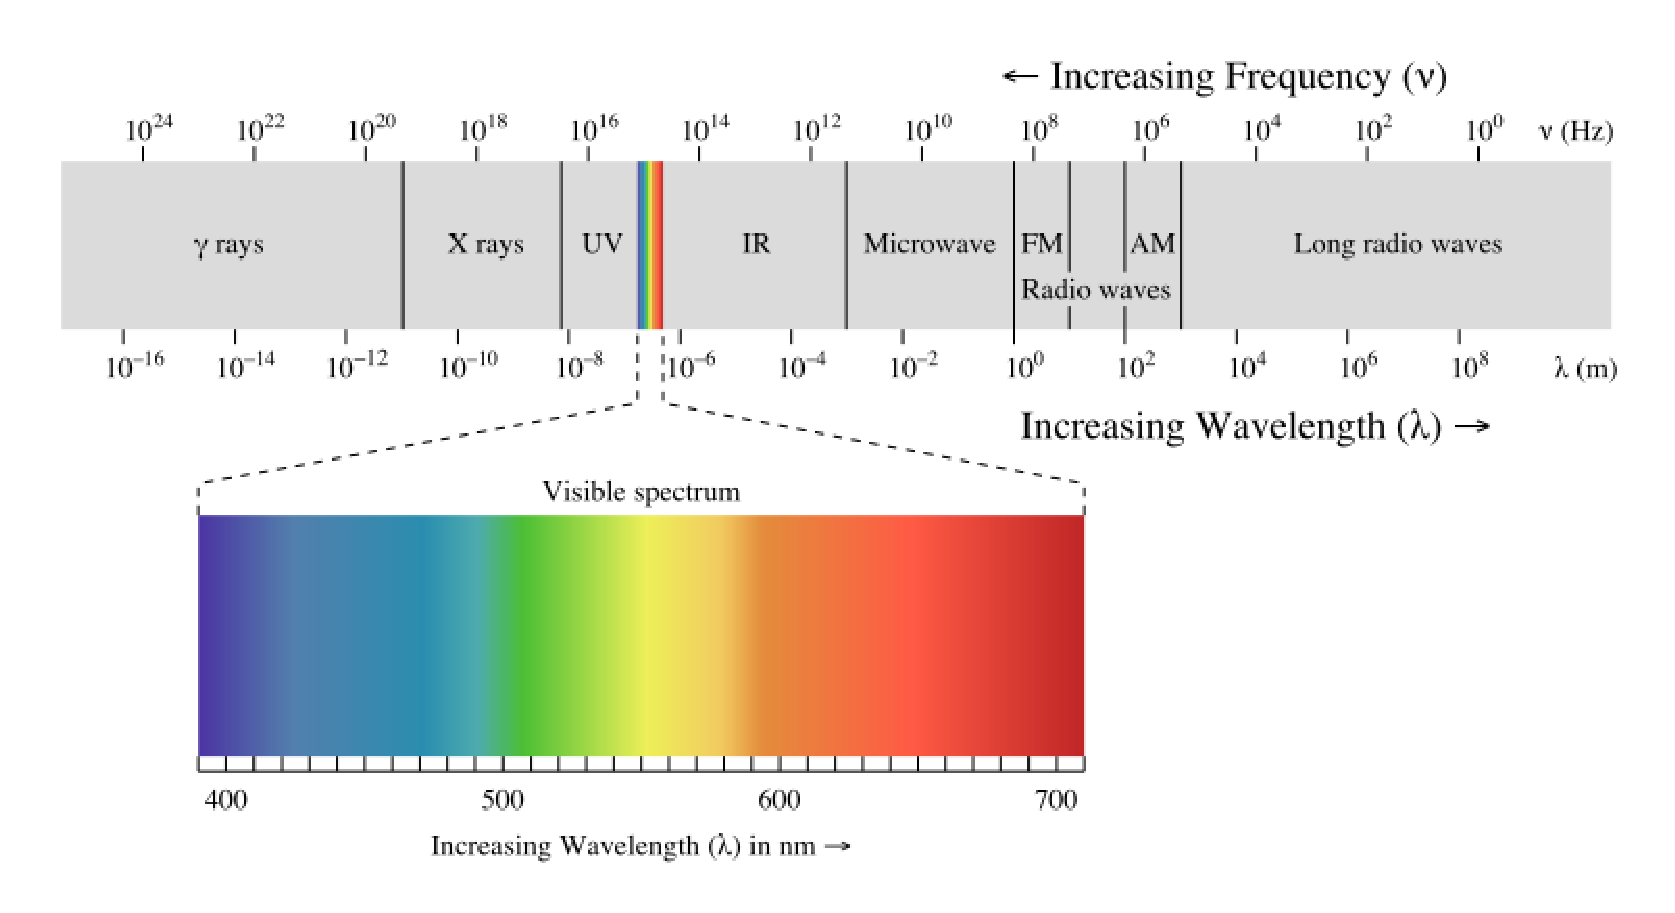
\includegraphics[width=13cm,angle=0]{images/cacharreria/espectro.eps}

{\small\bf Espectro Electromagn�tico (fuente Wikipedia)}
\end{figure}


\begin{multicols}{2}


Si seguimos bajando la frecuencia nos
encontramos las microondas y m�s abajo las frecuencias utilizadas por
la radio y la televisi�n. S� amigos, ten�is dispositivos de alta
frecuencia en vuestras cabezas XD.

Bien, la cuesti�n es que la regi�n del espectro (esto es, todas las
frecuencias posibles) que se considera radiaci�n infrarroja, est�
dividida en tres grandes grupos, que se llaman, respectivamente, IR-A,
IR-B e IR-C.

Con lo que nosotros vamos a jugar es con el IR-A, tambi�n conocido
como infrarrojo cercano... os imagin�is porqu� no?. Efectivamente, por
que es el que est� m�s cerca del espectro visible. S�, los m�s
interesantes son los otros, los que se usan para guiar misiles y para
obtener esas im�genes t�rmicas tan chulas que salen en las
pel�culas... pero efectivamente, hace falta algo m�s caro que una
webcam de 25 euros para jugar con esas cosas.

As� que ahora que tenemos una idea general de que es lo que estamos
haciendo... pues vamos a ponernos manos a la obra.


\sectiontext{white}{black}{DESMONTANDO LA C�MARA}

Nuestra webcam es una Logitech Messenger. Si, aprovechamos todo aqu�
en Occam's... Que!, �todav�a no os hab�is le�do el art�culo sobre video
vigilancia?... �a qu� est�is esperando?

Primer consejo, perded un poco de tiempo intentando descubrir que
ten�is que desmontar. Los tornillos suelen estar ocultos, porque son
antiest�ticos y, por la ley de Murphy, nosotros empezamos quitando
justo los que no necesit�bamos quitar XD.



Para poder desmontar esta webcam, tenemos que retirar una peque�a tapa
de goma que se encuentra en uno de los laterales de la esfera que
contiene la lente. En el agujero que cubre encontraremos un peque�o tornillo
que debemos retirar para poder acceder al interior de la c�mara.

\begin{center}
\myfig{0}{images/cacharreria/paso01.eps}{0.9}

{\footnotesize\bf Accediendo al tornillo.}
\end{center}


Por otra parte, con mucho cuidado, retiramos la carcasa gris azulada,
de la parte frontal, ayud�ndonos de un destornillador o cualquier cosa
que nos permita hacer palanca.

\begin{center}
\myfig{0}{images/cacharreria/paso02.eps}{0.9}

{\footnotesize\bf Quitando parte frontal.}
\end{center}


Ahora ya podemos acceder a la c�mara propiamente dicha, presionando el
clip que une las dos mitades de la esfera. 

\ebOpage{introcolor}{0.25}{LA CACHARRER�A}

Retiramos una de las
mitades, la gu�a de luz para poder ver el LED de actividad desde fuera
(un pedazo de pl�stico transparente), y ya tenemos nuestra c�mara 
``al desnudo'' :).

\begin{center}
\myfig{0}{images/cacharreria/paso03.eps}{0.9}

{\footnotesize\bf Ya casi estamos.}
\end{center}


El siguiente paso es desmontar la lente. En esta c�mara (y al parecer
en la mayor�a de las webcams), la lente se enrosca directamente sobre
el sensor que captura la imagen. As� que la giramos hasta que se
separe del circuito.

Ahora tenemos, por una parte, la placa de circuito impreso, con el
sensor de imagen y la rosca para la lente, y la lente por la otra.

\begin{center}
\myfig{0}{images/cacharreria/paso04.eps}{0.9}

{\footnotesize\bf Sensor de la webcam.}
\end{center}

\begin{center}
\myfig{0}{images/cacharreria/paso05.eps}{0.9}

{\footnotesize\bf La lente que acabamos de desenrroscar.}
\end{center}


\sectiontext{white}{black}{FILTRANDO LA LUZ}

Ooops!, no hab�amos dicho nada sobre esto. Bueno, lo decimos
ahora. Puesto que los sensores son sensibles al IR cercano, las
c�maras digitales traen incorporado un filtro IR, ya que de lo
contrario... bueno, eso lo podr�is comprobar vosotros mismos ;).

El objetivo de todo esto es sustituir ese filtro IR, por un filtro de
luz visible, de tal forma que la c�mara solo capte el IR cercano y no
la luz normal.

Como pod�is ver en la imagen, el filtro IR se encuentra (siempre para
nuestro modelo), en la parte de la lente, sujeto a ella con una
especie de pasta negra. Con un cutter eliminamos parte de esta pasta y
quitamos el filtro.

\begin{center}
\myfig{0}{images/cacharreria/paso06.eps}{0.9}

{\footnotesize\bf Filtro IR separado de la lente.}
\end{center}


Efectivamente, ese cristalito rosado es el filtro IR. Que os
esperabais, los filtros de luz son as�. Tiene que ser transparente,
para que pase la luz visible, y, pues eso, se llama infraRROJO por
algo :).


\begin{entradilla}
{\em El  {\color{introcolor}filtro IR} es un cristal rosado entre la
lente y el sensor.}
\end{entradilla}

La gran cuesti�n ahora es como hacer un filtro de luz visible. La
respuesta la sacamos de Internet, yo no ten�a ni idea la verdad,
lo �nico que ten�a claro, era que ten�a que ser algo oscuro.


Pues nuestro filtro lo haremos con un negativo fotogr�fico
velado... s�, �qui�n dir�a que alg�n d�a eso no ser�a tan f�cil de
conseguir eh?. Ojo, el negativo tiene que estar revelado y tendr�is
que escoger una de esas partes oscuras que normalmente quedan al
principio o final del rollo.

Para nuestro modelo de c�mara, utilizamos un perforador de hojas que
tiene aproximadamente el mismo di�metro que el orificio de la
lente. Acoplamos la lente de nuevo y a ver que pasa.

\ebOpage{introcolor}{0.25}{LA CACHARRER�A}

\begin{center}
\myfig{0}{images/cacharreria/paso07.eps}{0.9}

{\footnotesize\bf Nuestro filtro de luz visible.}
\end{center}


Nosotros probamos la c�mara antes de volver a montarla, pero vosotros
haced lo que quer�is :).

\sectiontext{white}{black}{A JUGAR}

Bien, pues despu�s de todo este l�o, vamos a ver que nos permite ver
nuestra nueva c�mara IR. En las p�ginas web de los recursos pod�is ver
varios ejemplos. Nosotros pondremos algunos m�s aqu�.

Lo primero que vamos a comprobar es que nuestro filtro de color
funciona. Para ello, simplemente vamos a capturar una imagen
multicolor y lo que esperar�amos obtener ser�a la misma imagen pero
sin colores... que no en blanco y negro. Como pod�is apreciar en la
imagen, hay una sutil diferencia.

\begin{center}
\myfig{0}{images/cacharreria/colores.eps}{0.9}
\end{center}


Parece funcionar bastante bien pero, normalmente, donde los filtros
suelen tener problemas es en las denominadas frecuencias de
corte. Para nuestro caso espec�fico, esa frecuencia de corte se
encuentra entre el rojo visible y el infrarrojo cercano. 

En la siguiente imagen utilizamos un puntero l�ser de esos de color
rojo para comprobar que lo que acabamos de decir tiene un cierto
sentido :P.

\begin{center}
\myfig{0}{images/cacharreria/puntero-laser.eps}{0.9}
\end{center}

Como pod�is ver en la imagen de la derecha, a�n cuando el color ha
sido eliminado de la escena, la luz roja proveniente del puntero l�ser
no es eliminada por nuestro filtro hecho con negativos fotogr�ficos
usados... bueno, nadie esperar�a que fuera perfecto.


Las pantallas TFT no se ven... pero la televisi�n es otra
historia. De la TV no tenemos im�genes, pero las pod�is obtener
vosotros mismos muy f�cilmente.

\begin{center}
\myfig{0}{images/cacharreria/monitor.eps}{0.95}
\end{center}


\sectiontext{white}{black}{VISI�N DE RAYOS X?}

Si busc�is m�s informaci�n sobre todo esto de las c�maras IR, os
encontrar�is entradas sobre ``milagrosos ingenios para mirar a trav�s de
las cosas''. S�, es que suenan as� de raros.

Lo que si es cierto es que al poder ``captuar'' la radiaci�n
infrarroja, y eliminar las componentes del espectro visible, ciertos
detalles de las im�genes se hacen m�s evidentes.

Por ejemplo, si miramos a este l�piz USB que utiliza una carcasa azul
transparente, apenas podemos ver su interior, pero si filtramos el
color (el azul en este caso), la superficie se vuelva pr�cticamente
transparente, y podemos ver los chips en su interior.

\begin{center}
\myfig{0}{images/cacharreria/usb.eps}{0.95}
\end{center}

Lo mismo sucede con estas gafas de sol. Para ser sincero, las gafas
que aparecen en la imagen son un poco cutres de estas de pl�stico, as�
que no podemos confirmar como funcionar�a con unas gafas de las buenas
:). Observad el ojo de Don... no nos la volver� a jugar en las
partidas de p�ker.

\begin{center}
\myfig{0}{images/cacharreria/gafas.eps}{0.95}
\end{center}

La raz�n de la popularidad de estas p�ginas es que supuestamente
permiten ver la ropa interior. Lamentablemente nadie se ha ofrecido
voluntario para ense�ar sus verg�enzas en aras de la ciencia.


\ebOpage{introcolor}{0.25}{LA CACHARRER�A}


\sectiontext{white}{black}{COSAS RARAS}

Como os adelant�bamos hace un momento, cuando eliminamos la radiaci�n
visible de nuestras im�genes, los distintos materiales de nuestras
ropas de muestran de diferentes formas.



En general, el color desaparece, ya que normalmente se consigue
utilizando un tinte que la �nica propiedad del material que modifica
es precisamente el color.

Aqu� pod�is ver como convertimos una moderno e informal chaqueta de
rayas, en un elegante traje blanco :).

\begin{center}
\myfig{0}{images/cacharreria/ropa.eps}{0.9}

\end{center}

Lo mismo sucede con las plantas que en general se ver�n de color
blanco, como pod�is observar en la siguiente imagen. Nuestro filtro de
color elimina el caracter�stico color verde.

\begin{center}
\myfig{0}{images/cacharreria/plantas.eps}{0.9}
\end{center}

Lo curioso de esto es que podemos hacer bonitas estampas invernales en
pleno agosto :).


Otra de las caracter�sticas de nuestra nueva c�mara es que nos permite
observar algunas de las medidas de seguridad incluidas en los
billetes. En la siguiente imagen pod�is observar un billete de 5 euros
y otros de 10.


\begin{center}
\myfig{0}{images/cacharreria/ejemplo01.eps}{0.9}
\end{center}

Como en la mayor�a de los ejemplos anteriores, gran parte del color
desaparece, pero la zona entorno al holograma, est� impresa con una
tinta especial (algo m�s que simplemente color). En el caso particular de los billetes, resulta m�s
efectivo e interesante utilizar luz ultravioleta o luz ``negra'' como
suele ser m�s conocida.

En la siguiente imagen podemos ver un billete de 50 y otro de 100 por
ambos lados. N�tese como el n�mero de serie y la cantidad se imprimen
con una tinta especial.

\begin{center}
\myfig{0}{images/cacharreria/billetes.eps}{0.9}
\end{center}


Finalmente, aqu� pod�is ver mi cartera que esta un poco para ser
retirada. Parece que las zonas mas desgastadas se resaltan en nuestra
camara IR. 

\begin{center}
\myfig{0}{images/cacharreria/cartera.eps}{0.9}

\end{center}




\sectiontext{white}{black}{LUZ INVISIBLE EN LA OSCURIDAD}

Y por supuesto, nuestro mando a distancia de la tele se convierte en
una linterna que no da luz XDDDDD. Y es precisamente esta
caracter�stica la que resulta m�s interesante desde el punto de vista
de las aplicaciones de nuestra webcam IR.

\begin{center}
\myfig{0}{images/cacharreria/linterna-ir.eps}{0.9}
\end{center}
\begin{center}
\myfig{0}{images/cacharreria/linterna-ir2.eps}{0.9}
\end{center}

Unas im�genes curiosas �eh?... Pero muchos os preguntar�is, y �para qu�
sirve esto?. Bueno, adem�s de para quedarte con los colegas. La
pregunta exacta que probablemente se os est� viniendo a la cabeza es:
�Qu� hace 
una gente tan discreta como los t�os de Occam's, con algo que solo sirve para
chulear?

Buena pregunta. Efectivamente, disponer de una c�mara IR nos permite
abordar algunos proyectos muy interesantes, sobre todo desde el punto
de vista de los denominado MMI ({\em Man Machine Interface} o Interface
Hombre M�quina).

La primera y la m�s obvia de estas aplicaciones es lo que los ingleses
denominan tracking y que nosotros podemos llamar seguimiento.

\ebOpage{introcolor}{0.25}{LA CACHARRER�A}

\sectiontext{white}{black}{TRACKING}

Como os dec�amos, las aplicaciones m�s interesantes y directas de este
tipo de c�maras es el de los interfaces MMI. La ventaja m�s
importante... pues que la radiaci�n infrarroja es invisible para el
ojo humano.

Esto se traduce en que nuestra c�mara va a capturar unas im�genes
totalmente oscuras con un pedazo de punto blanco all� donde haya una
fuente de luz infrarroja. Como pod�is imaginar, esto hace
pr�cticamente trivial el localizar esas fuentes de luz IR
en la imagen.

Para utilizar estas t�cnicas, tenemos dos opciones
fundamentales. Hacer que la ``cosa'' que queremos seguir emita luz IR,
o que la refleje.

En general si tenemos que seguir muchos puntos es mejor utilizar
elementos que reflejen la luz IR, de lo contrario habr�a que llenar el
objeto a seguir (pensad por ejemplo en un sistema de captura de
movimiento de personas para un juego) de cables y bater�as.



Si por el contrario, solo necesitamos un par de puntos de referencia,
por ejemplo para un dispositivo apuntador en un sistema de
realidad virtual, un par de LEDs y unas pilas har�n el trabajo.

\begin{entradilla}
{\em El {\color{introcolor} wiimote} utiliza una barra sensora con
{\color{introcolor} luz IR} para calcular la
posici�n del jugador}
\end{entradilla}

Este tipo de soluciones son utilizadas, por ejemplo, por el mando de la consola Wii (el
denominado wiimote), como parte de su sistema de
posicionamiento. El mando incluye un aceler�metro y una c�mara
infrarroja los cuales, junto con una barra sensora permiten calcular
la posici�n y orientaci�n del jugador.

\begin{center}
\myfig{0}{images/cacharreria/wiimote.eps}{0.7}
\end{center}


La barra sensora est� compuesta de dos grupos de LEDs infrarrojos,
separados una distancia conocida. La c�mara en el mando detecta estos
dos grupos y el procesador interno hace las matem�ticas :).

Con un pu�ado de LEDs infrarrojos, algunas resistencias y nuestra
webcam IR podemos explorar este tipo de sistemas.

\sectiontext{white}{black}{PANTALLAS T�CTILES}

Otra aplicaci�n en la que podemos utilizar nuestra flamante webcam IR
es la construcci�n de una pantalla t�ctil multi-toque :)... si, como
la Microsoft Surface y similares.


Este tipo de pantallas se pueden construir de distintas formas, pero
una de ellas, bastante asequible para el aficionado al cacharreo es la
denominada FTIR que son las siglas de {\em Frustrated Total Internal
Reflection}. Podr�amos traducirlo por Reflexi�n Interna Total
Frustrada, y enseguida veremos que el nombre tiene cierto sentido.

Estas pantallas utilizan una superficie acr�lica (un
pl�stico), en cuyo interior se inserta luz infrarroja, de forma que no
es visible por el ojo humano. La luz insertada rebota en el interior
del material pasando de un extremo al otro.

%\begin{center}
%\myfig{0}{images/cacharreria/multitouch.eps}{0.8}
%\end{center}


Si presionamos la superficie con, por ejemplo, nuestros dedos, la
deformaci�n que producimos en la superficie, interrumpe el rebote de
la luz IR en su interior y produce un efecto de dispersi�n... es
decir, que se produce un ``puntazo IR''... Ahora lo de reflexi�n
interna frustrada tiene m�s sentido �no?

Todo este proceso es completamente transparente al ojo humano ya que
la luz utilizada es IR. Pero para una c�mara IR, esos
``puntazos'' que se forman al presionar la superficie se pueden
capturar y procesar muy f�cilmente.

Otra t�cnica bastante utilizada en la denominada Iluminaci�n Difusa
({\em Diffuse Ilummination}). Existen dos formas de utilizar esta
t�cnica, pero la que nos interesa a nosotros es la denominada {\em
Rear Diffuse Illumination}. 

El sistema se basa en colocar un difusor
sobre la superficie t�ctil e iluminarlo con luz infrarroja. Cuan el
usuario pulsa sobre la superficie su dedo reflejara m�s luz IR que la
que refleja el difusor, de tal suerte que la c�mara pueda detectar el
punto correcto. El principal problema de esta t�cnica es el conseguir
una iluminaci�n uniforme en toda la superficie.

El hecho de que sea multi-toque o no, va a depender del software que
procese las im�genes y lo que ese software haga con los datos que obtenga.

Esto es todo. Esperamos que os haya gustado esta nueva secci�n. \EOP

\end{multicols}


{\colorbox{introcolor}{
\begin{minipage}{0.98\linewidth}
{\textsf
{\color{white}{\large RECURSOS}}

\medskip

\footnotesize
How to make a webcam work in infra red

{\footnotesize\url{http://www.hoagieshouse.com/IR/}}

%\medskip

Pantallas Multitouch FTIR

{\footnotesize\url{http://en.wikipedia.org/wiki/Total_internal_reflection\#Frustrated_total_internal_reflection}}

{\footnotesize\url{http://en.wikipedia.org/wiki/Multi-touch}}

NUI Group Community Book - ``Multi-Touch Technologies''

{\footnotesize\url{http://nuigroup.com/log/nuigroup_book_1/}}

%\medskip
\normalsize
}
\end{minipage}
}}


\clearpage
\pagebreak


% Este fichero es parte del N�mero 4 de la Revista Occam's Razor
% Revista Occam's Razor N�mero 4
%
% (c)  2009, The Occam's Razor Team
%
% Esta obra est� bajo una licencia Reconocimiento 3.0 Espa�a de
% Creative Commons. Para ver una copia de esta licencia, visite
% http://creativecommons.org/licenses/by/3.0/es/ o envie una carta a
% Creative Commons, 171 Second Street, Suite 300, San Francisco,
% California 94105, USA. 

% Seccion Tecnolog�a
%

\rput(8.5,-4.4){\resizebox{18.0cm}{!}{{\epsfbox{images/tecnologia/tecnologia.eps}}}}
%\rput(-2.5,-4.5){\resizebox{19cm}{!}{{\epsfbox{images/tecnologia/tecnologia.eps}}}}

% -------------------------------------------------
% Cabecera
\begin{flushright}
\msection{introcolor}{black}{0.25}{TECNOLOG�A}

\vspace{3.5cm}


%\mtitle{11cm}{{Reconocimiento Biom�trico a Trav�s de la Cara}}
\mtitle{8cm}{{Reconocimiento Biom�trico}}

\mtitle{6cm}{{a Trav�s de la Cara}}

{\sf por Fernando Mart�n Rodr�guez (fmartin@tsc.uvigo.es) }

{\psset{linecolor=black,linestyle=dotted}\psline(-12,0)}
\end{flushright}

\vspace{2mm}

% -------------------------------------------------

\begin{multicols}{2}

% Introducci�n
\intro{introcolor}{S}{iendo �ste un n�mero dedicado a las tecnolog�as
de seguridad no pod�a faltar un art�culo de la serie
biom�trica. Advertido queda que seguramente ser� el �ltimo... Ante lo
que seguramente estar� pensando la direcci�n de la revista digo que
no, no me siento capaz de escribir sobre el reconocimiento a trav�s de
voz. Hoy toca el reconocimiento a trav�s de im�genes de la
cara. 
}

\vspace{2mm}

% Cuerpo del art�culo
Fijaos que ese el m�todo que m�s empleamos los humanos para
reconocer personas. En el 99\% de los casos reconocemos a alguien al
ver su cara, tambi�n reconocemos personas por la voz pero casi siempre
vemos las caras antes de o�r nada. Ya puestos, comentar que el
reconocimiento humano es muy fiable porque utiliza m�ltiples datos,
esto es: vemos la cara pero tambi�n la silueta (la estatura,
complexi�n...), o�mos la voz y tambi�n nos fijamos en cosas muy
dif�ciles de medir para una m�quina: los gestos, la forma de
andar.... La suma de todos esos factores (una suma ponderada que hace
el cerebro sin que lo notemos) da un reconocimiento muy
fiable. Realmente ese m�todo (la redundancia) es el que usa el cerebro
humano para casi todas sus tareas de reconocimiento. 


\sectiontext{white}{black}{INTRODUCCI�N}

Para mantener la tradici�n, empezaremos recordando las caracter�sticas
que un rasgo debe cumplir para dar lugar a un buen sistema biom�trico
y, ya de paso, veremos c�mo se cumplen para las im�genes faciales. A
saber: 

\begin{itemize}
\item Universalidad: todas las personas deben poseer el rasgo. Bueno,
eso es cierto... por lo menos para personas vivas. 

\item Unicidad: no debe haber dos personas con el rasgo seleccionado
igual. Aqu� ya empezamos a no cumplir... aparte de gemelos id�nticos
tambi�n hay pares de personas parecidas (m�s probables en gente con
parentesco pero no necesariamente).

\item Permanencia: debe ser invariantes con el tiempo. ��La cagamos!!
No hay rasgo biom�trico m�s variable que la cara: barba, gafas, pelo
largo o corto... Aparte de las diferencias (notables) que puede llegar
a haber en la captura de imagen debidas a la postura frente a la
c�mara (pose), el gesto (sonrisa, enfado, bostezo ...). Pensad que en
caso de usuarios malintencionados podremos tener casos de
disfraz. Todo lo anterior, unido a que el n�mero de im�genes que
podemos tener almacenadas de la cara de alguien es limitado hace que
�ste sea uno de los rasgos biom�tricos menos fiables que se conocen. 

\item Cuantificaci�n: admiten medidas cuantitativas. S� que las
admiten... si no, no ser�a posible ni intentarlo y no estar�amos
escribiendo esto. 

\end{itemize}



\begin{entradilla}
{\em El {\color{introcolor} reconocimiento de caras es el m�todo} m�s utilizado por los
humanos para reconocer personas}
\end{entradilla}

Aun a riesgo de repetirme, voy a copiar otra vez el cuadro comparativo
de los diferentes sistemas biom�tricos. Recordad que TFA significa
``Tasa de Falsa Aceptaci�n'' y es el porcentaje de veces que el
sistema declara como iguales a dos individuos que no lo son, mientras
que TFR es ``Tasa de Falso Rechazo'' y es el porcentaje de veces que
dos individuos iguales son err�neamente considerados
diferentes. Fijaos que aunque dichas tasas pueden llegar a ser bajas
(en experimentos muy controlados), la memoria y el tiempo requeridos
son altos y la facilidad de enga�ar al sistema tambi�n. 





\eOpage

\msection{introcolor}{black}{0.25}{TECNOLOG�A}


\begin{table}[ht]
{\footnotesize
\begin{tabular}{|p{1.6cm}|p{0.8cm}|p{0.8cm}|p{1.5cm}|p{1.7cm}|p{1.7cm}|p{1.7cm}|p{1.7cm}|p{1.7cm}|}
\hline
{Indicador biom�trico} & {TFR} & {TFA}
& {Memoria (bytes)} & {Tiempo respuesta} 
& {Variabilidad intra-clase} & {Variabilidad
inter-clase} & {Implantaci�n en mercado} & {Facilidad  de enga�o}\\
\hline
%\rowcolor{gray}
Huellas & 3\% & $1 : 1 ^6$ & 100-1000 & Depende del sistema & Media & Alta &52\% & Media \\
\hline
Retina & Bajas & aprox. 0\% & Poca & Bastante bajo & Muy baja & Muy alta & <1\% & Baja \\
\hline
%\rowcolor{gray}
Iris & Bajas & aprox. 0\%  & 1024 bits & Medio-bajo & Muy baja & Muy alta & 7,3\% & Baja \\
\hline
Cara & Bajas & Bajas & >10,000  & Alto(1:N)  Bajo (1:1) & Muy alta & Alta & 11,4\% & Muy alta\\
\hline
%\rowcolor{gray}
Voz & Bajas & Bajas & >1000 & Alto (1:N)  Bajo (1:1) & Alta & Media-alta & 4,1\% & Muy alta \\
\hline


\end{tabular}
}
\end{table}
\begin{center}
{\textbf {Tabla 1: Principales caracter�sticas de algunos indicadores biom�tricos.}}
\end{center}

\begin{multicols}{2}




El conocido gur� de la seguridad Bruce Schneier (inventor del
algoritmo de cifrado Blowfish) escribi� que era inviable el uso de un
sistema de reconocimiento de caras en una aplicaci�n masiva como, por
ejemplo, detectar sospechosos en un aeropuerto. Con una TFA t�pica del
1\% significar�a ``parar'' a una de cada 100 personas que pasen por
delante de una c�mara (y obligarles a identificarse utilizando un
m�todo m�s fiable, por ejemplo: colocando el �ndice en un lector
autom�tico de huellas). Si en Barajas hay casi 150000 pasajeros al d�a
(ese es el dato que encontr� en Internet) tendr�amos que identificar a
1500 personas/d�a. ���Ojo!!! que no estamos contando a los que van a
esperar a alguien... Adem�s, ser identificado por la polic�a para que
resulte ser un error es algo bastante desagradable y que puede dar
lugar a denuncias, quejas... �Qu� ocurrir�a en el aeropuerto de
Chicago (m�s de 250.000 pasajeros/d�a)? 

El reconocimiento de caras s� es viable en grupos cerrados de pocos
usuarios (control de acceso a un recinto o a un sistema
inform�tico...) y es en esos casos cuando se obtienen buenos
resultados en TFR y TFA. 


\sectiontext{white}{black}{PREPROCESADO}

Como en todo problema de reconocimiento de im�genes, primero debemos
extraer la zona de inter�s. En el reconocimiento de caras se suele
buscar una cara frente a la c�mara, con los ojos en posici�n conocida
y de un tama�o fijo. Adem�s, deber�amos normalizar el brillo de la
imagen de forma que no haya variaciones grandes de iluminaci�n. Llegar
a tener esa imagen a partir de lo que ha capturado la c�mara es lo que
llamamos preprocesado y es muy importante hacerlo bien para que el
reconocimiento funcione. En im�genes capturadas ``de cualquier manera'',
esto es: las im�genes de una c�mara de seguridad que apunta a un
pasillo o a una cola de personas puede no ser posible hacer un
preprocesado correcto. 

\begin{entradilla}
{\em Comenzaremos {\color{introcolor} preprocesando} las las im�genes}
\end{entradilla}

A continuaci�n describiremos dos t�cnicas muy populares para localizar
caras. Adem�s, no son excluyentes, pudiendo haber sistemas que
combinen ambas. 

\sectiontext{white}{black}{LOCALIZACI�N POR COLOR}

Una de las t�cnicas m�s empleadas para localizar caras es la detecci�n
de aquellos puntos de la imagen que tienen un color similar al de la
piel humana. Este m�todo nos dar� una serie de regiones con alta
probabilidad de contener caras. Cada una de esas regiones (blobs)
deber� ser procesada posteriormente para determinar si realmente es
una cara o no. Una aplicaci�n es, por ejemplo, buscar caras en una
imagen compleja e impredecible (como las im�genes de una c�mara de
vigilancia). 

Para entender bien la localizaci�n por color debemos saber que la
representaci�n habitual de los colores (R, G, B) no es la �nica
posible y se puede transformar a otras representaciones (espacios de
color), todas ellas basadas en tres componentes. Una representaci�n
muy interesante es la HSV que divide el color en tres n�meros: 

\begin{itemize}
\item El tinte (Hue, H): es un �ngulo y define la posici�n del color en un
c�rculo que empieza en el rojo (�ngulo 0) y que recorre todo el arco
iris. El tinte es lo que coloquialmente llamamos ``color'': rojo,
naranja, verde \ldots Otra cosa es que rojo sea intenso, brillante \ldots

\item La saturaci�n (Saturation, S): se mide entre 0 y 1 y es la
``pureza'' del color. Si compramos pintura roja deber�a ser rojo puro
(saturaci�n 1 o rojo al 100\%). Si deseamos ``rebajar'' ese rojo,
podemos mezclar la pintura roja con blanca e iremos logrando
diferentes ``niveles'' de rojo, si tenemos 50\% de rojo y 50\% de
blanco la saturaci�n ser� 0.5.

\item El brillo (llamado Value, V; a veces se le llama intensidad y se
habla de sistema HIS): el brillo es la ``potencia'' del color o la
iluminaci�n que proporciona. El color blanco es el m�s brillante y el
negro tiene brillo cero. Hace a�os se usaban monitores verdes porque
es un color que da gran sensaci�n de brillo para poco gasto en
energ�a, las luces azules para estudiar usan la idea contraria (es un
color que ilumina poco pero cansa menos la vista).  

\end{itemize}

\ebOpage{introcolor}{0.25}{TECNOLOG�A}


\begin{center}
\myfig{0}{images/tecnologia/circulo_color.eps}{0.9}

{\footnotesize\bf C�rculo de Color. El �ngulo polar determina el
tinte, la distancia al centro la saturaci�n.}
\end{center}

Para la piel humana\ldots.
\begin{itemize}

\item El tinte es ���naranja!!! �Qu� ocurre si subimos mucho el color del
televisor? No nos vemos naranjas porque la saturaci�n es baja. 

\item El color var�a mucho para los diferentes tipos de piel. La raza
amarilla es la m�s ``saturada''. La raza negra tiene brillo muy bajo
(y eso puede introducir errores de redondeo en el c�lculo del tinte).

\item Para hacer un reconocedor serio debemos utilizar reconocimiento
de patrones. Esto es: tomar muchas fotos de individuos con diferentes
tipos de piel y, de alguna manera, comparar la imagen que tengamos a
la entrada con las previas (conjunto de entrenamiento).

\item El sistema de color HSV es el m�s intuitivo para este problema pero se utilizan otros. 

\end{itemize}

Para ampliar un poco estos conocimientos pod�is leer el sencillo art�culo: ``Detecci�n de Caras en Im�genes Capturadas por C�maras Web'' (autores: Patricia Conde Pardo y yo mismo). S�, s�, lo he vuelto a hacer: ``me acabo de hacer autobombo''. Lo pod�is descargar de {\footnotesize{\url{http://webs.uvigo.es/gpi-rv/research-papers.html}}}.


\sectiontext{white}{black}{EL ALGORITMO DE VIOLA}

Actualmente existe un m�todo capaz de detectar caras de cualquier
tama�o en una imagen blanco y negro. Fue dise�ado por Paul Viola y
publicado en ``Rapid Object Detection using a Boosted Cascade of
Simple Features,'' (autores P. Viola y M. J. Jones, publicado en 2001
en el congreso del IEEE sobre visi�n artificial y reconocimiento de
patrones: CVPR). Para este algoritmo disponemos de una implementaci�n
de c�digo abierto (ver cuadro de recursos).

Este c�digo es parte de la excelente biblioteca ``OpenCV'' (conjunto
de algoritmos de visi�n artificial donados por Intel al mundo):
{\footnotesize\url{http://www.intel.com/technology/computing/opencv}}. Ufff,
las multinacionales, a veces, tambi�n tienen su corazoncito :).

\begin{entradilla}
{\em El {\color{introcolor}algoritmo de Viola} se basa en la extracci�n de
caracter�sticas de tipo Haar}
\end{entradilla}

El algoritmo se basa en las llamadas ``Haar-like features''
(caracter�sticas tipo Haar, que se llaman as� porque se calculan de
una forma parecida a una transformada llamada ``transformada Haar'' o
wavelet de Haar). Cada caracter�stica es como un operador gradiente
pensado para resaltar un patr�n. Los patrones son caracter�sticas
como: contornos, l�neas, cruces\ldots La imagen se recorre con una
ventana a la que se le aplican varios clasificadores en serie, cada
uno m�s complejo que el anterior, que usan las caracter�sticas para
confirmar o descartar la hip�tesis de que estamos ante el objeto
buscado (en este caso una cara pero podr�a entrenarse para encontrar
otros objetos). Si la hip�tesis se rechaza en cualquier nivel, el
proceso no contin�a pero si se confirma tras todos los filtros
tendremos un objeto detectado. 


\end{multicols}

\begin{figure}[ht]
\centering
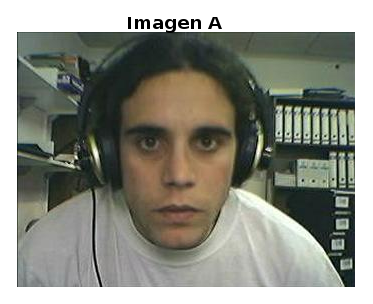
\includegraphics[height=4.0cm,angle=0]{images/tecnologia/imagenA.eps}

\includegraphics[height=4.0cm,angle=0]{images/tecnologia/imagenB.eps}
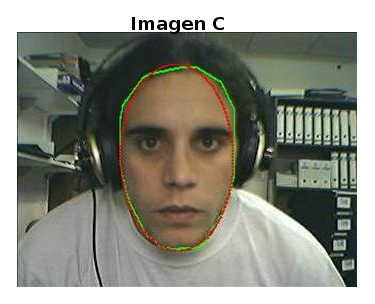
\includegraphics[height=4.0cm,angle=0]{images/tecnologia/imagenC.eps}

{\footnotesize\bf A: Imagen original. B: se ha aumentado la saturaci�n logrando resaltar la piel visualmente (y hacer evidente el tinte anaranjado). C: detecci�n del �valo facial utilizando colorimetr�a (se ha obtenido un blob del que se ha calculado un contorno poligonal: en verde, y una elipse de ajuste: en rojo).
}
\end{figure}

\clearpage
\pagebreak

\msection{introcolor}{black}{0.25}{TECNOLOG�A}

\begin{figure}[ht]
\centering
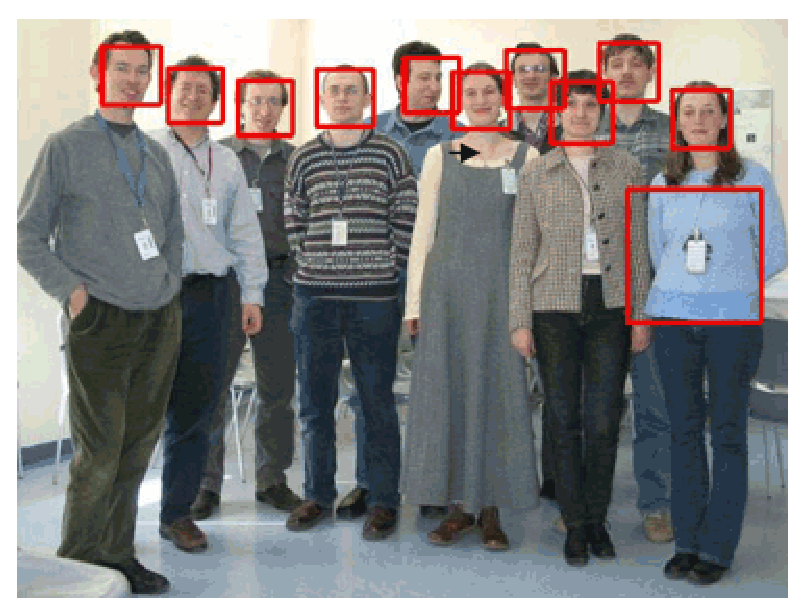
\includegraphics[height=9.0cm,angle=0]{images/tecnologia/resultado.eps}

{\footnotesize\bf Resultado de aplicar la funci�n OpenCV. N�tese que
hay un falso positivo.}
\end{figure}

\bigskip

\begin{multicols}{2}



Los patrones se consideran girados en varios posibles �ngulos. Adem�s,
el algoritmo puede ejecutarse a varias escalas para obtener objetos de
diferentes tama�os o de tama�o desconocido. 

Una vez que hemos localizado las caras en nuestra imagen, ha llegado
el momento de reconocerlas. Se han probado muchas t�cnicas para el reconocimiento facial. Aqu� s�lo vamos a describir las dos m�s extendidas.


\sectiontext{white}{black}{AN�LISIS DE COMPONENTES PRINCIPALES}

El an�lisis de componentes principales (o PCA: Principal Component
Analysis) se basa en representar las caras como combinaci�n lineal de
ciertas caras b�sicas (autocaras).Adem�s, conocemos cu�les son las
autocaras m�s importantes por lo que podemos quedarnos s�lo con ellas
y descartar las dem�s. Los coeficientes que permiten representar la
cara de entrada ser�n utilizados como caracter�sticas para el
reconocimiento. A esta t�cnica tambi�n se le llama proyecci�n en
subespacios o tambi�n ``transformada de Karhunen-Lo�ve''.

\begin{entradilla}
{\em El proceso de reconocimiento hace uso de {\color{introcolor}�lgebra matricial}}
\end{entradilla}

El nombre de proyecci�n en subespacios viene de la teor�a matem�tica
que se utiliza: se trata de convertir el conjunto de im�genes de caras
en un subespacio vectorial (un subconjunto de un espacio mayor: el de
im�genes). Para realizar el an�lisis debemos encontrar una base del
subespacio, esto es: un conjunto de caras tal que podamos representar
cualquier cara como combinaci�n lineal de las caras de la base. Es
m�s: no nos vale cualquier base... queremos una base ``ordenada en
importancia''. 

\begin{entradilla}
{\em El PCA nos permite {\color{introcolor} generar una base de vectores} ordenada por importancia}
\end{entradilla}

Quiero decir: el primer vector ser� el m�s importante, el segundo ya ser� menos importante pero m�s que los siguientes... Una base con esas caracter�sticas ``concentra la informaci�n en los coeficientes de los primeros vectores''. Podremos llegar a decidir que, por ejemplo, los 50 primeros componentes son suficientes con lo que los otros (N-50, con N muy grande) los ignoramos. Si al representar una imagen con los 50 primeros coeficientes obtenemos una distancia eucl�dea baja respecto de la imagen original: ``Esa imagen ser� una cara''. Si la distancia obtenida es grande, no ser� una cara; ser� otra cosa.


�C�mo se consigue lo anterior? Bueno\ldots en cuatro palabras: ``utilizando �lgebra de matrices'' (no me atrevo a decir que es �lgebra avanzada pero puede desafiar un poco los conocimientos olvidados del ingeniero medio). Suponiendo que nuestras caras son im�genes $MxM$, tendremos un espacio total de dimensi�n $N=M^2$. Tomando muchas caras podemos calcular una matriz de autocorrelaci�n para esos vectores (que resumir� la ``estad�stica'' de las caras). Ahora empieza lo ``fuerte'':


\ebOpage{introcolor}{0.25}{TECNOLOG�A}

\begin{itemize}
\item La matriz de autocorrelaci�n ser� definida positiva (esto es:
todos sus autovalores son reales y positivos) �lgebra) por lo que
podremos construir una base ortonormal de autovectores (cre�roslo, es
un teorema). �Qu� es una base ortonormal? Aqu�lla formada por vectores
unitarios y perpendiculares entre s�. 

\item Esa ser� nuestra base. Los autovectores se les llama
``autocaras'' porque son eso: caras (que pueden combinarse para formar
cualquier cara). La autocara m�s importante es la asociada al mayor
autovalor y as� sucesivamente (ordenando los autovalores de mayor a
menor tenemos ordenada la base).

\item Una vez hecho esto habr�a que decidir cu�ntos vectores retenemos
y cu�ntos descartamos... un indicativo puede ser el peso de los
autovalores. Una medida simple como:  $\rho =
{(\displaystyle\sum_{i=1}^p \lambda_i)} /
{(\displaystyle\sum_{i=1}^N \lambda_i)}$estima el peso de los p
primeros autovalores respecto del total: si  $\rho$ es cercano a 1 el peso es grande. De todas formas, el n�mero suficiente de componentes debe ser verificado experimentalmente. Esto es: si implement�is esto y no funciona tal vez haya que subir p. Otro m�todo es empezar con p muy grande e irlo bajando hasta que falle (funcionar/fallar significa que el conjunto de p autocaras representa bien las caras (peque�o error eucl�deo).


\end{itemize}

Pensad que con todo esto hemos reducido la dimensi�n del espacio de caras de $N=M^2$ a p. Si $M=512$ y $p=50$

Cuando queremos reconocer una imagen lo primero es calcular sus coeficientes para las autocaras seleccionadas. A eso se le llama ``proyectar sobre el subespacio de autocaras'' (de hecho, el coeficiente para cada autocara es muy f�cil de calcular, basta un producto escalar entre la autocara y la cara de entrada).

Despu�s podr�amos comprobar si la entrada es realmente una cara
(calculando el error entre la cara representada por las autocaras y la
cara misma). Si esa comprobaci�n es positiva (error bajo), ahora toca
saber de qui�n es la cara... para eso, hay que comparar el vector de
caracter�sticas de la cara de entrada (coeficientes de la cara
respecto a las autocaras) con los vectores almacenados (procedentes de
caras que queremos reconocer). 


\end{multicols}


{\colorbox{excolor}{
\begin{minipage}{0.98\linewidth}

{\Large PCA f�cil}

Para intentar hacer m�s comprensible esto de los subespacios, permitidme un ejemplo muy simplificado. Supongamos que nuestras im�genes son de tama�o 2x1 (eso s� que es simplificar). Entonces las im�genes ser�n puntos del plano (figura de la izquierda).


\begin{centering}
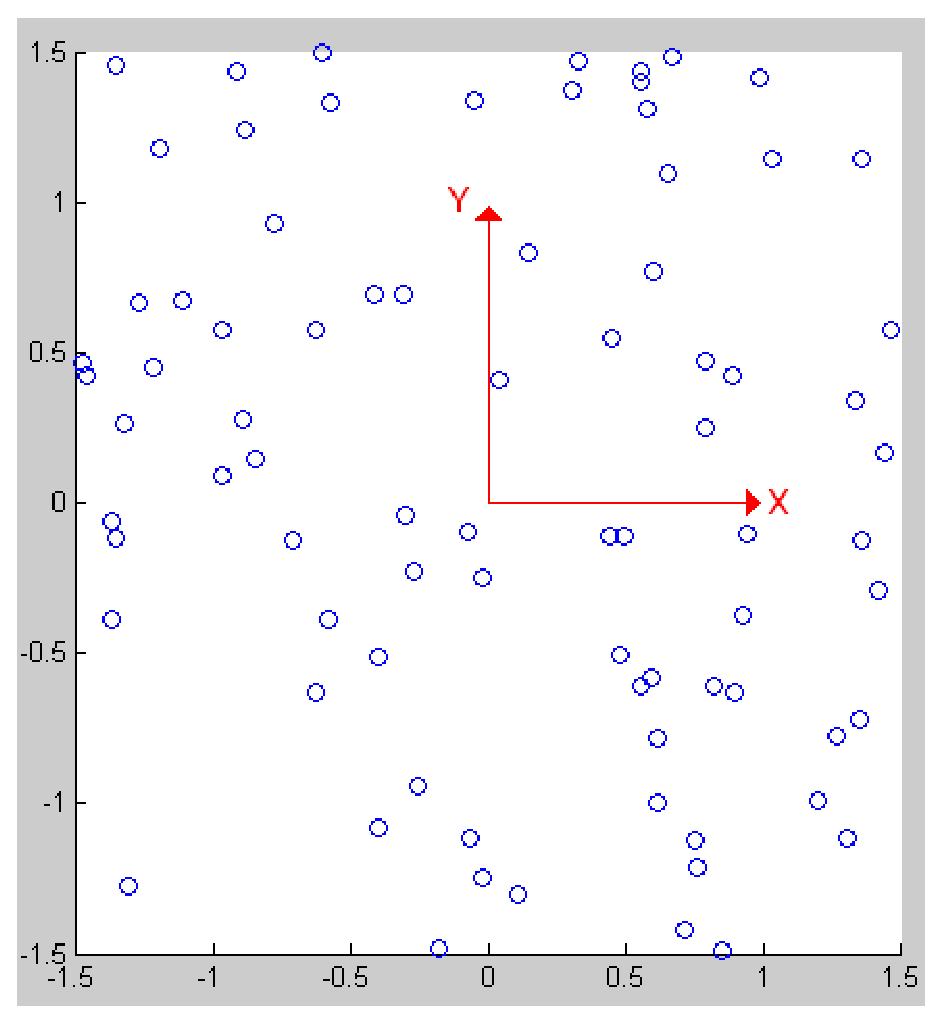
\includegraphics[height=8.5cm,angle=0]{images/tecnologia/vectores.eps}
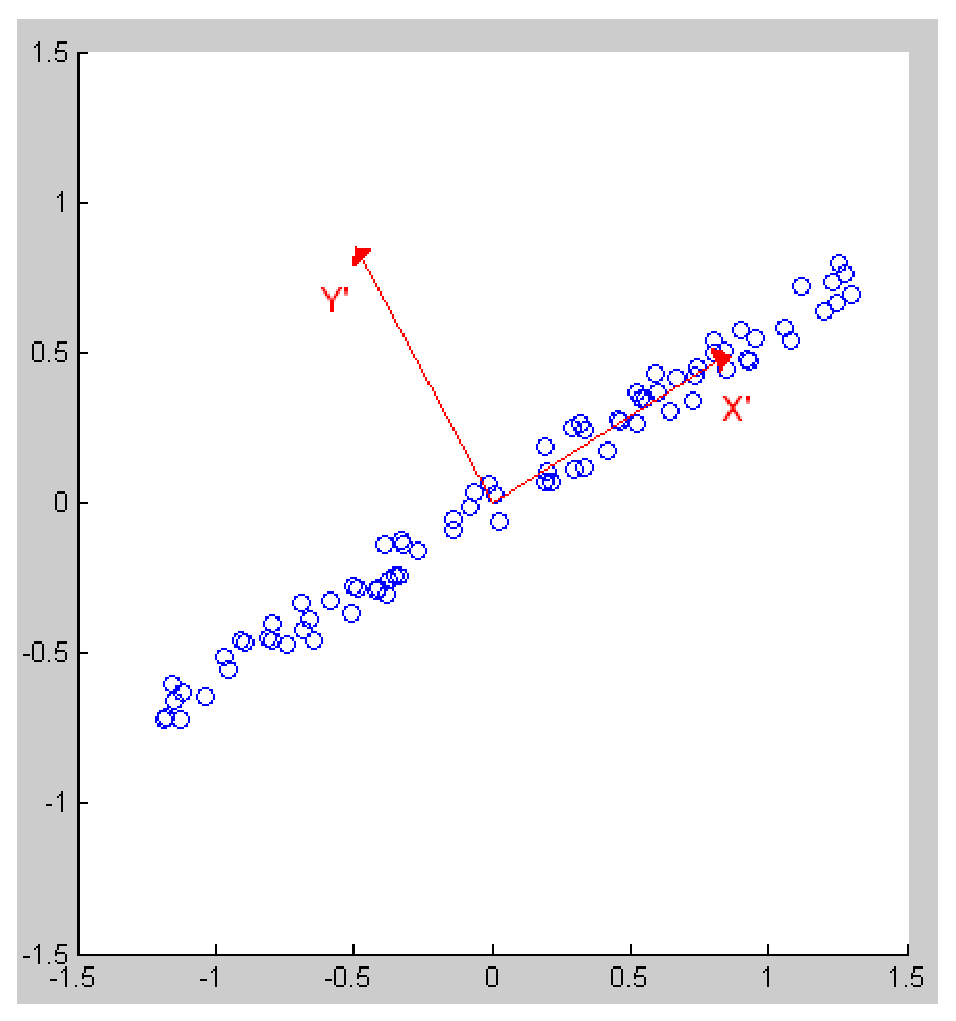
\includegraphics[height=8.5cm,angle=0]{images/tecnologia/vectores_transformados.eps}
\end{centering}

El ``quiz'' de la cuesti�n es que no nos interesan todas las im�genes,
s�lo queremos procesar caras. Siguiendo con nuestra simplificaci�n, si
las im�genes de inter�s son puntos que ``aproximadamente'' est�n
situados sobre la misma recta (figura de la derecha); podremos hacer
una simplificaci�n (creaci�n de una base de autovectores) que viene a
ser un giro de ejes de forma que la primera componente quede en la
direcci�n principal. 

�Podemos despreciar la componente $Y'$? Yo dir�a que s�. Adem�s,
podemos saber f�cilmente si un vector es del conjunto: si la
representaci�n eliminando $Y'$ comete un error peque�o �NO? 

\bigskip

\end{minipage}
}}


\clearpage
\pagebreak

\msection{introcolor}{black}{0.25}{TECNOLOG�A}

\begin{figure}[ht]
\centering
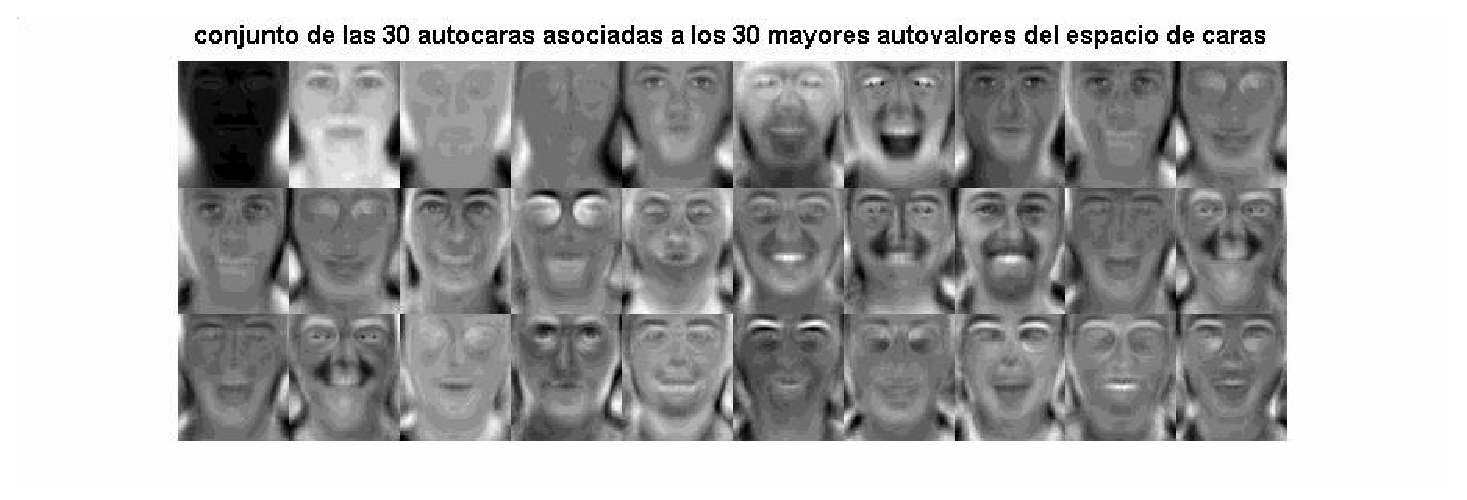
\includegraphics[height=4.5cm,angle=0]{images/tecnologia/autocaras.eps}

\includegraphics[height=2.0cm,angle=0]{images/tecnologia/cara-media.eps}

{\footnotesize\bf Ejemplo de un conjunto de autocaras. La
autocorrelaci�n se hace restando la media a cada muestra por lo que
debemos tenerla tambi�n.}
\end{figure}

\bigskip

\begin{multicols}{2}


Aqu� se pueden usar muchas t�cnicas pero la m�s simple (y una de las
m�s efectivas) es la del vecino m�s pr�ximo. Esta t�cnica consiste en
calcular distancias entre los vectores de caracter�sticas (eucl�dea o
norma 2, norma 1...) y considerar como resultado reconocido, el patr�n
almacenado m�s pr�ximo al de entrada. ���Ojo!!! puede haber varias
muestras por individuo a reconocer. 

\begin{center}
\myfig{0}{images/tecnologia/proyeccion.eps}{0.9}

{\footnotesize\bf Proyecci�n en subespacio de caras.}
\end{center}


\sectiontext{white}{black}{T�CNICAS DE REPRESENTACI�N CON MALLAS
DEFORMABLES}

La idea de este m�todo es ``colocar una m�scara deformable sobre la cara (con forma de red o malla) y ajustarla para que los nodos de la malla coincidan con puntos importantes como los ojos, nariz\ldots (puntos fiduciales)''. Este m�todo es la versi�n inform�tica del m�todo que hemos visto muchos en televisi�n: encontrar caracter�sticas como la distancia entre los ojos, la posici�n de la punta de la nariz\ldots



La base matem�tica del m�todo es aplicar filtros de Gabor en cada nodo y utilizar las respuestas obtenidas para ir ajustando la malla hasta que est� colocada sobre los puntos deseados. Como vimos en el cap�tulo de las huellas el filtro de Gabor extrae caracter�sticas del entorno del punto, adem�s los filtros Gabor tienen una orientaci�n que hace que sean sensibles a las variaciones con determinado �ngulo. Aplicando los filtros en m�ltiples direcciones podemos calcular una especie de vector gradiente que nos permita mover el nodo en la direcci�n deseada.


\begin{entradilla}
{\em la localizaci�n de los {\color{introcolor}puntos fiduciales de la cara} es m�s
compleja de lo que parece en la TV}
\end{entradilla}

Una vez ajustadas las mallas, los sujetos se comparan mediante una medida de similitud que tiene dos t�rminos: la similitud entre los vectores de textura de cada nodo y la similitud por deformaci�n de cada malla.

\begin{center}
\myfig{0}{images/tecnologia/malla.eps}{0.4}

{\footnotesize\bf Representaci�n con mallas deformables (m�todo EBGM:
Elastic Bunch Graph Matching.}
\end{center}

\sectiontext{white}{black}{TRABAJOS DE LA ETSET VIGO}

En nuestro centro, el profesor Jos� Luis Alba (jalba@gts.tsc.uvigo.es)
y varios colaboradores llevan alg�n tiempo trabajando en el
reconocimiento a trav�s de caras. Dichos trabajos forman parte de una
l�nea m�s amplia dedicada al reconocimiento biom�trico en
general. 


\ebOpage{introcolor}{0.25}{TECNOLOG�A}



Originalmente s�lo se trabaj� con reconocimiento por voz
(reconocimiento de locutores) y posteriormente se a�adieron los
reconocimientos de caras, iris y huellas. Actualmente, se est�
desarrollando un sistema de verificaci�n multimodal (voz y cara) para
acceso a servicios a trav�s de Internet. Esta l�nea de investigaci�n
se sigue en cooperaci�n con otros grupos de trabajo europeos en el
seno de la acci�n COST275: ``Biometrics-Based Recognition of people
over the Internet'' (\url{http://www.fub.it/cost275}). Como parte de las
actividades del COST se organiz� un workshop (peque�o congreso) en el
que se presentaron los �ltimos avances en el campo
(\url{http://cost275.gts.tsc.uvigo.es/}). Adem�s, estos estudios del reciben
financiaci�n a trav�s de proyectos del Ministerio de Educaci�n y de la
Xunta de Galicia y parten de un sistema ya desarrollado previamente
con fondos p�blicos en el que se utilizaba reconocimiento de voz para
acceder a un buz�n de correo por l�nea telef�nica
(\url{http://www.gts.tsc.uvigo.es/telcorreo/}).  \EOP

\end{multicols}

\rput(8,-15.0){\resizebox{!}{16cm}{{\epsfbox{images/general/promo-1.eps}}}}

{\colorbox{introcolor}{
\begin{minipage}{0.98\linewidth}
{\textsf
{\color{white}{\LARGE RECURSOS}}

\bigskip

\textsf{Implementaci�n de C�digo Abierto del algoritmo de Viola}

{\footnotesize\url{http://www.intel.com/technology/itj/2005/volume09issue02/art03_learning_vision/p04_face_detection.htm}}

\medskip

\textsf{Librer�a OpenCV}

{\footnotesize\url{http://www.intel.com/technology/computing/opencv}}

\medskip

\textsf{Recursos en ETSET Vigo}

{\footnotesize\url{http://www.fub.it/cost275}}

{\footnotesize\url{http://cost275.gts.tsc.uvigo.es/}}

{\footnotesize\url{http://www.gts.tsc.uvigo.es/telcorreo/}}

}
\end{minipage}
}}





\clearpage
\pagebreak

% Este fichero es parte del N�mero 4 de la Revista Occam's Razor
% Revista Occam's Razor N�mero 4
%
% (c)  2009, The Occam's Razor Team
%
% Esta obra est� bajo una licencia Reconocimiento 3.0 Espa�a de
% Creative Commons. Para ver una copia de esta licencia, visite
% http://creativecommons.org/licenses/by/3.0/es/ o envie una carta a
% Creative Commons, 171 Second Street, Suite 300, San Francisco,
% California 94105, USA. 

% Secci�n Trucos


\rput(3,-2.5){\resizebox{!}{6cm}{{\epsfbox{images/general/varita3.eps}}}}
\begin{flushright}
\msection{red}{black}{0.1}{TRUCOS}

\mtitle{6cm}{Con un par... de l�neas}

\msubtitle{8cm}{Chuletillas para hacer cosas m� r�pido}

{\sf por Tamariz el de la Perd�z}

{\psset{linecolor=black,linestyle=dotted}\psline(-10,0)}

\end{flushright}

\vspace{4mm}

\begin{multicols}{2}
\raggedcolumns


\sectiontext{white}{black}{GDB CON INTERFAZ MAS AMIGABLE}
\hrule
\vspace{2mm}

El depurador de GNU gdb, proporciona un interfaz {\em m�s amigable},
si es que eso es posible. Para echarle un ojo, solo ten�is que utilizar la
opci�n {\tt -tui} (algo as� como {\em Text User Interface}). Lo que obtendr�is es algo como esto:

\myfig{0}{images/trucos/gdb_tui.eps}{0.8}
\vspace{2mm}

Os adelantamos que, este interfaz se suele ir a paseo en cuanto
nuestro programa empieza a escribir cosas en la consola. Si necesit�is algo todav�a m�s amigable pod�is probar {\tt cgdb}.

\myfig{0}{images/trucos/cgdb.eps}{0.8}

\sectiontext{white}{black}{DEPURANDO CON GDB Y LIBTOOL}
\hrule
\vspace{2mm}

Si utiliz�is la autotools de GNU para compilar una aplicaci�n que
incluye librer�as din�micas, habr�is observado que el supuesto
ejecutable que generan las herramientas, es realmente un {\em
script}. Si intent�is utilizar {\tt gdb} con ese {\em script},
obviamente, solo conseguir�is un bonito mensaje de error.

Para poder depurar nuestro programa, tenemos que utilizar {\tt
libtool} de la siguiente manera.


{\small
\begin{verbatim}
$ libtool --mode=execute gdb ./mi_ejecutable
\end{verbatim}
}

\columnbreak

\sectiontext{white}{black}{HELPDESK CON SCREEN}
\hrule
\vspace{2mm}

Seguro que alguna vez hab�is estado al tel�fono un mont�n de tiempo
dictando comandos a alguien en el otro lado. Al mismo tiempo, vuestro
interlocutor os va diciendo que es esa cosa que hace que no le
funciona (porque falta un espacio, porque no ha pulsado ENTER, ...). 

La utilidad {\tt screen} puede hacernos la vida m�s f�cil en estas
situaciones. El modo multiusuario nos permite conectar dos instancias
de {\tt screen}, de forma que podremos ver lo que el otro usuario
escribe y nuestro cliente podr� ver que es lo que nosotros escribimos.

Para conectarnos a una sesi�n {\tt screen} en modo usuario, s�lo
tenemos que utilizar el flag {\tt -x}, al invocarlo.


\sectiontext{white}{black}{VARIAS IPs}
\hrule
\vspace{2mm}

La forma m�s sencilla de configurar varias IPs es disponiendo de
varios interfaces de red. Si no tenemos varias tarjetas podemos
utilizar {\em alias}. Esta es la forma de definirlos.

{\small
\begin{verbatim}
# ifconfig eth0:1 192.168.100.1 netmask 255.255.255.0
\end{verbatim}
}


El comando anterior crea un alias de nuestro interfaz eth0, llamado
eth0:1 con la nueva configuraci�n de red. Notad que esto es solo un
alias y no pod�is utilizarlo, por ejemplo, en las reglas de vuestro
firewall. 

Para configuraciones m�s complejas dispon�is de otras alternativas
como las VLAN (ya hablaremos de ellas en otra ocasi�n).



\sectiontext{white}{black}{PRODUCE VIDEOS DESDE TU WEBCAM}
\hrule
\vspace{2mm}

Solo tenemos que escribir esta l�nea:


{\small
\begin{verbatim}
$  mencoder -tv driver=v4l -ovc lavc -o movie.avi tv://
\end{verbatim}
}

Y tener instaladas los paquetes apropiados (mplayer, mencoder, ffmpeg,
libavcodec). 


\colorbox{introcolor}{
\begin{minipage}{.9\linewidth}{
\textbf{\textsf{Env�a tus trucos}}

\vspace{1mm}

\textsf{Puedes enviarnos esos trucos que usas a diario para compartirlos con el resto de lectores a la direcci�n: }

\vspace{2mm}

\texttt{occams-razor@uvigo.es}
}
\end{minipage}
}

\raggedcolumns
\pagebreak

\vspace{6cm}
\end{multicols}

\clearpage
\pagebreak


% Este fichero es parte del N�mero 4 de la Revista Occam's Razor
% Revista Occam's Razor N�mero 4
%
% (c)  2009, The Occam's Razor Team
%
% Esta obra est� bajo una licencia Reconocimiento 3.0 Espa�a de
% Creative Commons. Para ver una copia de esta licencia, visite
% http://creativecommons.org/licenses/by/3.0/es/ o envie una carta a
% Creative Commons, 171 Second Street, Suite 300, San Francisco,
% California 94105, USA. 

% Desaf�o 
%

\rput(5.0,-3.0){\resizebox{16cm}{!}{{\epsfbox{images/general/header.eps}}}}

% -------------------------------------------------
% Cabecera
\begin{flushright}
\msection{introcolor}{black}{0.25}{DESAF�O}

\vspace{4.5mm}

\mtitle{10cm}{Un Desaf�o Criptogr�fico}

{\sf por Fernando Mart�n Rodr�guez (fmartin@tsc.uvigo.es) }

{\psset{linecolor=black,linestyle=dotted}\psline(-12,0)}
\end{flushright}

\vspace{2mm}

% -------------------------------------------------


Despu�s de escribir el art�culo sobre criptograf�a me  entraron  unas  ganas
irresistibles de ponerme a inventar m�todos. Hablando con el director de  la
revista se nos ocurri� esta idea: publicar  un  desaf�o.  Esto  es,  lo  que
sigue es un algoritmo de criptograf�a de nuestra invenci�n. Tan  p�blico  va
a ser que os vamos a dar el c�digo fuente. Despu�s va un  criptograma  y  se
trata de descifrarlo... sin saber la clave claro.


\vspace{2mm}


En el pr�ximo n�mero se  publicar�  la  soluci�n  y  los  nombres  de  todos
aqu�llos que hayan enviado soluciones v�lidas.  Para  enviar  una  soluci�n,
enviad un correo a occams-razor@uvigo.es con:

\begin{itemize}
\item Nombre completo.
\item Criptograma descifrado.
\item Valor de la clave.
\item Una explicaci�n breve de lo que hace el m�todo y  de  c�mo  lo
hab�is atacado.
\end{itemize}

�nimo, con las pistas dadas, no es dif�cil.

El cifrador son dos funciones de matlab... ah� van (sin comentarios):
 

%\sectiontext{white}{black}{EL C�DIGO}

Funci�n principal:

\lstset{language=Matlab,frame=tb,framesep=5pt,basicstyle=\footnotesize}   
\begin{lstlisting}

function criptograma = CifrarTexto(llano,clave)
raiz = floor(sqrt(clave));
resto = clave-raiz^2;
N = length(llano);
for i=1:N,
    [raiz, resto, digito] = DigitoDecimalRaizCuadrada(raiz,resto);
    cfr = llano(i)+digito;
    if cfr>90
        cfr = (cfr-91)+65;
    end
    criptograma(i) = char(cfr);
end
\end{lstlisting}

Funci�n auxiliar:

\lstset{language=Matlab,frame=tb,framesep=5pt,basicstyle=\footnotesize}   
\begin{lstlisting}

function [raiz, resto, digito] = DigitoDecimalRaizCuadrada(raiz0,resto0)
% Obtener el siguiente decimal de una raiz cuadrada
resto1 = resto0*10;
resto2 = resto1*10;
aux1 = 2*raiz0;
digito0 = floor(resto1/aux1);
for cont = digito0:-1:0,
    aux2 = aux1*10+cont;
    aux3 = aux2*cont;
    resto = resto2-aux3;
    if (resto>=0)
        digito = cont;
        break;
    end
end
raiz = raiz0*10+digito;
\end{lstlisting}

���Aviso!!! No he ``encriptado'' los  nombres  de  las  funciones  ni  de  las
variables. No os doy el programa que hace el descifrado. �Podr�ais crearlo?

Y ahora el criptograma:

\begin{verbatim}
DWSGNGGJBVVPIWYXXKJSGHVLLPXVHQYWYAJBTLEDNLAROLXTBGINPFZYJRPXUMUFCVCJTMXRDKXIFUXRW
\end{verbatim}

Por �ltimo, para comprender totalmente el m�todo estar�a bien leer
esto:

\url{http://platea.pntic.mec.es/anunezca/ayudas/algoritmo_raiz/algoritmo_raiz.htm}
\EOP

%\sectiontext{white}{black}{FILTRANDO PAQUETES}


\clearpage
\pagebreak

\include{contraportada}


\end{document}
